路径追踪和光子映射都是两种完全基于蒙特卡洛方法的直接采样方法\footnote{不同的是,光子映射在光子子路径与摄像机子路径融合的地方使用了光子密度估计,也因此引入了偏差,但能更有效地寻找SDS路径。},然而与一般的函数不同的是,由于实际的图像分布受场景遮挡关系的影响很大,实际的路径采样并不是完全在路径空间取随机值,而是使用增量的方式,对路径空间的每一个维度使用光线投射(ray casting)\myindex{光线投射}{ray casting}进行采样,从而得到一个完整的路径,因此路径的概率密度函数表述为路径中各个采样(例如对BRDF分布采样,对像素位置采样,以及对光源分布采样等)的联合概率密度。

由此可以看出,对于整个高维的路径空间,图像分布函数往往只占据了其中很小的一个子空间,这就形成了路径采样的难点,使用传统的直接采样方法得到的样本贡献值往往非常低,一些路径很难被采样,例如具有复杂可见性分布的场景(此时,大量随机产生的方向被遮挡),以及具有大量光泽面的场景(此时仅有非常少数的路径能够直接连通光源和摄像机,使用传统方法得到样本的概率极低)等,因此我们需要一些更加有效的采样方法。

在蒙特卡洛方法中,更有效的采样方法显然是使用和目标函数$f$更相似的概率分布函数$p$。理想情况下,如果(在已知$f$的情况下)直接对$f$进行采样,则将获得方差为0的估计。梅特波利斯算法就是这样一种使采样概率密度函数正比于目标函数的采样方法,它首先被\cite{a:MetropolisLightTransport}引入到计算机图形学中形成梅特波利斯光照传输(Metropolis light transport,MLT)\myindex{梅特波利斯光照传输}{Metropolis light transport}算法。

梅特波利斯算法是由取舍算法延伸而来的一种间接采样算法(见第\ref{chp:mc}章的内容),与使用全局相互独立样本的直接采样方法不同的是,梅特波利斯算法通过产生局部相关的建议样本(称为一个突变),然后通过一定的取舍概率来选择或拒绝建议样本,从而实现采样概率密度函数对目标函数的近似。本章将详细讨论梅特波利斯光照传输的方法,原理,各个方面问题及一些改进方法。




\section{基本算法及其原理}\label{sec:mlt-mlt}
蒙特卡洛方法(Monte Carlo method)\mathindex{蒙特卡洛方法}{Monte Carlo method}给出了一种计算积分的简单方法,它指出,给定一个概率密度函数$p(x)$,对其进行采样得到随机数$X$,该随机数样本对积分$I={\rm \int} f(x){\rm d}x$的贡献值为$\cfrac{f(X)}{p(X)}$,整个积分的值$I$可以使用从$p(x)$中抽取$N$个随机数的平均进行近似,其估计值为$ \cfrac{1}{N}\sum \cfrac{f(X)}{p(X)}$。

蒙特卡洛估计的方差为:

\begin{equation}
	\sigma^{2}= \cfrac{1}{N}{\rm \int} \bigg( \cfrac{f(x)}{p(x)}-I\bigg)^{2}p(x){\rm d}x
\end{equation}

由上式可以看出,蒙特卡洛估计的方差取决于使用的概率密度函数$p(x)$与被积函数$f(x)$之间的相似性,理想情况下,如果$p(x)$完全正比于$f(x)$,即$p(x)=f(x)/I$,则蒙特卡洛估计的方差可以被完全消除,因为上式中的积分值为0。然而这却要求能够事先知道$I$的值,而这正是我们需要估计的结果,所以蒙特卡洛估计总是需要通过一些方法来减少方差。

传统的路径追踪技术使用增量式的方式对路径进行采样,它首先对摄像机(或光源)按照一定的方式采样得到一个起始顶点及方向,然后光线沿着该方向在场景中传播,每条光线使用光线投射(ray casting)\myindex{光线投射}{ray casting}得到其与场景的交点,并根据该交点的表面属性对BSDF散射函数进行采样得到新的传播方向,依次递归直到光线击中光源(或摄像机)或者离开场景;双向路径追踪则分别从摄像机和光源出发采样得到两条子路径,然后连接各个子路径形成一个完整的路径。每条路径的概率密度则为其采样过程中各个随机数概率密度的联合。

可以看出,尽管使用了重要性采样,上述路径的概率密度分布与实际的图像分布的差异仍然很大,例如从摄像机(或者光源)出发的光线最终与光源(或摄像机)相交的概率很低;同样在双向路径追踪中,两条子路径的连接的概率(因为可见性遮挡)也很低。这导致最终整个路径采样使用的概率密度分布与图像分布的差异很大,从而可能导致某些非常重要的路径被采样的概率极低。

为了保证所有路径都可以被适当地采样,我们需要使用形状和目标函数相似的概率密度函数,在统计学中,梅特波利斯算法提供了这样的选择。为了便于理解本章的内容,我们首先简要回顾一下梅特波利斯算法,然后在第\ref{sec:mlt-algorithm}推导出其在光照传输中的运用。



\subsection{梅特波利斯算法回顾}
正如第\ref{chp:mc}章的内容所述,梅特波利斯算法(Metropolis algorithm)\mathindex{梅特波利斯算法}{Metropolis algorithm}是基于马尔可夫链(Markov chain)\mathindex{马尔可夫链}{Markov chain}的一种采样方法。马尔可夫链描述的是,在一个稳定的状态空间中,每个状态到其他状态都存在一个稳定的转移概率,给定任意一个初始状态,则随着时间的推移它会在状态空间按照各个状态的转移概率随机行走,这个随机行走的足迹(即每个停留的状态),形成了一条马尔可夫链,因此马尔可夫链反应了各个状态的概率分布。

由于马尔可夫链完全反应了系统各个状态的概率分布,因此我们希望将它用来解决对目标函数进行采样的问题。假设一个目标函数$f$的定义域构成一个状态空间$\Omega$,其中的每个值是一个状态,给定一个任意的初始状态$X_0\in\Omega$,我们的目标是要产生一个随机数序列$X_0,{X}_1,\cdots$,并使得随机变量${X}_i$的分布正比于目标函数$f$。

为了得到一条马尔可夫链,每一个新的随机数${X}_i$通过对随机数${X}_{i-1}$执行一个随机的突变得到,由于${X}_i$的值仅依赖于${X}_{i-1}$,所以所有随机数${X}_i$构成一个马尔可夫链。这个突变通过一个转移函数来实现,定义为$K({y}|{x})$,它表示从状态${x}$转移向状态${y}$的概率,转移函数使得在极限情况下,各个状态的概率分布会趋近于目标函数$f$,所以在平稳状态下可以得到${\rm \int}_{\Omega}K({y}|{x}){\rm d}\mu ({y})=1$,并且各个状态的概率分布为:

\begin{equation}
	p_i({x})={\rm \int}_{\Omega}K({x}|{y})p_{i-1}({y}){\rm d}\mu({y})
\end{equation}

在极限情况下,$p_i$会收敛到一个唯一的分布$p$,称为平稳分布(stationary distribution)\mathindex{平稳分布}{stationary distribution},此时$p$将不再依赖于初始状态${X}_0$的选择。

梅特波利斯算法的贡献正在于提出了一个简单的计算状态转移函数的方法。在梅特波利斯算法中,转移函数由一个建议转移函数$T({y}|{x})$和一个接受概率密度$a({y}|{x})$组成,给定当前状态样本${X}_{i-1}$,一个建议状态样本${X}^{'}_i$根据建议转移函数产生,建议样本根据接受概率密度被接受或拒绝,即:

\begin{equation}
	{X}_i=\begin{cases}
		{X}^{'}_i & \text{ 其概率为 }a({X}^{'}_i|{X}_{i-1})\\
		{X}_{i-1} & \text{ 其他情况 }
	\end{cases}
\end{equation}

\noindent 梅特波利斯算法给出接受概率为:

\begin{equation}\label{e:mlt-acceptance}
	a({y}|{x})=\min \Bigg\{1, \cfrac{f({y})T({x}|{y})}{f({x})T({y}|{x})}\Bigg\}
\end{equation}

可以证明,上述的接受概率和建议转移概率的组合满足细致平衡(detailed balance)\mathindex{细致平衡}{detailed balance}条件:

\begin{equation}
	f({x})T({y}|{x})a({y}|{x})=f({y})T({x}|{y})a({x}|{y})
\end{equation}

梅特波利斯算法仅仅是一个采样算法,它生成一系列服从$f$分布的样本${X}_i$。为了对积分进行估计,我们还需要将上述过程产生的马尔可夫链运用于蒙特卡洛方法中,所以这又称为马尔可夫链蒙特卡洛方法(Markov chain Monte Carlo)\mathindex{马尔可夫链蒙特卡洛方法}{Markov chain Monte Carlo}。对于从另一个概率密度函数$p$直接采样产生的$N$个随机数$X_i$,积分${\rm \int} f(x){\rm d}x$的蒙特卡洛估计为$ \cfrac{1}{N}\sum_i \cfrac{f(X_i)}{p(X_i)}$,然而对于完全服从$f$的随机数${X}_i$,则可以利用遍历定理(ergodic theorem)\mathindex{遍历定理}{ergodic theorem}得到蒙特卡洛估计为:

\begin{equation}\label{e:mlt-mcmc}
	E[f(x)]= \cfrac{1}{N}\sum^{N}_{i=1}f({X}_i)
\end{equation}

尽管梅特波利斯算法非常简洁且强大,但是它有两方面的不足:首先与传统蒙特卡洛方法使用的中心极限定理不同,梅特波利斯算法使用的是遍历定理,它具有渐进性(asymptotic)\mathindex{渐进性}{asymptotic},因此只有在极限情况下其产生的样本才是服从于目标函数分布的,传统的方法通常丢弃掉起始一定数量的样本以使随机数分布更接近目标函数,但是实践中这个数量的取舍则非常困难;其次,梅特波利斯算法的样本之间存在相关性,这增加了样本的方差。

所以,考虑以上各种因素,以及结合光照传输的特征,计算机图形学中引入的梅特波利斯算法在一些方面和原始算法是有比较大的概念区别的,我们将在下一节详细介绍。




\subsection{MLT基本算法}\label{sec:mlt-algorithm}
路径积分形式的渲染方程给出了计算像素值的简单形式,设图像空间的每条路径${\mathbf{x}}$的光照贡献值为$f({\mathbf{x}})$,通过对每个像素$j$使用一个像素过滤器$\omega_j$使穿过该像素的所有路径形成对该像素值光照的估计,则该像素的值可以通过下式计算:

\begin{equation}
	I_j={\rm \int}_{\mathcal{P}}\omega_j({\mathbf{x}})f({\mathbf{x}}){\rm d}\mu({\mathbf{x}})
\end{equation}

\noindent 在上式中,$\omega_j$仅取决于路径的最后一个边$\mathbf{x}_{k-1}\mathbf{x}_{k}$。

在式\ref{e:mlt-mcmc}中,传统的方法根据遍历定理对马尔可夫链中的所有样本求平均值以估计目标函数的期望,然而由于梅特波利斯算法的渐进收敛特征,这需要比较有效的方法来移除一部分初始样本,这也称为起始偏差(start-up bias)\myindex{起始偏差}{start-up bias},以保证剩下的样本服从目标函数的分布,这是一个非常棘手的问题,所以\cite{a:MetropolisLightTransport}使用了另一个思路来估计像素值,这种方法直接避免了起始偏差的问题。

这个思路的核心就是将式\ref{e:mlt-mcmc}中对每个样本进行贡献值计算,转换为简单地对样本的数量进行统计计数。考虑通过梅特波利斯采样算法产生的样本序列${X}_i$是完全服从于目标函数(这里即是路径贡献函数)$f$的分布的,假设我们已知目标函数的平均值${L}={\rm \int} f({x}){\rm d}\mu({x})$,则我们可以通过对落入某个像素范围内样本的数量进行计数来估计该像素(内$X$个样本)的光照值,即:

\begin{equation}\label{e:mlt-counting}
	L_j\approx \cfrac{{L}X}{N}
\end{equation}

\noindent 这里$X$表示每个像素(在使用像素过滤器后)得到的样本数量,$N$表示总的样本数量,如图\ref{f:mlt-mlt-counting}所示。注意,上式中${L}$表示的是全部像素空间中的平均光照,而$L_j$表示对$L$使用像素过滤器后单个像素的光照值,所以$ \cfrac{{L}}{N}$就表示了每个样本的平均光照值,因此上式可以表示单个像素的光照值。

\begin{figure}
	\sidecaption
	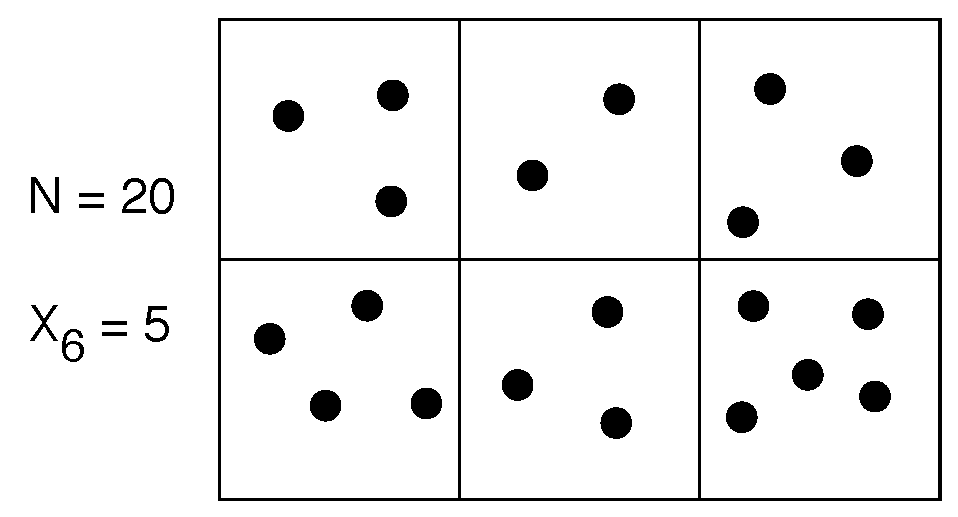
\includegraphics[width=0.5\textwidth]{figures/mlt/mlt-counting}
	\caption{MLT算法通过假设已知一个平均光照值${L}$,由于梅特波利斯算法的样本完全是服从目标函数分布的,所以我们可以通过数每个像素内样本值的数量来估计该像素的光照,如式\ref{e:mlt-counting}所示}
	\label{f:mlt-mlt-counting}
\end{figure}

有了上述的基本思路,剩下的问题是怎样计算平均光照值${L}$,而这正是我们要求解的结果。为了解决这个矛盾,\cite{a:MetropolisLightTransport}使用了从其他传统路径采样方法得到的光照贡献值来近似这个平均光照值,即:

\begin{equation}\label{e:mlt-unbiased}
	L_j\approx\hat{L}= \cfrac{L(X_0)}{p(X_0)} \cfrac{X}{N}
\end{equation}

这里$p$是任意一种传统的路径采样技术(例如双向路径追踪)得到样本$X_0$的概率。针对上式,我们需要回答的问题是,$p(x)$的选择会对该估计有着多大的影响,为此我们可以对上式进行方差分析。上式中两个分数部分可以看做是两个独立不相关的随机变量(注意这里第一个分数中的随机数$X_0$是随机选择的,所以整个分数$ \cfrac{L(X_0)}{p(X_0)}$仍然是一个随机数),假设两个分数部分分别表示为$A= \cfrac{L(X_0)}{p(X_0)}$和$B= \cfrac{X}{N}$,则可以得到:

\begin{equation}
	E(A)={L}\text{ , }
	E(B)= \cfrac{X}{{N}}
\end{equation}

$A$和$B$之所以可以看做不相关的是因为起始样本$X_0$的采样和后续梅特波利斯采样是两个独立的采样过程。由于$A$是单个随机变量,所以$V(A)$是一个由$p(X_0)$的形状决定的一个常数,同样$E(A)$是一个常数,而$V(B)$为$\Theta(1/N)$(\cite{a:AVarianceAnalysisoftheMetropolisLightTransportAlgorithm}),所以可以得到整个估计的方差为:

\begin{equation}
\begin{aligned}
	V(AB)&=V(A)V(B)+V(A)E(B)^{2}+V(B)E(A)^{2}\\
	     &=\Theta(1/N)
\end{aligned}
\end{equation}

由此可知,像素值估计$\hat{L}$的收敛并不受起始样本$X_0$的选择的影响。并且由于$E(A)={L}$,式\ref{e:mlt-unbiased}的估计是无偏的。

\begin{myshaded}
	读者可能会对这里的无偏性产生疑问,因为单个$X_0$的样本值几乎肯定会导致偏差,从而使整个估计是不正确的。但是这里不能把$A$项看做一个常数值,而应该是一个随机变量,尽管它只有一个值,但是该随机数变量的期望和真实值是相等的,因此是无偏的。但是这种有限的随机数数量会导致结果不正确,所以我们将在后面看到使用多个随机数来降低这种误差。
\end{myshaded}

尽管式\ref{e:mlt-unbiased}是无偏的,但是只使用单个起始样本则会导致不正确的结果(方差较大),例如${X}_0$路径完全可能被遮挡,从而导致$A=0$。为了使结果更准确,我们需要使用一个更大数量的(而不是一个)随机数${X}^{(1)},\cdots{X}^{(n)}$以更准确地计算平均光照值,例如\cite{b:pbrt}中使用了100000条初始路径来求整个图像空间的平均光照值。

通过这样的机制,MLT算法避免了起始偏差的问题。这样MLT算法大概可以分成两个阶段,即初始化阶段(initialization phase)\myindex{初始化阶段}{initialization phase},它对应于使用传统的双向路径采样以计算整个图像的平均光照值,以及梅特波利斯阶段(Metropolis phase)\myindex{梅特波利斯阶段}{Metropolis phase}。其中在梅特波利斯采样阶段,可以同时并行执行多个梅特波利斯采样线程,它们每个线程的起始路径可以从初始化阶段的所有样本中随机选择一个种子路径。在实践中,初始化阶段相对于梅特波利斯采样阶段的时间成本几乎是可以忽略不计的。

由此,完整的MLT估计可以写为:

\begin{equation}\label{e:mlt-estimate}
	m_j=E\Biggl[  \cfrac{1}{N}\sum^{N}_{i=1}W_iw_j({X}_i)\Biggl]
\end{equation}

上式中对于每个梅特波利斯样本的权重系数$W_j$都是相同的,即$W_j=W_0={L}={\rm \int} f$,它即是通过初始化阶段使用双向路径采样计算而来。因此上式相当于是对所有落于像素过滤器$w_j$内的样本进行计数。

\begin{myshaded}
	为什么这里的起始偏差可以被避免?这里理解的关键是,式\ref{e:mlt-mcmc}的估计是在极限情况下才成立的,即系统达到平稳分布,此时$p_i$收敛于$p$;而在趋近平稳分布的过程中,每个样本的贡献值其实还是需要通过$f_i/p_i$来计算,所以直接使用$f_i$代替就会呈现比较大的偏差,也即是式\ref{e:mlt-mcmc}早期的样本计算值是具有较大偏差的。而对于式\ref{e:mlt-estimate},由于其目标函数的期望值已经通过另一种采样方法估计出,所以它的每一个梅特波利斯样本计算的贡献值都是相对比较准确的,当然其准确度依赖于起始阶段对平均值的计算,但是相对于单个或少数样本值,平均值还是很容易获得比较精确的结果。
\end{myshaded}

这里讨论的避免起始偏差的估计方法其实仍然适用于其他对梅特波利斯采样方法的使用场景,但是这要求对应的目标函数可以使用一个不同于梅特波利斯算法的替代方法来获得目标函数的平均值,而这通常是比较困难的,例如目标函数没有归一化系数或者缺乏显式的反函数表示,因此传统的梅特波利斯蒙特卡洛方法仍然是使用式\ref{e:mlt-mcmc}表示的估计为主。

为此,MLT的算法可以总结为算法\ref{a:mlt-mlt}。

\begin{algorithm}
\begin{enumerate}
	\item 使用传统的双向路径追踪估计整个图像空间光照贡献的平均值$W_0={\rm \int}_{\mathcal{P}}f({\mathbf{x}}){\rm d}\mu({\mathbf{x}})$。
	\item 从上述用于计算平均光照贡献的样本中随机选择一个作为起始样本。
	\item 根据一定的样本数量$N$进行循环迭代,for $i$ = $1,\cdots,N$:
	\begin{enumerate}
		\item 根据建议转移函数$T({y}|{x}_i)$从${x}_i$产生一个建议样本。
		\item 根据接受概率$ \cfrac{f({y})T({x}_i|{y})}{f({x})T({y}_i|{x})}$接受或拒绝建议样本,如果接受则${x}_{i+1}={y}$,否则${x}_{i+1}={x}_i$。
		\item 将样本${x}_{i+1}$用于图像中的像素值计算。
	\end{enumerate}
\end{enumerate}
\caption{梅特波利斯光照传输基本算法描述}
\label{a:mlt-mlt}
\end{algorithm}

注意,上述的MLT算法是作用于一个标量的目标函数$f({x})$,而我们一般的光照贡献函数是RGB颜色矢量值,通常的方法是将颜色值转换为对应的亮度值,为了便于描述,上述(以及本书其他部分)的讨论并没有进行区分。

由此可以看出,上述过程中对于每个样本,3.c)步骤可以直接对多个包含该样本的像素进行计算,因为它仅仅是一个计数的计算,这又称为溅射法(splatting)\myindex{溅射法}{splatting},它将一个样本的贡献值直接溅射到周围覆盖的像素里去。然而在传统的方法中,每个像素的值来自于对多个路径积分的结果,因此每个路径通常仅用于单个像素值的计算。这是MLT算法不同于传统路径采样方法的一个方面,也因此大大提升了每个样本的利用率,提升了计算效率。梅特波利斯采样的样本可以在图像空间随机行走,算法结束后则每个像素都得到了计算,而不需要像传统双向路径追踪那样逐像素计算。当然这也有缺点,例如它不能使用第\ref{chp:path-tracing}章讨论的适应性采样。

针对上述的算法过程,MLT算法最重要的问题是选择合适的建议转移函数$T({y}|{x})$,它具体表现为针对当前路径执行一个突变操作以得到一条建议路径,通常涉及顶点的添加,移除以及移动等操作,跟重要性采样类似,可以通过设计不同的建议函数来探索一些特殊的目标路径。突变方法的选择几乎是本章将要讨论的不同MLT变种算法的核心内容,我们将在下一节介绍一些基本的突变策略,然后在后续的内容中介绍一些重要的改进方法。



\subsection{突变策略}\label{sec:mlt-mutations}
如第\ref{chp:mc}章的内容所述,梅特波利斯算法最主要的缺点,便是相邻的样本之间存在相关性,这种相关性增加了估计的方差,这些方差表现为,当建议转移的步幅过大时,更多的建议样本被拒绝,从而导致较低的接受率,随机数被卡在一些高频区域,形成噪点,如第\ref{chp:mc}章图\ref{f:mc-met-1}所示;而较低的转移步幅则又会导致非常慢的收敛速度。

\cite{a:MetropolisLightTransport}通过设计一组不同的路径突变方法来最大限度地减少估计的方差,这些突变策略通常都能满足一些不同的属性要求,并且它们可以按照类似重要性采样的原理进行组合。以下我们首先介绍为了减少误差,一个好的突变策略应该满足的属性要求,然后介绍原论文提出的几种突变方法,尽管现代更高级的方法都倾向于使用简单的单一突变方法来满足各种属性要求,但是学习这些基本的路径突变策略更有助于理解后面的内容。

\cite{a:MetropolisLightTransport}指出了好的突变策略应该具备以下属性:

\begin{itemize}
	\item \textbf{较高的接受概率 }如果所有样本的平均接受概率$a({y}|{x})$很低,则会导致路径样本序列中出现较多的重复路径${x},{x},\cdots,{x}$,这意味着同一路径在同一个像素点被计算多次,从而使这些点呈现为噪点。
	\item \textbf{较大突变能力 }即是对于大部分突变样本具有较大的接受率,由于样本之间的相关性,仍可能导致某些区域内的样本接受率极低(因此MLT算法通常不能使用一种固定的转移步幅),因此突变还需要具备较大突变的能力。
	\item \textbf{遍历性 }如果突变被限制在一定的范围,则随机行走的样本可能容易被卡在一些局部区域,所以突变需要具备遍历性(ergodicity)\mathindex{遍历性}{ergodicity}特征,即无论选择什么样的起始样本${X}_0$,随机行走的样本最终都能遍历系统的所有状态。很显然,在系统任意两个状态之间实现转移将有助于实现遍历性,即对于任意${x}$和${y}$,且$f({x})>0$和$f({y})>0$,都有$T({y}|{x})>0$。
	\item \textbf{图像空间的突变 }梅特波利斯样本之间是存在相关性的,但是我们不希望这种相关性会影响路径在图像空间的分布,即我们希望突变能够导致图像空间的位置变化,因为路径突变本身并不包含路径在图像空间分布的信息。
	\item \textbf{图像空间的均匀分布 }同上一条类似,除了希望路径样本能够在图像空间随机行走,我们还希望这些路径在图像空间的分布相对比较均匀,例如每个像素空间都能够接受足够数量的路径样本。
\end{itemize}

针对以上这些属性要求,\cite{a:MetropolisLightTransport}提出了三类突变策略(mutation strategies)\myindex{突变策略}{mutation strategies},即双向突变,微扰以及摄像机子路径突变(lens subpath mutation)\myindex{摄像机子路径突变}{lens subpath mutation}。这些突变策略各自都能够满足一定的属性要求,MLT算法能够将这些突变策略更有效地组合起来。




\subsubsection{双向突变}
双向突变(bidirectional mutation)\myindex{双向突变}{bidirectional mutation}是MLT算法最基础的突变策略,它能够通过修改路径长度,部分子路径等实现较大突变以及实现遍历性的能力。双向突变的基本思路是:对于当前路径${x}$,它首先按照一定的概率选择该路径的一段子路径,然后将该部分子路径替换为另一段随机产生(可能长度不一样)的子路径。

双向突变可以按以下步骤进行。首先,从当前路径${x}=\mathbf{x}_0\cdots\mathbf{x}_k$中选择一段需要删除(或被替换)的子路径$\mathbf{x}_s\cdots\mathbf{x}_t$,注意这里并不包含选择子路径的两个端点。路径中任意起始点被选择的概率表述为$p_d[s,t]$,它是两个操作概率的乘积,首先第一个因子$p_{d,1}$由当前路径的长度决定,它被设计为优先选择更短的子路径,这样的结果使得对当前路径的突变更小,因此更容易被接受,例如在\cite{a:MetropolisLightTransport}中,设$l_d=t-s$,他们选择的参数为$p_{d,1}[1]=0.25$,$p_{d,1}[2]=0.5$,对于$l_d\geq 3$,则使用$p_{d,1}[l_d]=2^{-l}$;第二个因子$p_{d,2}$用以避免较低的接受概率,我们将在本节后面再来讨论这个参数的选择。上述的过程将导致当前路径被分为两段:$\mathbf{x}_0\cdots\mathbf{x}_s$和$\mathbf{x}_t\cdots\mathbf{x}_k$。

接着,我们需要选择两个用于添加到顶点$\mathbf{x}_s$和$\mathbf{x}_t$末端的顶点的数量$s^{'}$和$t^{'}$,这也通过两个步骤来完成。首先选择要添加的子路径的总长度$l_a=s^{'}+t^{t}+1$的概率$p_{a,1}[l_a]$,为了保持较大的接受率,应尽可能使$l_a$的长度接近当前路径被删除的子路径的长度,因为这意味着对当前路径更小的突变,两条子路径更加相似,所以接受率更高。例如\cite{a:MetropolisLightTransport}使用的参数值为$p_{a,1}[l_d]=0.5$,$p_{a,1}[l_d-1]=p_{a,1}[l_d+1]=0.15$,剩下的概率则分配给其他允许的长度;然后需要选择特定的$s^{'}$和$t^{'}$的值,这通过对各种可能的组合分配相同的概率来设定$p_{a,2}$的值。

最后,分别从当前路径的两个片段的末端$\mathbf{x}_s$和$\mathbf{x}_t$分别使用传统路径追踪的增量的方式添加$s^{'}$和$t^{'}$个顶点,然后将两段子路径根据可见性关系连接起来形成新的建议路径。

从上述的过程可以看出,存在一定(虽然很小)的几率整个路径被一个全新的路径替换掉,这自动地满足了系统遍历性的要求。



\paragraph{接受概率}
对于上述产生新的建议路径${y}$的接受概率$a({y}|{x})$,根据式\ref{e:mlt-acceptance},其可表述为一个比值:

\begin{equation}
	a({y}|{x})= \cfrac{R({y}|{x})}{{x}|{y}}\text{ , } R({y}|{x})= \cfrac{f({y})}{T({y}|{x})}
\end{equation}

这里计算的关键是计算转移概率$T({y}|{x})$,根据前面的内容可以判断,它的值等于删除当前路径中的子路径$\mathbf{x}_s\cdots\mathbf{x}_t$的概率$p_d[s,t]$,以及添加$s^{'}+t^{'}$个新的顶点形成建议路径${y}$的概率的乘积。同样,根据这些参数的反向设定,可以求出$T({x}|{y})$的值。



\subsubsection{微~~扰}
上述的双向突变涉及对部分子路径的修改,这包括路径长度的变更等,这些操作的结果往往导致较大的突变,对于一些特殊的光照场景,双向突变的接受率会变得很低,例如一些包含焦散效果以及具有复杂可见性(例如仅通过很狭小的孔可见)等具有较大光照贡献的路径,此时较大的突变步幅使得样本很容易超出这些高贡献值区域,导致样本被拒绝。

针对这种场景,一种可行的方法便是减小突变的步幅,考虑到相邻的路径往往具有相似的光照贡献,所以接受率相对比较高,所以我们寻求一些能够搜索相邻路径的方法,这些方法由于具有较小的突变步幅,因此称为微扰(perturbation)\myindex{微扰}{perturbation}。

为了实现较小的扰动,\cite{a:MetropolisLightTransport}选择对摄像机端的部分子路径顶点进行轻微的移动,移动其他顶点也是可行的,但是这不能实现样本在图像空间的轻微移动。具体地,其包含两种轻微修改摄像机末端子路径的方法,透镜微扰和焦散微扰,如图\ref{f:mlt-mutations}所示。

\begin{figure}
\begin{fullwidth}
	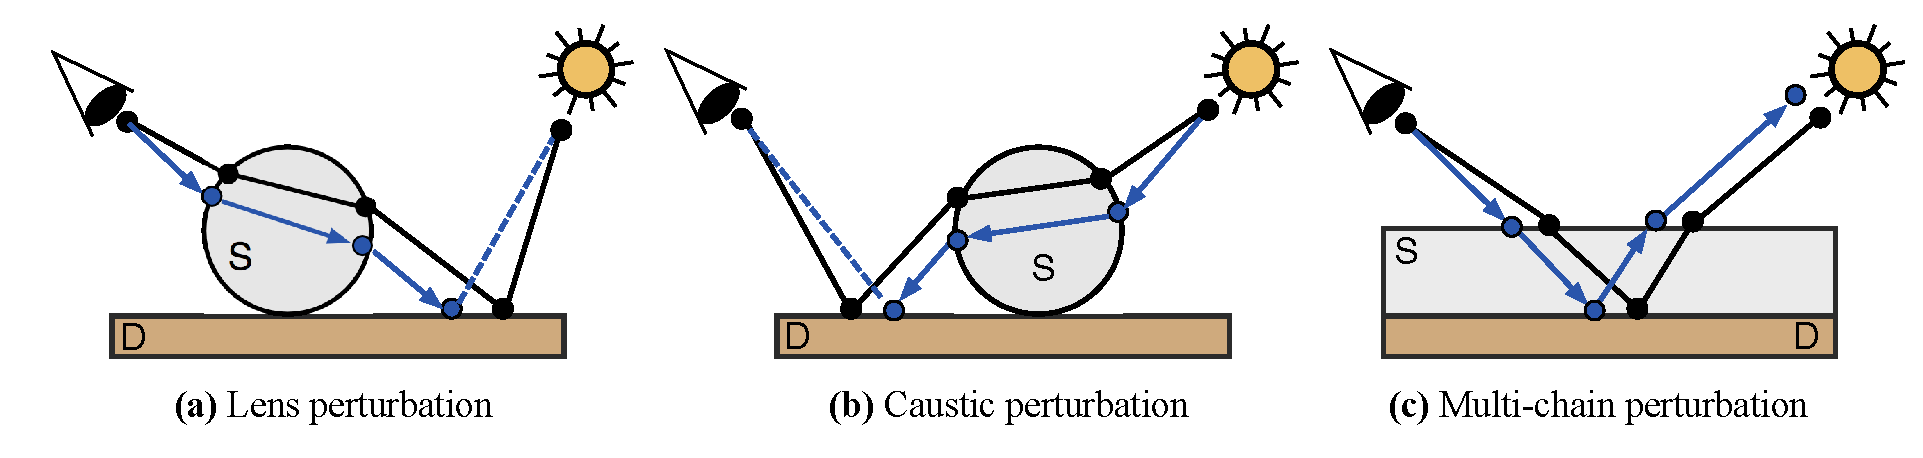
\includegraphics[width=1.0\thewidth]{figures/mlt/mutations}
	\caption{三种不同的微扰突变方法,这些方法尽可能地保持原路径的一部分不变,仅通过移动漫反射面上的顶点来实现对原路径轻微的突变,这样形成的两条路径具有相似的光照贡献,因此接受率增加}
	\label{f:mlt-mutations}
\end{fullwidth}
\end{figure}



\paragraph{透镜微扰}
对于一个形式为$(L|D)DS^{*}E$路径,其中摄像机末端的光泽/镜面路径$\mathbf{x}_t\cdots\mathbf{x}_k$称为透镜子路径(lens subpath),它从摄像机顶点出发直至达到第一个非光泽顶点,其路径长度为$k-t$,包含$k-t-1$个顶点。按相同长度替换一段透镜子路径的方法称为透镜微扰(lens perturbation)\myindex{透镜微扰}{lens perturbation},如图\ref{f:mlt-mutations}(a)所示。

为了替换一段透镜子路径,我们首先对当前路径在图像空间的位置沿一个随机的方向$\phi$移动一个随机的距离$R$,其中随机方向$\phi$沿图像空间均匀分布,而随机的距离$R$在两个输入参数$r_1<r_2$之间呈指数分布:

\begin{equation}
	R=r_2\exp(-\ln(\cfrac{r_2}{r_1})U)
\end{equation}

\noindent 其中,$U$为$[0,1]$上的均匀分布。在\cite{a:MetropolisLightTransport}中,参数$r_1=0.1$倍像素大小,而$r_2$的值使整个突变区域为整个图像区域的5\%大小。

为了替换一段相同长度的透镜子路径,我们对新产生的图像空间的建议顶点做增量式路径追踪,并让光线在场景中经过与删除的透镜子路径相同次数的反弹,然后连接该段新产生的透镜子路径与原路径的$x_{t-1}$顶点。如图\ref{f:mlt-mutations}(a)所示,由于光泽反射光线具有连贯性,所以产生的建议路径和原始路径具有一定的相似性,因此建议路径具有较高的接受率。




\paragraph{焦散微扰}
透镜微扰无法处理焦散路径,此时需要对透镜微扰相似的过程按相反的方向执行,即从光源开始替换一段光泽子路径,直到到达漫反射表面,然后直接与摄像机相连,如图\ref{f:mlt-mutations}(b)所示,这称为焦散微扰(caustic perturbation)\myindex{焦散微扰}{caustic perturbation}。



\paragraph{多链微扰}
对于路径中包含多段光泽顶点的路径,例如$(D|L)DS^{*}DS^{*}DE$,如图\ref{f:mlt-mutations}(c)所示,上述的两种微扰方法都是不够的,此时我们可以将多段光泽链执行微扰。这可以通过如图\ref{f:mlt-mutations}(c)所示的过程来实现,首先对透镜子路径执行一个透镜微扰,然后对于每个非光泽顶点,对对应的原始路径的方向做一个微扰以产生一个新的方向继续传播,这称为多链微扰(multi-chain perturbation)\myindex{多链微扰}{multi-chain perturbation}。




\subsubsection{透镜子路径突变}
为了使路径能够均匀分散于整个图像空间,并且提高建议路径的接受率,我们可以利用上述的透镜微扰(具有相同的部分路径,从而具有较高的接受率),但是让透镜子路径在全图像空间内突变来产生更均匀的样本分布。这称为透镜子路径突变(lens subpath mutation)\myindex{透镜子路径突变}{lens subpath mutation}。

为了实现透镜子路径在图像空间的均匀分布,\cite{a:MetropolisLightTransport}在内存中存储这一个当前透镜子路径,它通过随机从图像空间找到一个像素,然后选择一个方向开始光线追踪,直到到达第一个非光泽顶点,形成透镜子路径${x}_e$。当有路径的透镜子路径需要替换时,直接使用${x}_e$进行替换,${x}_e$可以被少量重复使用,然后又选择新的像素位置产生新的当前透镜子路径${x}_e$,其复用的次数远远小于种子路径的数量,以避免相同的透镜子路径被相同的路径使用多次。新透镜子路径产生的概率分布使得全图像空间的像素被均匀地覆盖到,最终使路径样本能够均匀分布于图像空间。




\subsubsection{总~~结}
上述这些突变方法都有自己的一些特征以及局限性,\cite{a:MetropolisLightTransport}进一步提出了一些方法使能够按照类似重要性采样的思路将这些突变方法组合起来,其组合的目标是使突变步幅尽可能地大,同时保持较高的接受率。

然而尽管如此,上述这些方法非常庞杂,缺乏统一的理论支持,并且这些方法严重依赖于一些与场景相关的参数设置,这里对其进行讨论的目的是了解路径突变的一些基本方法,例如对路径顶点,子路径及长度的修改。本章后面介绍的现代高级的MLT变种算法通常都是具有一些统一理论支撑的单一变种方法,这些突变方法具有更简洁的形式,实现起来也更加简单。




\section{原采样空间的突变策略}\label{sec:mlt-pssmlt}
上面介绍的路径空间(path space)\myindex{路径空间}{path space}并不是一个完整的欧几里得空间(Euclidean space)\mathindex{欧几里得空间}{Euclidean space},由于受场景复杂可见性的影响,路径空间往往只占据欧几里得空间的一个很小的子空间,这使得路径的采样变得复杂:它不能直接在欧几里得空间里对一个点进行任意采样,因为其包含的路径中的顶点可能根本不在任何物体表面上,也可能受可见性影响这条路径根本就是不存在的。

这意味着我们不能针对图像分布选择比较友好的全局性的重要性采样。

传统路径采样的过程是增量式的,它首先从光源(或摄像机)选择一个起始点,然后让光线在场景中传播,直到与摄像机(或者光源)相遇,在这个过程中每个步骤都会产生一个(或多个)随机数,例如选择随机像素上起点的位置,根据表面顶点BSDF属性随机选择反射或折射方向,以及根据俄罗斯轮盘选择终止概率等等。通常可以对其中单个步骤中随机数的选择使用重要性采样,例如针对BSDF的重要性采样以得到更接近于物体表面属性的方向分布,这种仅针对每一个步骤进行的重要性采样称为局部重要性采样(local importance sampling)\myindex{局部重要性采样}{local importance sampling},然而这种局部重要性远远不能反映全局的图像分布,因此路径样本产生较大的方差,例如如果光线的下一个方向使用针对光源的重要性采样,则采样得到的方向可能与顶点的BSDF分布不成正比;反之,如果我们根据BSDF分布选择下一个传播方向,则这些方向不能很好地适应光源的分布;尽管复合重要性采样通过组合多种采样技术进一步减少了平均方差,但是这离实际的图像分布仍然有较大的差距。

在上述路径采样的过程中,如果每一步都使用逆变换算法,则每一个步骤的单次采样都可以转换为对一个或多个[0,1]均匀分布采样,将整个路径采样过程中每个单个的采样过程组合起来,则构成一个高维的单位超立方体(unit hypercube)\myindex{单位超立方体}{unit hypercube},记为$\mathcal{U}\in[0,1]^{\infty}$,由于该空间提供了所有采样随机数的来源,我们称该超立方体构成的空间为原采样空间(primary sample space)\myindex{原采样空间}{primary sample space}。不同于路径空间,原采样空间是连续完整的,因此采样的过程变得更加直观和简单。

\cite{a:ASimpleandRobustMutationStrategyfortheMetropolisLightTransportAlgorithm}首先提出了在原采样空间对路径进行突变来实现MLT算法\footnote{原采样空间也被运用在传统的路径追踪技术中,通过对原采样空间采样产生更均匀分布的样本,来减少路径的方差,比如通过拟蒙特卡洛方法产生的一些高维高度均匀的样本等。},由于原采样空间的方法更简洁直观,且具有一些独特的优点,基于原采样空间的MLT方法已经成为现代MLT的一个重要分支和方向,本节将讨论这些基于原采样空间的MLT算法的原理,方法及其演变扩展。





\subsection{PSSMLT基本算法}\label{sec:mlt-pssmlt}
基于原采样空间的MLT算法称为原采样空间梅特波利斯光照传输(primary sample space Metropolis light transport,PSSMLT)\myindex{原采样空间梅特波利斯光照传输}{primary sample space Metropolis light transport},PSSMLT算法的主要思路是将原采样空间的一个点样本$\mathbf{u}$映射为路径空间的一条路径,然后在原采样空间执行梅特波利斯算法。

\begin{figure}
	\sidecaption
	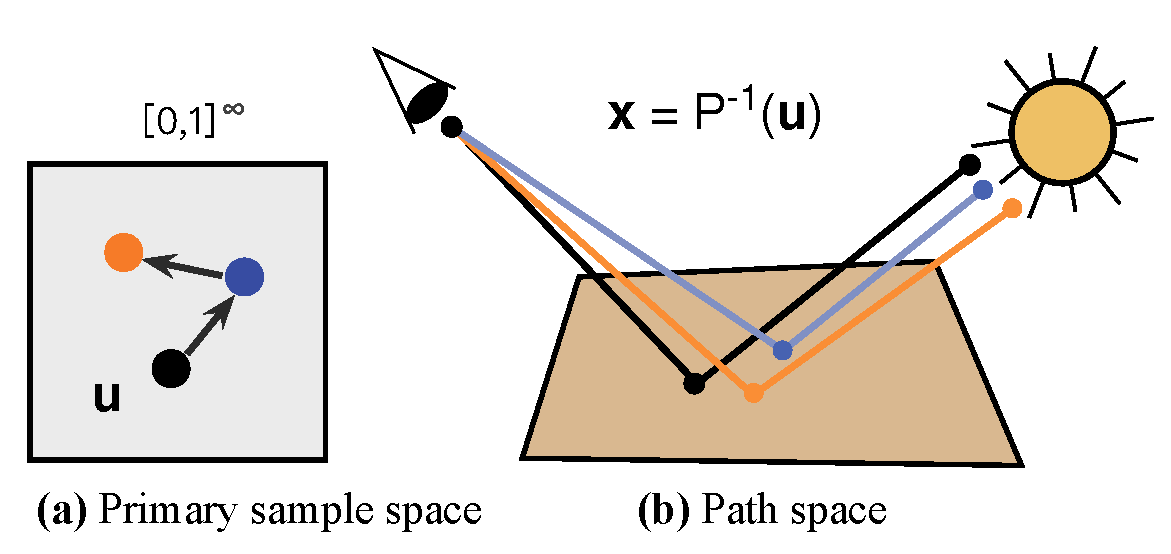
\includegraphics[width=0.65\textwidth]{figures/mlt/primary-space}
	\caption{原采样空间中的每个值表示路径空间中的一条路径,原采样空间可以看做是路径中随机变量的累积概率密度函数值所在的空间}
	\label{f:mlt-primary-space}
\end{figure}

设$\mathbf{z}$表示路径空间各个步骤(例如反射或折射对应的方向采样)对应的随机数构成的矢量\footnote{严格地说$\mathbf{z}$和一般的路径变量${x}$在数学上并不是相等的,例如${x}$中的一个顶点的BSDF方向采样需要两个[0,1]分布的随机变量,但它们表示的量的意义是相同的,因为它们之间具有确定的转换关系:路径采样根据$\mathbf{z}$的每个分量决定路径${x}$的构成,所以${x}$和$\mathbf{z}$可以看做是两个相同的量。},其概率密度为$p(\mathbf{z})$,根据原采样空间和路径空间的关系,如果设$P$表示路径空间样本$\mathbf{z}$的累积概率密度函数CDF,则原采样空间到路径空间的映射关系\footnote{注意,我们这里使用的是更易于理解的累积概率密度$\mathbf{u}=P(\mathbf{z})$的概念,它表示的是从路径空间样本$\mathbf{z}$到原采样空间样本$\mathbf{u}$的映射,其反函数就表示从原采样空间到路径空间的映射,这与\cite{a:ASimpleandRobustMutationStrategyfortheMetropolisLightTransportAlgorithm}中的关系是相反的,这更利于理解路径空间和原采样空间的关系。}可表示为:$\mathbf{z}=P^{-1}(\mathbf{u})$,如图\ref{f:mlt-primary-space}所示,因此我们可以得到原采样空间下的像素贡献积分为:

\begin{equation}\label{e:mlt-pssmlt-mapping}
\begin{aligned}
	{\rm \int}_{\mathcal{P}}f({\mathbf{x}}){\rm d}\mu({\mathbf{x}})&={\rm \int}_{\mathcal{U}}f(P^{-1}(\mathbf{u}))\bigg| \cfrac{{\rm d}P^{-1}(\mathbf{u})}{{\rm d}\mathbf{u}}\bigg|{\rm d}\mathbf{u}\\
	&={\rm \int}_{\mathcal{U}}f(P^{-1}(\mathbf{u})) \cfrac{1}{p(P^{-1}(\mathbf{u}))}{\rm d}\mathbf{u}
\end{aligned}
\end{equation}

\noindent 上式中,$\bigg| \cfrac{{\rm d}P^{-1}(\mathbf{u})}{{\rm d}\mathbf{u}}\bigg|$表示逆向映射的雅可比行列式,由于$P$表示$\mathbf{z}$的累积概率密度函数,如果$\mathbf{u}$是服从原采样空间的均匀分布,则该行列式的值的导数正好为路径空间样本$\mathbf{z}=P^{-1}(\mathbf{u})$的概率密度函数$p(P^{-1}(\mathbf{u}))$。

由此,我们得到原采样空间下的路径贡献值积分,其被积函数记为:

\begin{equation}
	\hat{C}(\mathbf{u})= \cfrac{\hat{f}(\mathbf{u})}{\hat{p}(\mathbf{u})}= \cfrac{f(P^{-1}(\mathbf{u}))}{\hat{p}(P^{-1}(\mathbf{u}))}
\end{equation}

\noindent 对应的标量贡献值为:

\begin{equation}
	\hat{C}^{*}= \cfrac{\hat{f}^{*}(\mathbf{u})}{\hat{p}(\mathbf{u})}= \cfrac{f^{*}(P^{-1}(\mathbf{u}))}{\hat{p}(P^{-1}(\mathbf{u}))}
\end{equation}

由于原采样空间$\mathcal{U}$中的样本$\mathbf{u}_1,\mathbf{u}_2,\cdots,\mathbf{u}_N$是[0,1]上的均匀分布,因此我们可以得到在原采样空间下像素的蒙特卡洛估计(参见式\ref{e:sum})为:

\begin{equation}\label{e:mlt-pssmlt-pixel}
	I_j\approx \cfrac{1}{N}\sum^{N}_{i=1} \cfrac{f_j(P^{-1}(\mathbf{u}_i))}{p(P^{-1}(\mathbf{u}_i))}
\end{equation}

毫无意外,这和路径空间下使用重要性采样的蒙特卡洛估计形式是一样的,其唯一的区别是原采样空间使用的是服从[0,1]的均匀采样,而路径空间的样本使用的是服从$p$的非均匀采样,由于原采样空间是路径空间概率密度$p$的累积密度函数所在的空间,所以两种不同空间下的估计才表现出一样的形式。因此将$\hat{C}(\mathbf{u})$代入传统的MLT算法中,便得到PSSMLT算法,如算法\ref{a:mlt-pssmlt}所示。

\begin{algorithm}
\begin{enumerate}
	\item 使用传统的双向路径追踪估计整个图像空间光照贡献的平均值$c^{-1}={\rm \int}_{\mathcal{U}}\hat{C}(\mathbf{u}){\rm d}\mathbf{u}$。
	\item 从上述用于计算平均光照贡献的样本中随机选择一个作为起始样本$\mathbf{u}_1$。
	\item 根据一定的样本数量$N$进行循环迭代,for $i$ = $1,\cdots,N$:
	\begin{enumerate}
		\item $\mathbf{v}=\begin{cases}
			\text{UniformRandom}()& \text{概率为:}p_{large}\\
			\text{Perturb}(\mathbf{u}_i)&\text{其他}
		\end{cases}$
		\item $\mathbf{u}_{i+1}=\begin{cases}
			\mathbf{v}& \text{概率为:} \cfrac{\hat{C}(\mathbf{v})}{\hat{C}(\mathbf{u}_i)}\\
			\mathbf{u}& \text{其他}
		\end{cases}$
		\item 将样本$\mathbf{u}_{i+1}$用于图像中的像素值计算。
	\end{enumerate}
\end{enumerate}
\caption{原采样空间梅特波利斯光照传输基本算法描述}
\label{a:mlt-pssmlt}
\end{algorithm}

相比传统的MLT算法,这里呈现几点差异:首先,如上所述,原采样空间使用的是[0,1]上的均匀采样,因此我们可以使用式\ref{e:mlt-pssmlt-pixel}来计算MLT算法需要的平均光照值$c^{-1}={\rm \int}_{\mathcal{U}}\hat{C}(\mathbf{u}){\rm d}\mathbf{u}$,这通过对$\mathcal{U}$均匀采样获取一个或多个样本实现,每个样本被使用(双向)路径追踪转化为一条路径,然后计算该路径的光照贡献值$f$及其概率密度$p$。
	
其次,由于原采样空间和路径空间是一一对应的,并且样本均匀分布,所以我们可以使用非常简单的建议转移函数,例如高斯分布,并且这些转移函数的计算不再需要复杂的与场景相关的一些参数;此外,这些建议转移函数通常是对称的,即$T(\mathbf{u}^{'}|\mathbf{u})=T(\mathbf{u}|\mathbf{u}^{'})$,所以在计算接受概率时,建议转移概率相关的项可以约掉,因此$a= \cfrac{\hat{C}(\mathbf{u}^{'}_i)}{\hat{C}(\mathbf{u}_i)}$。

最后,为了保证遍历性,PSSMLT使用了一个大步幅的突变,如上述算法中的1.a.中的UniformRandom(),它使用的样本完全独立于当前的马尔可夫链中的样本,如果一个大步幅的样本被接受,则它相当于产生了一个新的种子路径,开始一段新的马尔可夫链,这进一步减小了起始偏差。

为了减少样本间的相关性,大步幅突变的样本应该被最大限度地接受,因为在传统路径追踪技术中每一条合法的路径都是被接受的。当突变步幅较大时,建议转移的概率仅取决于目标状态,即:$T(\mathbf{u}_t|\mathbf{u}_t)=T(\mathbf{u}_t)$,再加上原采样空间的被积函数非常平滑,所以大部分突变的样本接受率可以表述为:

\begin{equation}
	a(\mathbf{u}_t|\mathbf{u}_t)= \cfrac{\hat{C}(\mathbf{u}_t)\cdot T(\mathbf{u}_i)}{\hat{C}(\mathbf{u}_i)\cdot T(\mathbf{u}_t)}\approx \cfrac{T(\mathbf{u}_i)}{T(\mathbf{u}_t)}
\end{equation}

由于大步幅突变样本$\mathbf{u}$是在原采样空间均匀采样得到的,因此各个样本的概率相同,因此上述的样本接受率接近于1,这很好地保证了状态空间的遍历性要求。我们还将在后面第\ref{sec:mlt-combine}节从平行回火的角度对大步幅突变给出一个更加严谨的解释。

除了上述这些算法层面的差异,使用原采样空间最大的好处来源于它可以减小估计的方差。这主要是因为我们对路径执行重要性采样,所以$f/p$会接近为一个常数,所以原采样空间的被积函数$\hat{C}$相对于路径空间的被积函数$f$更加平坦,因此具有更低的方差。同时,由于原采样空间的建议样本的接受率正比于建议样本和原样本贡献值的比值,即$a=\frac{\hat{C}(\mathbf{u}^{'}_i)}{\hat{C}(\mathbf{u}_i)}$,更平坦的$\hat{C}$分布导致更低的拒绝率。所以如果我们在原采样空间使用一个常数尺寸突变步幅,在原被积函数值$f$较大的区域,其步幅会被自动放大,而原被积函数值较小的区域,其步幅会被自动缩小,这避免了传统MLT算法中使用参数的方法根据路径特征适配各种突变方法的必要,使算法更简洁并且估计方差更低。

PSSMLT算法的第二个好处是,由于原采样空间和路径空间仅通过概率密度$p({x})$的累积密度函数$P$建立联系,因此原采样空间的样本$\mathbf{u}$与其对应路径空间的路径${x}$使用的具体采样技术是完全无关的,因此PSSMLT算法将路径采样看做一个黑盒子,例如我们可以使用(双向)路径追踪,光子映射或者其他任意路径采样技术,这简化了程序的结构。

然而,对路径采样的“一无所知”,也导致了PSSMLT算法的缺点,例如由于路径追踪通常使用如俄罗斯轮盘这样的技术来结束路径的深度,这导致路径长度并不是无限且通常不相等,因此它决定了使用的原采样空间的维度也是不同的,原采样空间通常没有足够的信息去预测路径空间样本的维度,例如原采样空间一个小的突变可能导致路径空间路径维度较大的变化,这称为涟漪效应;其次,在双向路径追踪中,一个原采样空间的样本更是可能产生多条长度不同,采样技术不同的路径,传统的双向路径追踪可以通过复合重要性采样等手段进行组合,但是PSSMLT算法缺乏很好的处理方式。

以下我们简单介绍原始PSSMLT算法对上述两个问题的解决方案和思路,我们还会在后面的改进算法中重新讨论这些问题的不同解决方式。




\subsubsection{最大值启发式}\label{sec:mlt-maximum-heuristic}
对于一个给定的原采样空间样本$\mathbf{u}$,如果我们仅使用单向路径追踪,则每个原采样空间样本被唯一映射到一条路径。例如假定以摄像机为起点,首先$\mathbf{u}_1$和$\mathbf{u}_2$被用来选择图像空间中的一个起点$\vec{x}_0$,然后沿摄像机到$\vec{x}_0$的方向做光线投射得到与场景的交点$\vec{x}_1$,针对$\vec{x}_1$,$\mathbf{u}_3$被用于决定是漫反射或光泽反射,然后$\mathbf{u}_4$和$\mathbf{u}_5$用于对BRDF分布采样得到新的路径的方向,以此类推直到路径与某个光源相交。

单向路径采样的效率极低,因此双向路径采样是更好的选择。然而当使用双向路径采样时,一个原采样空间样本$\mathbf{u}$将被影射到多条路径,每条路径都具有完全不同的概率,因为双向路径追踪可以分别给摄像机子路径和光源子路径分配不同的长度,并且所有这些子路径都可以相连形成长度不同的路径。

我们将在后面第\ref{sec:mlt-mmlt}节介绍一种扩展方法用于利用双向路径采样得到的多个路径,在这里为了保证每个原采样空间样本$\mathbf{u}$被映射为路径空间的一个唯一路径$\mathbf{z}$,它首先对所有通过可见性测试连接的长度不同的路径进行比较,选择贡献值最大的路径,然后针对该长度的路径,\cite{a:ASimpleandRobustMutationStrategyfortheMetropolisLightTransportAlgorithm}直接使用一种称为最大值启发式(maximum heuristic)\myindex{最大值启发式}{maximum heuristic}的方法,即只选择该路径所有不同采样技术中概率最大的路径作为$\mathbf{u}$的唯一映射路径。



\subsubsection{涟漪效应}
由于PSSMLT算法将路径采样技术视为一个黑盒子,并且原采样空间的维度肯定不能是无限的,因此一些原采样空间样本的突变可能引起路径空间路径较大的改变,这可能包括路径样本$\mathbf{z}$需要的随机数的数量超出原采样空间的维度,当路径的长度发生变化时,它代表了一种不同的采样技术,因此不能再使用之前较小维度的原采样空间。造成这些改变的原因称为涟漪效应(ripple effects)\myindex{涟漪效应}{ripple effects},在这里涟漪效应的意思是指,例如当路径中的某个路径发生较大的变化时,例如漫反射和光泽反射之间的选择,或者突变的光线超出了下一个表面的边界,这将引起后面一连串路径发生较大的变化,如图\ref{f:mlt-ripple-effects}所示。\cite{a:ASimpleandRobustMutationStrategyfortheMetropolisLightTransportAlgorithm}使用一种惰性计算(lazy evaluation)\myindex{惰性计算}{lazy evaluation}方法来动态地调整每个原采样样本的维度。

\begin{figure}
	\sidecaption
	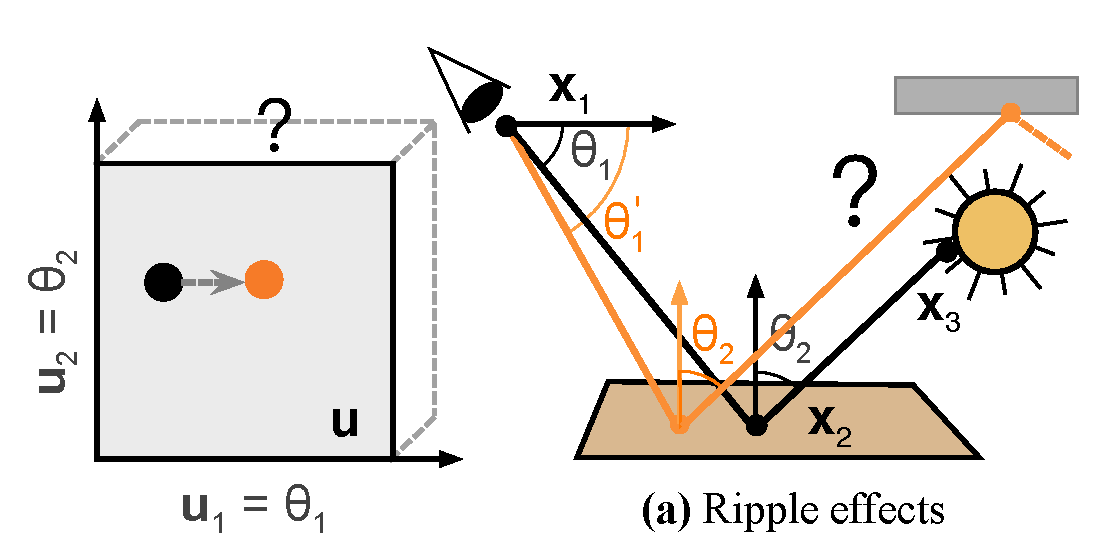
\includegraphics[width=0.65\textwidth]{figures/mlt/ripple-effects}
	\caption{对一个长度为2的路径执行突变,其中保持$\mathbf{u}_2$不变,将$\mathbf{u}_1$由$\theta_1$突变为$\theta^{'}_1$,在此几何配置中,由于第二条光线段超出了光源的尺寸范围,因此发生涟漪效应,整个路径的长度发生了变化,即是原采样空间的维度发生了变化,例如由2维变为3维甚至更多维}
	\label{f:mlt-ripple-effects}
\end{figure}

惰性计算的思路其实很简单,假设每个原采样空间的样本为$U\in[0,1]^{\infty}$,$U_i\in[0,1]$代表第$i$维度的随机数分量,假设$i$存在一个最大值$m$可以满足路径空间中最长路径的要求,则对于每一次原采样空间的突变,我们可以对当前的每一个分量$U_i$做一个微小的改变来获得新的突变样本。然而,由于涟漪效应,新的突变样本可能只使用$m$中的少数随机数分量,这里假设当前样本使用$n$个分量,那么$n$之后的$m-n$个分量的突变将是浪费的,如果以后还会出现长度大于$n$的路径,那么其中的一些突变还是有用的,但是如果后面由于不会出现长度大于$n$的路径,则这些维度随机数突变的计算都是浪费的。

\begin{figure}
	\sidecaption
	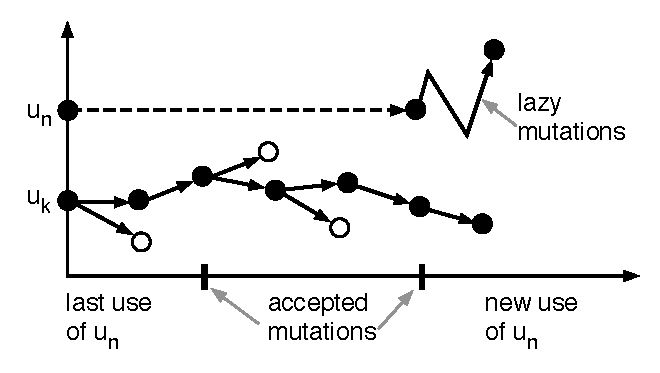
\includegraphics[width=0.65\textwidth]{figures/mlt/lazy}
	\caption{在惰性计算中,如果当前样本并不需要某个维度的随机变量,则不会对该维度的随机变量执行突变计算,直到后续的某个样本需要该维度的随机变量时再执行相应的计算;为了弥补延迟突变导致的该维度一连串突变的缺失,新的样本需要补回该维度错过的所有突变}
	\label{f:mlt-lazy}
\end{figure}

通过上面的分析可以看出,当当前路径需要使用第$i$个维度时,我们必须确保这个维度参与了自大步幅突变以来的每一次被接受的突变(因为大步幅突变以前的样本可以看做是跟当前马尔可夫链无关的,而被拒绝的突变不影响未来的样本),惰性计算就是将这个累积的突变计算延迟到了需要的时候:当当前样本不需要第$i$维度的随机数时(例如长度小于该维度),算法将不会对该维度的随机数执行突变计算;当当前样本需要对$X_i$执行突变时,则首先需要对该维度的随机数样本没有经历过(漏掉)的所有突变补充回来,如图\ref{f:mlt-lazy}所示。

算法\ref{a:mlt-lazy-evaluation}显示了一个基本的惰性计算算法,在该方法里,全局存储着一个不同维度的随机数的数组$u[]$,当产生一个新的样本$\mathbf{u}$时,它从1到$m$分别调用PrimarySample()函数得到每个维度的随机数样本$u[i].value$。PrimarySample全局存储着一个time变量用于记录从大步幅突变开始所有被接受的样本的数量,并且对于每个维度,随机数$u[i]$记录一个$modify$用来表示该维度随机数突变到了哪一步,每次新的样本使用第$i$维的随机变量$[u].i$时,算法要确保它之前的$time-modify$次累积突变需要被执行。

\begin{algorithm}
\begin{lstlisting}[language=C++, mathescape]
float PrimarySample(int i) { 
	if (u[i].modify < time) {
		if (large_step) {      // large step
			Push(i, u[i]);       // save state
			u[i].modify = time;
			u[i].value = random();
		} else {               // small step
			if (u[i].modify < large_step_time) {
				u[i].modify = large_step_time;
				u[i].value = random();
			}
			
			// lazy evaluation of mutations 
			while (u[i].modify < time-1) {
				u[i].value = Mutate(u[i].value);
				u[i].modify++;
			}
			
			Push(i, u[i]);      // save state
			u[i].value = Mutate(u[i].value);
			u[i].modify++;
		} 
	}
	return u[i].value;
}
\end{lstlisting}
\caption{获取每个原采样空间第$i$维的[0,1]随机变量的伪代码}
\label{a:mlt-lazy-evaluation}
\end{algorithm}

使用惰性计算的另一个好处是,其突变分布是一个标准的正态分布,例如:

\begin{equation}
	U^{'}_i\sim N(U_i,\sigma^{2})
\end{equation}

\noindent 这里$\sigma$是一个输入参数用于控制突变的步幅。

由于正态分布是一个指数形式的函数,因此多次突变的乘积可以合并为一个指数部分相加的形式,即$n$次突变可以合并为一次计算:

\begin{equation}
	U^{'}_i\sim N(U_i,n\sigma^{2})
\end{equation}

这大大了避免了许多重复的突变计算,使得最终算法几乎完全去掉了累积的计算过程。上述的算法被运用于\cite{b:pbrt}(第1033页)中。




\subsection{MMLT算法}\label{sec:mlt-mmlt}
传统的蒙特卡洛方法能够根据一个已知的概率密度分布$p$进行路径采样,然后计算该路径的光照贡献$f/p$,通过很好地设计不同的概率密度函数,例如根据BRDF分布,光源分布等进行重要性采样,蒙特卡洛方法能够很好地寻找具有不同特征的路径,例如双向路径追踪就擅长处理光源与主体场景不是直接可见的路径(如第\ref{sec:bidirectional-path-tracing}节所述)等。这些不同的概率密度函数对应一种不同的采样技术,同时结合复合重要性采样,传统的路径追踪技术更是能够处理各种不同几何配置的场景。

然而由于受限于$p$并不能完全近似未知的目标函数分布(例如双向路径采样受限于中间连接光源子路径和摄像机子路径时使用了直接连接两个末端点,而不是对其进行重要性采样),对于一些在$p$中概率很小然而$f$贡献值却很大的路径,传统的蒙特卡洛方法由于缺乏足够的样本,会导致收敛很慢,噪点很大。此时,另一种不依赖于构建一个假想概率密度的马尔可夫链蒙特卡洛方法则是一种更加有效的选择。

因为不依赖于任何概率密度分布,MLT算法中的样本是任意分布的,梅特波利斯采样算法根据样本之间的相关性来使样本集合服从目标函数的分布,这使得MLT算法能够处理如可见性比较复杂的场景,然而其收敛效率严重依赖于使用的样本突变技术,糟糕的突变技术将大大降低突变样本的接受率,而使得收敛速度非常缓慢。

为了减少路径样本的方差(从而提高接受率),PSSMLT提出了直接在路径的原采样空间进行突变,由于原采样空间的贡献值函数更为平坦,因此样本的接受率理论上可以得到较大的提升。然而PSSMLT算法虽然在原采样空间产生了比较好的突变样本,但这并不是直接的路径样本,而需要通过一个映射将原采样空间的样本转化为一条路径,由于它将路径采样看做一个黑盒子,因此原采样空间的样本可能被转化为一条较好或坏的路径样本,很不幸,在原始的PSSMLT算法中,这个转化过程并不是最优的,由于一条原采样空间的样本可以被双向路径采样转化为多条路径,而PSSMLT选择的依据是路径的最大概率(见第\ref{sec:mlt-maximum-heuristic}节的内容),而不是路径的最大贡献值,这就可能导致好的原采样空间样本被影射到比较糟糕的路径样本。

MLT算法和传统的蒙特卡洛方法(如路径追踪)都具有各自的优势与不足,因此我们设想能不能将两者结合起来,形成优势互补。这个想法看起来是不可行的,因为如上所述,传统的蒙特卡洛方法是根据一个已知概率密度采样的,而梅特波利斯算法是对任意分布进行采样的,尽管这个任意分布也可以是一般的路径采样方法,但是它们之间并没有直接的联系。直到PSSMLT的出现,它通过原采样空间和路径空间的一个映射来建立起了MLT算法和路径采样之间的联系。只是因为在使用双向路径采样时,原始的PSSMLT算法并没有考虑重要性采样选择最优的路径与原采样空间样本保持一一对应,\cite{a:MultiplexedMetropolisLightTransport}在此基础上对PSSMLT算法进行扩展使之能够考虑双向路径采样的重要性,这也是渲染领域第一次将复合重要性采样和MLT算法进行整合。




\subsubsection{模拟回火算法}\label{sec:mlt-simulated-tempering}
对于一个梅特波利斯状态空间,如果有一些额外的信息能够对这些状态空间进行划分,注意这里不是空间区域上的划分,而是某种重要性的划分,例如在不同参数控制下各个状态具有不同的接受率,则可以利用这些信息来提升梅特波利斯采样的效率。本节就首先介绍相关的理论,然后在下一节介绍怎样利用不同路径采样技术的重要性,来提升PSSMLT算法的效率。

在梅特波利斯算法\cite{a:EquationofStateCalculationsbyFastComputingMachines}的同一篇论文中,他们还提出了一种称为模拟退火(simulated annealing)\mathindex{模拟退火}{simulated annealing}的方法,该方法主要用于解决在梅特波利斯算法框架下的最优值(如最大值或最小值)问题。假设有一目标函数$q$,我们希望求其最小值,由于它有很多局部的最值,因此使用一般的局部比较方法并不能很容易找到全局的最值,此时我们需要使用梅特波利斯类似的采样方法,因为它有几率能够在全局空间内进行样本比较,从而能够有机会找到全局的最值,但可惜梅特波利斯算法主要用于解决采样问题,或者积分问题,而不是最优解问题,也就是说它对所有样本感兴趣,而不是对单个样本感兴趣。

在物理学中,退火是一种物理过程,金属物体在加热至一定的温度后,它的所有分子在状态空间自由运动,随着温度的下降,这些分子逐渐停留在不同的状态,在温度最低时,分子重新以一定的结构排列,达到能量最低的状态。

在物理退火冷却的过程中,实际上温度越高,分子之间状态的转移越活跃,我们可以认为分子越容易在全局各种状态之间转移;当温度下降时,分子活跃程度降低,分子将慢慢逐步限制在局部状态之间转移,最后趋于稳定。受此物理退火过程思路的启发,意识到马尔可夫链蒙特卡洛方法可以用来模拟系统状态在各种不同温度之间转移以达到热平衡,模拟退火算法可以通过以下方式来解决目标函数$q(x)$的最优值:

\begin{equation}
	h_{\uptau}(x)={\rm e}^{-q(x)/k\uptau}
\end{equation}

\noindent 这里$k$是一个任意的正常数,$\uptau$是一个控制参数。考虑对如上的概率分布$h_{\uptau}$执行梅特波利斯采样,当$\uptau$的值逐渐降低时,上述的概率分布在函数$q(x)$的全局最小值附近的概率最大,因此当$\uptau\to 0$时,上述的马尔可夫链的样本几乎完全分布在函数$q(x)$的全局最小值附近,这就是模拟退火的基本思想。

在上述模拟退火算法中,我们看到在不同温度下状态之间的转移具有不同的接受率,当然这不是说明状态的分布发生了变化,而是状态之间的转移变得更加“活跃”,而在梅特波利斯算法中,我们正希望寻找这种能够改善状态转移活跃度的方法,因为这可以加速梅特波利斯采样收敛的速度。

\cite{a:SimulatedTempering:ANewMonteCarloScheme}基于上述思路提出一种称为模拟回火(simulated tempering)\mathindex{模拟回火}{simulated tempering}的算法,模拟回火方法可以看做是模拟退火算法的一种反方法,它将一种能够影响状态转移活跃度的因子当做一个温度参数,然后对原始目标函数进行“加温”以寻找状态之间最快转移的路径,提升梅特波利斯算法采样的效率(即更快地遍历整个状态空间)。不过值得注意的是,模拟退火和模拟回火之间并无太多本质上的联系,尤其是模拟退火用于解决最优质问题(关注单个样本),而模拟回火解决梅特波利斯采样效率的问题(关注全部样本),这里介绍模拟退火的思路只是帮助建立对模拟回火算法比较直观的一些概念。

模拟回火包含两种相互可替代的方法:即平行回火(parallel tempering)\mathindex{即平行回火}{parallel tempering}和序列回火,平行回火\cite{a:markovchainmontecarlomaximumlikelihoodfordependentdata}相对容易使用,但是序列回火能解决更复杂的一些问题,并且效果更好。接下来我们将单独介绍序列回火,而把平行回火的讨论留到第\ref{sec:mlt-combine}节。




\paragraph{序列回火}
序列回火(serial tempering)\mathindex{序列回火}{serial tempering}
\cite{a:SimulatedTempering:ANewMonteCarloScheme,a:AnnealingMarkovChainMonteCarlowithApplicationstoAncestralInference,b:HandbookofMarkovChainMonteCarlo}在一个扩展的状态空间$(\mathbf{x},t)$上运行一个单一的马尔可夫链,这里$t$是一个$[1,m]$之间的正整数,$\mathbf{x}$表示目标函数的原始状态空间,我们的目标是要对一个和形式的分布$\sum^{M}_{t=1}f(\mathbf{x},T_t)$进行采样,$T_t$称为目标分布函数$f(\mathbf{x},T)$的参数。原始采样函数可以表示为:

\begin{equation}\label{e:mlt-serial-tempering}
	f(\mathbf{x})=\sum^{M}_{t=1}f(\mathbf{x},T_t)
\end{equation}

这里可以看做原始状态空间被参数$T$划分为多个序列空间。

为了遍历整个扩展状态空间$(\mathbf{x},t)$,除了要对每个特定参数$T_t$下的原始状态空间$\mathbf{x}$进行探索,还需要对各个参数空间$T$进行探索。序列回火算法的突变是一个组合的突变,其中一个基础的突变是在保持参数$T_t$不变的情况下,对状态$\mathbf{x}$执行突变,这和前面介绍的MLT方法是一致的,这又称为组件内更新\footnote{\cite{b:HandbookofMarkovChainMonteCarlo}中又称每个温度值为一个组件(component)。}(within-component updates)\myindex{组件内更新}{within-component update};另一个基础突变类型是在保持原始状态空间$\mathbf{x}$不变的情况下,对参数$T$进行突变,这又称为跳跃更新(jump updates)\myindex{跳跃更新}{jump updates}。与组件内更新类似,可以得到跳跃更新的接受率为$\min(1,r(T_t\to T_{t^{'}}))$,其中:

\begin{equation}
	r(T_t\to T_{t^{'}})=\frac{f^{*}(\mathbf{x},T_{t^{'}})q(T_{t^{'}}\to T_t)}{f^{*}(\mathbf{x},T_t)q(T_t\to T_{t^{'}})}
\end{equation}

\noindent 这里$q(T_{t^{'}}\to T_t)$表示从参数$T_t$向参数$T_{t^{'}}$转移的概率。通过引入跳跃更新,序列回火算法能够自动地访问那些使$f(\mathbf{x},T)$具有更大值的参数$T$的值,并且产生的样本服从式\ref{e:mlt-serial-tempering}的分布。

例如我们将在下面看到,通过指定不同的摄像机子路径和光源子路径的长度组合,双向路径采样将导致不同的采样技术,对于同一条路径,不同的采样技术具有不同的采样效率,因此路径的子路径长度的组合能够将原始状态空间划分成多个这样的序列,采样技术充当了这里的参数$T$,对于有些很难被采样的路径,也许通过改变使用的采样技术就能够更有效地进行采样。正是这样的思路,我们需要将序列回火技术引入到MLT算法中,以提高采样的效率。




\paragraph{原采样空间序列回火}
我们的目标是要将复合重要性采样引入到MLT算法中,即在不同的采样技术下(例如,在双向路径采样中,光源子路径和摄像机子路径长度的不同组合构成不同的采样技术),目标函数状态空间之间的转移具有不同的接受率,所以采样技术能够将目标函数原始状态空间划分成多个序列,然后我们可以利用上面介绍的序列回火技术来提升MLT算法采样的效率。

直观的想法是直接将序列回火技术引入的MLT算法中,然而实际上这是不可行的,因为MLT算法的突变样本是随机生成的(通过修改当前路径的顶点,长度等),它跟一个采样技术$p_i$无直接关联,或者说无法得知随着采样技术的变更,路径突变有着怎样效率的改变,因此无法在MLT算法中定义采样技术,以及采样技术对状态空间转移有着怎样的联系和影响;而在PSSMLT算法中,原采样空间样本到路径样本之间的映射是通过一种采样技术$p$的累积密度函数$P$的反函数建立的,具体地说,它将原采样空间的一个变量映射为使用某种采样技术得到的一条路径,因此采样技术在PSSMLT算法中能够影响原始状态之间的转移效率,即采样技术能够将原始状态空间划分为多个序列。\cite{a:MultiplexedMetropolisLightTransport}正是基于此提出了复合梅特波利斯光照传输,它将传统路径追踪中的复合重要性采样和MLT算法组合起来,具有更好的采样效率。

首先定义在原采样扩展空间下的目标函数形式。对于序列回火的目标函数,如式\ref{e:mlt-serial-tempering},温度函数$T$和原始目标函数是相互独立的,则式\ref{e:mlt-serial-tempering}可以改写为:

\begin{equation}\label{e:mlt-pssmlt-tempering}
	f^{*}({x})=\sum^{M}_{t=1}f^{*}_t({x})w_t({x})
\end{equation}

\noindent 这里$w_t$表示每种采样技术对应的权重系数,该系数在这里即表示序列回火中的温度函数,由复合重要性采样的内容可知,对于所有能够采样得到路径${x}$的采样技术,$\sum w_t=1$。

接着我们需要将原采样扩展空间的样本映射到路径空间,得到:

\begin{equation}
	\hat{f}^{*}({u})=\sum^{M}_{t=1}\hat{C}^{*}_t({u})\hat{w}_t({u})
\end{equation}

\noindent 这里$\hat{C}^{*}$的定义与PSSMLT算法一致,对于每个采样技术$t$对应的路径样本,它被使用路径的反向累积密度函数$P^{-1}_t({u})$进行转换;对于$\hat{w}_t({u})$,它和路径样本的映射方式一样,可以由路径空间的权重系数$w_t$的累计密度函数的反函数进行计算。需要注意的是,这里路径样本和权重系数的映射计算都是间接的,即不是通过显式的映射函数计算,而是首先根据原采样空间样本${u}$中的每个随机数使用增量的方式计算出一条路径,其中$\hat{w}_t$的值决定了路径的长度,进而计算出对应路径空间的权重值,我们将在后面进一步讨论路径贡献值的计算。

\begin{myshaded}
	权重系数实际是怎么映射的呢?
	
	当我们选定一个$t$值之后,实际上这唯一决定了路径中光源和摄像机子路径的长度,这样双向路径采样器按照这样的配置对路径进行采样并连接形成一条完整路径,然后我们将该路径所有可能的采样技术进行计算以得到当前采样技术的权重系数。
\end{myshaded}

有了上述这些理论基础,最终的采样过程可以将上述两个过程(即常规的原采样空间随机数的突变,以及采样技术的突变)联合起来,即给定扩展空间当前样本$({u},t)$和建议样本$({v},t^{'})$,我们可以得到建议样本的接受概率为$\min(1,a(({u},t)\to({v},t^{'})))$,其中:

\begin{equation}\label{e:mlt-mmlt-acceptance}
\begin{aligned}
	a(({u},t)\to({v},t^{'}))&=\frac{\hat{w}_{t^{'}}({v})\hat{C}^{*}_{t^{'}}({v})q(({v},t^{'})\to({u},t))}{\hat{w}_t({u})\hat{C}^{*}_t({u})q(({u},t)\to({v},t^{'}))}\\
	&=\frac{\hat{w}_{t^{'}}({v})\hat{C}^{*}_{t^{'}}({v})}{\hat{w}_t({u})\hat{C}^{*}_t({u})}
\end{aligned}
\end{equation}

\noindent 这里对于权重系数$t$的采样,我们将$m$种不同的采样技术映射到$[0,1]$区间,并且使用均匀采样,所以整个扩展空间样本的突变都是对称的,即:$q(({v},t^{'})\to({u},t))=q(({u},t)\to({v},t^{'}))$,所以上式的转移概率被约掉了。




\subsubsection{基本算法}
有了上述这些基础知识,以下我们便可以归纳出\cite{a:MultiplexedMetropolisLightTransport}提出的复合梅特波利斯光照传输(Multiplexed Metropolis Light Transport,MMLT)\myindex{复合梅特波利斯光照传输}{Multiplexed Metropolis Light Transport}算法,如算法\ref{a:mlt-mmmlt}和图\ref{f:mlt-mmlt}所示,它与PSSMLT算法的主体结构很相似,其主要的区别是包含一个额外的马尔可夫链状态用于决定一个原采样空间的样本怎样被映射为一条路径。

\begin{algorithm}
\begin{lstlisting}[language=C++, mathescape]
k $\leftarrow$ SAMPLEPATHLENGTH()
Proposal.$[{u}_k, u_{k,t}]$ $\leftarrow$ MUTATE(Current.$[{u}_k, u_{k,t}]$)
t $\leftarrow$ $\lfloor(k + 2)u_{k,t}\rfloor$
s $\leftarrow$ (k + 1) - t
EyePath $\leftarrow$ SAMPLEEYEPATH(Proposal.${u}_k, t$)
LightPath $\leftarrow$ SAMPLELIGHTPATH(Proposal.${u}_k, s$) 
Proposal.Contribution $\leftarrow$ COMBINE(EyePath, LightPath, $t, s$) 
a $\leftarrow$ Proposal.Contribution/Current.Contribution
if Random $\leq$ a then
	Current $\leftarrow$ Proposal
end if

ACCUMULATECONTRIBUTION(Current.Contribution)\end{lstlisting}
\caption{MMLT算法伪代码,它跟PSSMLT算法的结构相似,但是引入了路径长度的控制来更好地选择映射路径及计算贡献值}
\label{a:mlt-mmmlt}
\end{algorithm}

\begin{figure}
	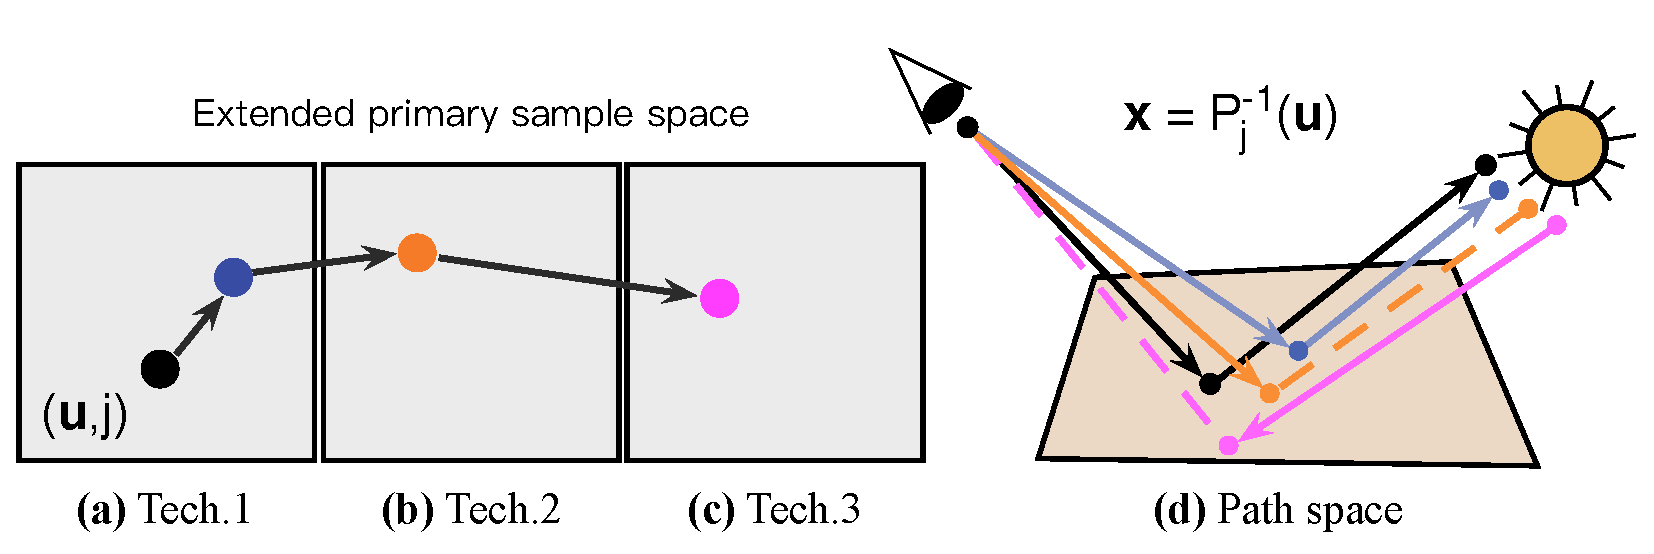
\includegraphics[width=1.0\textwidth]{figures/mlt/mmlt}
	\caption{MMLT算法通过增加一个路径长度控制参数,来使路径被限定为固定的长度,然后通过不同子路径的组合间接达到了选择不同采样技术的目的}
	\label{f:mlt-mmlt}
\end{figure}

在PSSMLT算法中,由于每个原采样空间的样本使用双向路径采样被映射到路径空间,对于给定路径长度,每个原采样空间的样本在路径空间包含多个对应的路径:首先双向路径追踪可以连接各个子路径的顶点形成多个长度不同的路径,其次,对于每个长度的路径,不同的采样技术对光照的贡献也是不一样的。对于前者,PSSMLT选择具有最大贡献值的长度的路径,对于后者,它是以最大值启发式选择概率密度最大的采样技术。这种映射显然是低效的,例如对于那些严重依赖于采样技术的路径,我们很难让梅特波利斯算法能够有效找到这样的路径,因此我们需要对采样技术的选择具有一定的控制能力。

与PSSMLT不同的是,尽管式\ref{e:mlt-pssmlt-tempering}可以包含在不同的路径长度之间进行突变,但是本质上不同长度的路径其对应的目标函数的维度是不同的,所以MMLT选择对每个路径长度使用一个单独的马尔可夫链,也即是说每个链内采样技术对应的路径长度是相同的,只是光源子路径和摄像机子路径的长度组合不同,以此形成不同的采样技术。

在算法\ref{a:mlt-mmmlt}中,由于引入了新的控制函数$\hat{w}_t$,对于一个给定长度为$k$的链,MMLT算法首先对$[0,1]$执行一个均匀采样,然后将得到的浮点结果映射到该路径对应的顶点数量$k+2$,并得到一个表示其中一个子路径顶点数量的整数值$t$;然后计算另一个子路径的长度$s=(k+1)-t$,它们分别被用于双向路径追踪中的摄像机子路径和光源子路径采样;最后我们按照式\ref{e:mlt-mmlt-acceptance}计算突变样本的接受率,与PSSMLT算法不同的是,由于这里指定了路径长度,所以MMLT只选择直接连接两条子路径的光线路径,同时对于该路径,MMLT会使用平衡启发式或更好的启发式来计算该路径的权重贡献值,而不是像PSSMLT一样使用最大值启发式。

MMLT算法\cite{m:MMLT}中原采样空间和路径空间样本值的突变如图\ref{f:mlt-mmlt}所示,相较于PSSMLT算法,它同时能够在原采样空间和路径长度之间进行突变,路径长度的选择间接导致了采样技术的选择,实际的采样技术其实还是由于算法\ref{a:mlt-mmmlt}中$t$和$s$两个参数决定的,但是对同一长度的多次突变,就能够有几率映射到各种不同的采样技术。通过这样的机制,当某些困难的路径严重依赖于采样技术时,在单个路径长度内的突变将使得接受率非常低,此时路径长度的突变将有利于提升突变的接受率,如图\ref{f:mlt-mmlt}(a)所示,而某些特定的采样技术就会有更高的概率被接受,从而找到这些非常困难的路径。






\section{路径空间的突变策略}\label{sec:pt-manifold}
原始的MLT算法完全依赖于随机的方式(即简单地随机替换当前路径的部分子路径)产生突变路径,这些突变策略往往不能有效地预测适当的步幅,从而导致非常低的接受率,使总的估计收敛速度非常缓慢;PSSMLT算法通过引入原采样空间,使MLT算法与传统的路径采样技术建立起了联系,由于传统的路径采样使用了(局部)重要性采样,因此对这种局部重要性进行控制的原采样空间突变策略能够有效地提升接受率,从而提升MLT算法的收敛速度。

然而,尽管具有上述的优点,由于基于原采样空间的MLT算法(如PSSMLT算法和MMLT算法)将路径采样技术看做一个黑盒子,因此原采样空间的突变策略仍不能有效地探索路径空间的局部重要性,例如由于涟漪效应,某个顶点在原采样空间的较小突变将可能产生一条变化非常大的路径;另一方面,对于MMLT算法,由于路径长度的突变形成了不同的采样技术,因此也可能形成较大的突变路径。这些不良的突变路径将导致非常低的接受率。

因此,为了更有效探索场景的局部特征,更好的基于路径空间的突变策略仍然是非常重要的。本节我们就介绍几种基于路径空间的突变策略,然后在第\ref{sec:mlt-combine-space}节会介绍怎样将原采样空间和路径空间的各种突变策略进行组合,以形成更高效的突变策略。




\subsection{流形探索}\label{sec:mlt-me}
包含有镜面或光泽表面路径的采样,一直是渲染领域一个比较棘手的问题,传统的路径采样方法都会使得光泽路径被采样的概率极低,而对于SDS路径,传统的采样方法更是几乎无法处理。同样,在MLT算法中,由于光泽路径不能被有效采样,使得带有较多光泽面的场景的渲染效率非常低。

为了提高光泽路径的采样效率,\cite{a:ManifoldExplorationAMarkovChainMonteCarloTechniqueforRenderingSceneswithDifficultSpecularTransport}提出了一种基于流形探索的采样方法,这种方法基于光泽路径的流形空间,通过分析一条当前光泽路径的局部几何特征(例如表面位置和法线的导数),以一阶泰勒近似得到一条突变路径,这种方法能够高效地得到一条准确的突变路径,因此能够有效地探索光泽路径,从而提高光泽路径的采样效率。

以下我们详细讨论这种方法的动机,原理,算法以及相关的一些知识。



\subsubsection{动机及流形}\label{sec:mlt-manifold}
传统的路径采样是基于从每个顶点处的方向采样,以增量的方式产生一条完整路径,例如如果每个顶点需要2个随机数用来对出射(或入射)方向进行采样,那么包含5个顶点的路径一共需要10个随机数,因此构成一个10维的路径空间$\mathcal{R}^{10}$(以下为了便于针对顶点而不是实际的空间维度进行讨论,我们将用符号$\mathcal{P}$来表示路径空间,例如一个10维的包含5个顶点的路径空间使用$\mathcal{P}_5$来表述,它等效于$\mathcal{R}^{10}$)。传统的路径空间是一个欧几里得空间(Euclidean space)\mathindex{欧几里得空间}{Euclidean space},即每条路径是$\mathcal{R}^{n}$中的一个点,然而由于受表面之间的可见性,镜面反射等的约束,所有路径构成的路径空间只是欧几里得空间的一个子空间。

这给路径的采样增加了难度,因为有许多路径都是无效的,例如双向路径采样中对于大多数镜面或光泽表面顶点之间的连接都是无效的,这也会大大降低MLT算法中突变路径的接受率。

在数学中,研究欧几里得空间子空间的分支称为流形上的微积分\cite{b:CalculusonManifolds:AModernApproachtoClassicalTheoremsofAdvancedCalculus,b:AnalysisOnManifolds},由于物理学中的很多拓扑结构都不是完整的欧几里得空间,所以针对欧几里得子空间的分析变得非常重要,然而由于一个任意拓扑空间可能具有非常复杂的数学表述,因此针对任意空间的分析会变得非常复杂,因此流形分析在任意空间拓扑和欧几里得空间建立起了联系,使之可以使用欧几里得空间的一些传统数学方法(如微积分)对任意的拓扑结构进行分析。

在数学中,流形(manifold)\mathindex{流形}{manifold}表示的是一个拓扑空间$\mathcal{S}$,该空间内每一个点邻近的某个局部空间可以近似为一个欧几里得空间。实践中,我们常对每个局部空间都可以映射为相同维度的流形感兴趣,称为$k$维流形,它表示的是$\mathcal{R}^{n}$的一个子空间,这里$0<k\leq n$,$k$维流形具有以下性质:即对于流形中的每一个点$\mathbf{p}\in\mathcal{S}$,存在一个包围点$\mathbf{p}$的开集$V$以及$\mathcal{R}^{k}$中的一个开集$U$,并且$V$和$U$之间存在一个唯一的连续映射$a:U\to V$。

图\ref{f:mlt-manifolds}展示了一个2维流形的概念,其中中间大图为$\mathcal{R}^{3}$内的任意一个流形,这个流形可能具有非常复杂的表述,但是其每个局部区域都可以唯一映射到$\mathcal{R}^{2}$的一个开集,如左上图和右下图所示。

\begin{figure}
\sidecaption
	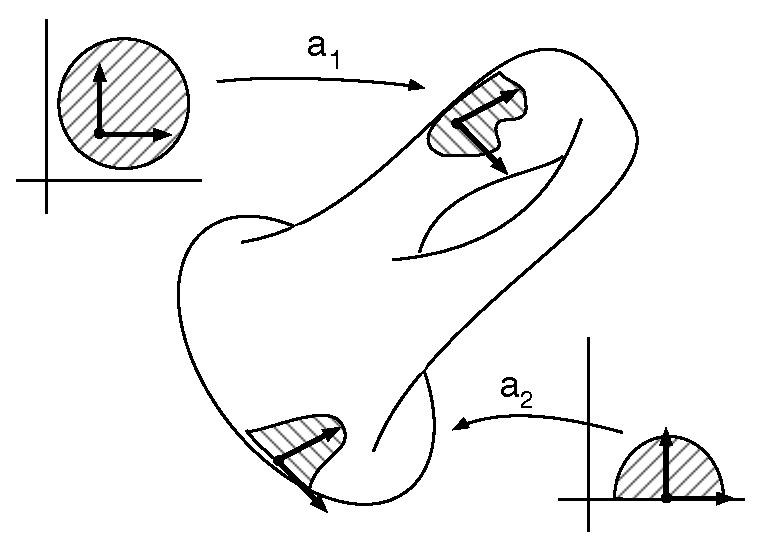
\includegraphics[width=.55\textwidth]{figures/mlt/manifolds}
	\caption{在数学中,流形表示的是欧几里得空间$\mathcal{R}^{n}$的一个子空间,并且流形的每个局部区域可以唯一映射为一个更低维度的欧几里得空间$\mathcal{R}^{k}$;图中中图表示一个3维欧几里得空间的一个流形,其每个局部区域可以映射为2维欧几里得空间的一个开集,因此该流形又称为2维流形}
	\label{f:mlt-manifolds}
\end{figure}

常见的1维流形如线段和圆形图形,2维流形为一个面,可以是平面或者球面等拓扑结构。比如对于单位圆形,其$\mathcal{R}^{2}$中的隐式函数可以表述为$x^{2}+y^{2}-1=0$,在该流形的全局范围内有$|y|=\sqrt{1-x^{2}}$,我们只能通过在$\mathcal{R}^{2}$空间内分析流形的性质,但是通过将圆形划分为$y\geq 0$和$y<0$两个局部区域,则我们可以通过一个1维的$x$值唯一确定一个$y$值,所以二维欧几里得空间的圆形变为一个一维流形。

通过将对复杂流形的分析转换为对局部欧几里得空间的分析,流形的分析变得非常简单,这样流形可以表述为一系列低维方程的组合,而不需要寻找复杂的全局方程,便可以以更低维度分析高维欧几里得子空间的问题。

流形的局部划分实际上表现为一个约束函数,它将某些维度限定在一定的范围,这些维度可以通过简单的分析或计算得出,从而实现了“降维”。例如通过限定$y\geq 0$或$y<0$,圆形的各个局部区域中$y$的值可以由一个$x$值唯一确定,因此这些局部区域可以看做是1维的。

实际上路径中也存在这种局部的约束,例如对于一条LDSDE路径,其中第三个顶点为镜面反射顶点,根据折射定理,镜面顶点处入射光线与法线的夹角等于出射光线与法线的夹角,并且两条光线与法线处于同一个平面,所以该路径可以表述为:

\begin{equation}
	(\overrightarrow {\mathbf{x}_x\mathbf{x}_2}+\overrightarrow{\mathbf{x}_3\mathbf{x}_4})||N(\mathbf{x}_3)
\end{equation}

\noindent 在上式中,$\overrightarrow {\mathbf{x}_x\mathbf{x}_2}+\overrightarrow{\mathbf{x}_3\mathbf{x}_4}$表示顶点$\mathbf{x}_3$处镜面反射的半矢量(half vector)\myindex{半矢量}{half vector},折射定理要求它必须平行于该点处的法线$N(\mathbf{x}_3)$,因此这对路径中的局部区域赋予了两个约束,使得顶点$\mathbf{x}_3$的位置最终可以由顶点$\mathbf{x}_2$和$\mathbf{x}_4$唯一确定。因此我们可以将该路径空间表述为$\mathcal{P}_5$上一个8维流形。

有了上述分析结果,我们更希望直接将路径积分表述为流形上的积分,而不是原始路径空间的积分。在接下来的内容中将看到,我们可以通过流形上局部参数化的方式,将整个路径表述为针对所有非镜面顶点的积分,即:

\begin{equation}\label{e:mlt-integral-on-manifold}
\begin{aligned}
	&\iiiint_{\mathcal{S}}f(\mathbf{x}_1\cdots\mathbf{x}_5){\rm d}\mathbf{x}_1{\rm d}\mathbf{x}_2{\rm d}\mathbf{x}_4{\rm d}\mathbf{x}_5\\
	=&\iiiint_{\mathcal{S}}L_e(\mathbf{x}_1\to\mathbf{x}_2)G(\mathbf{x}_1\leftrightarrow\mathbf{x}_2)f(\mathbf{x}_1\to\mathbf{x}_2\mathbf{x}_3)\underline{G(\mathbf{x}_2\leftrightarrow\mathbf{x}_3\leftrightarrow\mathbf{x}_4)R}\\
	&f(\mathbf{x}_3\to\mathbf{x}_4\to\mathbf{x}_5)G(\mathbf{x}_4\leftrightarrow\mathbf{x}_5)W_e(\mathbf{x}_4\to\mathbf{x}_5){\rm d}\mathbf{x}_1{\rm d}\mathbf{x}_2{\rm d}\mathbf{x}_4{\rm d}\mathbf{x}_5
\end{aligned}
\end{equation}

\noindent 在上式中,针对镜面顶点$\mathbf{x}_3$的积分消失了,贡献函数$f$仍然具有和原始路径空间的贡献函数相同的形式,即路径中每个顶点及边对应的相应项的乘积,但是对于每个镜面顶点一个具体的反射系数$R$代替了该点处对BRDF函数的计算,并且镜面反射处两个几何系数被合并为一个泛化几何系数$G(\mathbf{x}_2\leftrightarrow\mathbf{x}_3\leftrightarrow\mathbf{x}_4)$。

在光照公式由基于方向的积分向基于路径的积分形式的转换过程中,几何项$G$充当了变量替换的系数,即对于一个非镜面顶点,标准的几何项表示的是光线其中一个顶点的立体角,与该立体角投影到另一个顶点(面)处面积的比值,即是立体角相对于面积的导数,如图\ref{f:mlt-generalized-geometry-factor}(a)所示;泛化几何项(generalized geometry factor)\myindex{泛化几何项}{generalized geometry factor}可以通过类似的方式定义:即一条光泽路径其中一端顶点的立体角相对于另一端投影面积的导数,图\ref{f:mlt-generalized-geometry-factor}(b)显式了一个更复杂的例子。我们将在后面介绍怎样利用镜面流形的微分几何计算该泛化几何项。

\begin{figure}
	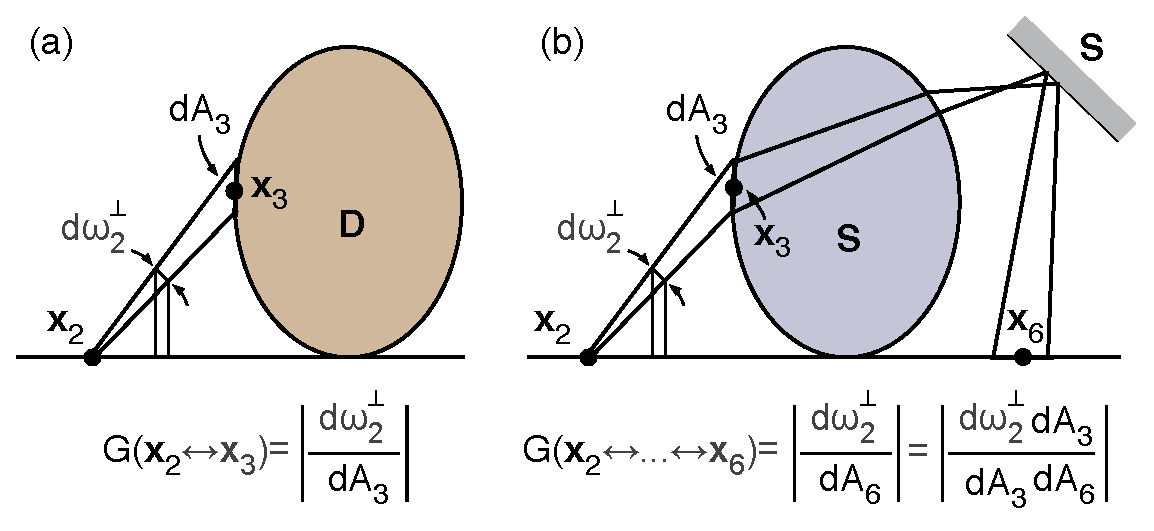
\includegraphics[width=\textwidth]{figures/mlt/generalized-geometry-factor}
	\caption{MMLT算法通过增加一个路径长度控制参数,来使路径被限定为固定的长度,然后通过不同子路径的组合间接达到了选择不同采样技术的目的}
	\label{f:mlt-generalized-geometry-factor}
\end{figure}

式\ref{e:mlt-integral-on-manifold}定义了光照公式基于镜面流形的积分形式,由于流形是通过局部约束定义的,接下来我们将介绍怎样定义镜面流形的局部约束,怎样求解泛化几何项,进而可以计算镜面流形的光照贡献。有了光线在镜面流形上的表述,我们将进一步介绍一种镜面流形上的突变方法,它可以直接有效地找出相邻的镜面路径,进而可以提高MLT算法中突变样本的接受率。




\subsubsection{隐函数定理}\label{sec:mlt-implicit-function-throrem}
为了理解路径流形探索相关的内容,我们有必要简单复习一下隐函数定理。

在数学中,隐函数(implicit function)\mathindex{隐函数}{implicit function}是指通过隐方程(implicit equation)\mathindex{隐方程}{implicit equation}定义的函数,隐方程是指形如$R(x_1,\cdots,x_n)=0$的方程,例如$x^{2}+y^{2}-1=0$就是单位圆的隐函数,隐函数通常没有直接的形式,而需要通过如隐函数定理等来求解其显式的形式。

流形通常就是通过隐函数进行定义的。设$f:\mathcal{R}^{n+m}\to \mathcal{R}^{m}$为一个连续可微的函数,将$f$写成$f(\mathbf{x},\mathbf{y})=f(x_1,\cdots,x_n,y_1,\cdots,y_m)$的形式,即$\mathbf{x}\in\mathcal{R}^{n}$,$\mathbf{y}\in\mathcal{R}^{m}$,我们的目标是求出一个显式的函数$g:\mathcal{R}^{n}\to\mathcal{R}^{m}$,使得$(\mathbf{x},g(\mathbf{x}))$正好是满足$f(\mathbf{x},\mathbf{y})=0$的所有$(\mathbf{x},\mathbf{y})$的集合。

如果$\mathbf{x}$和$\mathbf{y}$均是一个标量,则隐函数可记为$f(x,y)=0$,如果该函数决定了一个$y$关于$x$的函数$y=g(x)$,则根据导数的链规则,可得到隐函数关于$x$的导数方程为:

\begin{equation}
	\frac{{\rm \partial} f}{{\rm \partial} x}+(\frac{{\rm \partial} f}{{\rm \partial} y})g^{'}(x)=0
\end{equation}

\noindent 因此可以得到:

\begin{equation}\label{e:mlt-explicit-function}
	g^{'}(x)=-\frac{{\rm \partial} f/{\rm \partial} x}{{\rm \partial} f/{\rm \partial} y}
\end{equation}

即如果方程$f(x,y)$在某个点$(a,b)$处具有${\rm \partial} f/{\rm \partial} y\neq 0$,那么对于$a$点附近的$x$,$g$决定了$y$关于$x$的一个函数,并且这个函数是可微的。

通常$\mathbf{x}$和$\mathbf{y}$都是多元变量,因此上式中的导数需要替换为雅可比矩阵(Jacobian matrix)\mathindex{雅可比矩阵}{Jacobian matrix},表示分别对每个分量的偏导数的矩阵,我们用$Df$来表示,则$(\mathbf{a},\mathbf{b})$处的雅可比矩阵可表示为:

\begin{equation}\label{e:mlt-jacobian}
	(Df)(\mathbf{a},\mathbf{b})=\begin{bmatrix}[ccc|ccc]
		\frac{{\rm \partial} f_1}{{\rm \partial} x_1}(\mathbf{a},\mathbf{b})&\cdots &\frac{{\rm \partial} f_1}{{\rm \partial} x_n}(\mathbf{a},\mathbf{b}) &\frac{{\rm \partial} f_1}{{\rm \partial} y_1}(\mathbf{a},\mathbf{b})&\cdots &\frac{{\rm \partial} f_1}{{\rm \partial} y_m}(\mathbf{a},\mathbf{b})\\
		\vdots & \ddots & \vdots & \vdots & \ddots & \vdots \\
		\frac{{\rm \partial} f_m}{{\rm \partial} x_1}(\mathbf{a},\mathbf{b})&\cdots & \frac{{\rm \partial} f_m}{{\rm \partial} x_n}(\mathbf{a},\mathbf{b}) &\frac{{\rm \partial} f_m}{{\rm \partial} y_1}(\mathbf{a},\mathbf{b})&\cdots & \frac{{\rm \partial} f_m}{{\rm \partial} y_m}(\mathbf{a},\mathbf{b})
	\end{bmatrix}=[\mathbf{X}|\mathbf{Y}]
\end{equation}

\noindent 其中,$f$是由$m$个方程组成的包含$n+m$个未知量的标量方程组,我们希望能够任意指派$n$个未知量(即$\mathbf{x}$)的值并用这些未知量解出其他$m$个未知量(即$\mathbf{y}$)的值。这里隐式方程组对$\mathbf{x}$和$\mathbf{y}$的雅可比矩阵分别记为$\mathbf{X}$和$\mathbf{Y}$。

有了上述基础知识,隐函数定理(implicit function theorem)\mathindex{隐函数定理}{implicit function theorem}指出,如果对于$(\mathbf{a},\mathbf{b})$使得$f(\mathbf{a},\mathbf{b})=0$,且:

\begin{equation}
	det\frac{{\rm \partial} y}{{\rm \partial} \mathbf{y}}(\mathbf{a},\mathbf{b})\neq 0
\end{equation}

\noindent 那么在$\mathcal{R}^{n}$上存在$\mathbf{a}$的一个邻域和唯一的一个连续函数$g:\mathbf{R}^{n}\to\mathcal{R}^{m}$使得$g(\mathbf{a})=\mathbf{b}$,且对于所有该邻域的$\mathbf{x}$有$f(\mathbf{a},\mathbf{b})=0$。

通过式\ref{e:mlt-jacobian}可以很容易得知所有$\mathbf{y}$关于$\mathbf{x}$的方程为:

\begin{equation}\label{e:mlt-explicit-g}
	Dg(\mathbf{x})=-\biggl[\frac{{\rm \partial} f}{{\rm \partial}\mathbf{y}}(\mathbf{x},g(\mathbf{x})) \biggl]^{-1}\cdot\frac{{\rm \partial} f}{{\rm \partial}\mathbf{x}}(\mathbf{x},g(\mathbf{x}))=-\mathbf{Y}^{-1}\cdot\mathbf{X}
\end{equation}

\noindent 其中,$\cfrac{{\rm \partial} f}{{\rm \partial}\mathbf{y}}$是一个$m\times m$矩阵,它表示隐式方程组对所有待计算未知量$\mathbf{y}$的雅可比矩阵。

根据隐式函数定理,我们可以求出一个隐式方程组中变量$\mathbf{y}$的导数形式,如果我们能够将一条路径表述为流形上的积分形式,便可以根据一阶泰勒近似求出一条该路径附近的突变路径,这样的路径由于是根据流形而不是路径空间得出的,因此通常是一条更精确的光泽路径。





\subsubsection{镜面流形几何}
在本章前面介绍的突变策略中,不管是基于路径顶点的修改(如原始MLT算法),还是基于原采样空间的突变(如PSSMLT或MMLT算法),这些本质上都可以归结为对路径出射方向的突变,由于出射方向永远不了解场景的特征,因此它们很难产生有效的突变路径;而通过第\ref{sec:mlt-manifold}节的分析,反射和折射定理对路径的局部形成了一个约束,它要求反射或折射形成的半矢量必须和法线重合,这种联系使我们有机会去挖掘路径在场景中的局部特征,从而能够更有效的找到突变路径。

本节和后面第\ref{sec:mlt-hslt}节都是尝试将路径空间的路径表述转换为某种由物体局部空间构成的一种流形上,例如本节的镜面流形以及第\ref{sec:mlt-hslt}节的半矢量空间,将路径转换到这些局部流形上,使得我们可以利用物体表面的位置和法线的导数等几何信息探索更有效的突变路径。与前面的方法相比,这些突变路径的接受率更高,因为它们反应了物体表面的局部特征。

首先我们来归纳一下这两种突变策略的基本思路,以便于能够带着这些思路更好理解下面的内容,初学者在理解流形探索相关内容的时候会感到非常吃力,它不但涉及比较复杂的数学知识,也包含比较抽象的算法描述,所以带着基本思路能够更好更容易地理解后面的内容。

我们将这些流形探索的思路归纳如下:

\begin{itemize}
	\item 首先,使用传统采样方法(例如双向路径采样)得到一条路径,该路径作为当前路径,后面将使用流形探索的方法对当前路径进行突变。
	\item 其次,为了在流形上对当前路径进行突变,我们需要将当前路径的表述转换到流形上,这包括计算不同空间之间变量替换的雅可比矩阵;同时根据隐函数定理,我们能够写出某些待突变的顶点关于其他一些(固定不动的)顶点的函数(导数)。
	\item 最后,当我们得到各个突变顶点关于不动顶点的导数之后,则我们能够使用一阶泰勒近似得到当前路径的一条突变路径,这些包含局部信息的导数使得突变路径具有较高的接受率。当然在实际上直接使用泰勒近似会使得某些突变顶点可能不在表面上,这里会使用牛顿迭代法的一种变体来保证得到合法的突变路径。
\end{itemize}

\begin{myshaded}
	注意,由于事先并不知道场景的局部几何信息,我们并不能直接从镜面流形上对路径进行采样,它必须依赖于一条已知路径,因为已知路径提供了场景的局部信息,如位置和法线导数等,进而可以使用一阶泰勒近似计算该路径附近的一条突变路径。因此流形探索不能用于传统蒙特卡洛方法的直接路径采用,只能用于马尔可夫链蒙特卡洛方法中。
\end{myshaded}

通过上面的分析,流形探索的思路其实就非常清晰了,它其实就是对于一个函数$f(x)$,并已知一个点$x_0$的值$f(x_0)$(这里对应当前路径)以及该函数在$x_0$处的导数$f^{'}(x_0)$,然后利用一阶泰勒近似计算$x_0$附近一个点的值$f(x)=f(x_0)+f^{'}(x_0)\Delta x$。

当然在这里函数变量不是一个标量,而是一个路径矢量${\mathbf{x}}$,因此导数变为雅可比矩阵;其次,从传统的路径形式的被积函数中,我们无法得知其关于每个顶点处的导数,因此我们无法在路径空间进行泰勒近似计算;而反射和折射定理给了我们一种光线的局部约束,这种约束能够提供局部的几何信息,因此我们需要将路径空间的被积函数转换到镜面流形上,然后执行上述一阶泰勒近似计算;最后得出的近似值即是一条突变路径。

有了上述这些概念,本节我们将首先介绍镜面流形几何相关的知识,例如怎样将当前路径表述在镜面流形上,怎样解空间变换导致的雅可比矩阵,以及求解各个待突变顶点相对于其他顶点的函数。




\paragraph{路径在镜面流形中的表述}
首先,我们需要将一个当前路径${\mathbf{x}}$的表述变换到镜面流形空间上。

当前路径提供了各个顶点的几何信息,例如顶点的位置,法线以及位置和法线的导数,而反射和折射定理提供了各个顶点与其相邻顶点之间的一种联系,即一个约束函数,所有镜面顶点的约束函数就构成了一个镜面流形上的表述。

为了便于表述,我们将路径中所有的顶点都划分为光泽顶点或漫反射顶点,因此一个长度为$k$的路径可以表述为$\{D,S\}^{k}$,特别地,点光源或平行光源定义为$D$,而摄像机或面积光源上的顶点定义为$S$。有了上述的路径表述,对于每一个镜面顶点$S$,我们可以对其赋予一个约束函数(constraint function)\mathindex{约束函数}{constraint function},该约束函数涉及该顶点与其相邻的两个顶点;

\begin{equation}\label{e:mlt-constraint-function}
	\mathbf{c}_i(\mathbf{x}_{i-1},\mathbf{x}_i,\mathbf{x}_{i+1})=\mathbf{0}
\end{equation}

上述的约束函数表示什么量或者说具有什么意义呢?对于镜面顶点$\mathbf{x}_i$,上述的约束函数根据相邻两个顶点的方向计算满足反射或折射定理的半矢量$h$,并将该半矢量投影在顶点$\mathbf{x}_i$的正切空间内形成两个矢量。绝对的镜面反射要求该半矢量与$\mathbf{x}_i$处的法线重合,因此两个正切空间的投影矢量将为$0$。通过这种约束,镜面顶点$\mathbf{x}_i$可以看做其相邻顶点$\mathbf{x}_{i-1}$和$\mathbf{x}_{i+1}$的函数。

根据\cite{a:Microfacetmodelsforrefractionthroughroughsurfaces},镜面反射和折射都可以计算出一个统一的泛化半矢量,因此镜面反射和折射可以表述为一个统一的约束函数:

\begin{equation}\label{e:mlt-constraint-function-and-half-vector}
\begin{aligned}
	\mathbf{c}_i(\mathbf{x}_{i-1},\mathbf{x}_i,\mathbf{x}_{i+1})&=T(\mathbf{x}_i)^{T}h(\mathbf{x}_i,\overrightarrow{\mathbf{x}_i\mathbf{x}_{i-1}},\overrightarrow{\mathbf{x}_i\mathbf{x}_{i+1}})\\
	h(\mathbf{x},\mathbf{v},\mathbf{w})&=\frac{\eta(\mathbf{x},\mathbf{v})\mathbf{v}+\eta(\mathbf{x},\mathbf{w})\mathbf{w}}{||\eta(\mathbf{x},\mathbf{v})\mathbf{v}+\eta(\mathbf{x},\mathbf{w})\mathbf{w}||}
\end{aligned}
\end{equation}

\noindent 这里$T(\mathbf{x})$是一个矩阵,它的两个列形成顶点$\mathbf{x}$处的正切空间(平面)的两个基坐标。$\eta(\mathbf{x},\mathbf{v})$表示光线$(\mathbf{x},\mathbf{v})$对应的折射率。

特别地,路径中的镜面端点仍然能够引入约束,例如对于路径起点为平行光源或顶点光线的情况,该子路径的方向$\mathbf{x}_1\to\mathbf{x}_2$是固定的,这引入一种特殊的约束函数:

\begin{equation}
	\mathbf{c}_1(\mathbf{x}_1,\mathbf{x}_2)=T(\mathbf{x}_1)\overrightarrow{\mathbf{x}_1\mathbf{x}_2}
\end{equation}

通过式\ref{e:mlt-constraint-function},我们隐式地在一个局部参数化正切空间$\mathcal{R}^{2}$定义了点$\mathbf{x}_i$,这种定义仅对于$\mathbf{x}_i$附近的局部区域是合法的,它不适用于其他顶点的局部区域,注意这里每个顶点需要一个二维顶点$\mathcal{R}^{2}$来表示,因为它仅在该点所在的正切空间被表述。这种局部参数化的正切空间的定义可以是任意的,从后面可知,我们需要的仅仅是每个顶点的位置导数和法线导数。这些导数可以从顶点所在的曲面的参数化表述中(如一般的参数曲面或者三角形网格等)获得,如后面的内容所述。

因此,对于一个长度为$n$,其中包含$p$个镜面顶点的路径,我们可以将所有这些镜面顶点的约束函数组合起来,形成一个约束方程组$C:\mathcal{R}^{2n}\to\mathcal{R}^{2p}$,这个约束方程组形成一个镜面流形(specular manifold)\mathindex{镜面流形}{specular manifold}:

\begin{equation}\label{e:mlt-manifold}
	\mathcal{S}=\{{\mathbf{x}}\mid C({\mathbf{x}})=\mathbf{0}\}
\end{equation}

上述的约束方程组的形式如图\ref{f:mlt-manifold-constraint}(b)所示,它实际上是一个总共包含$n$个未知变量,以及$p$个约束函数构成的方程组。将路径转换到镜面流形上使得我们可以很方便地探索一个特定路径的局部邻域,前面介绍的隐函数定理保证了在局部空间内存在一种显式函数关系$q:\mathcal{R}^{2(n-p)}\to\mathcal{R}^{2p}$,该函数说明所有镜面顶点是关于所有非镜面顶点的函数,而函数$q$的导数$q^{'}$(这里是一个雅可比矩阵),则正是流形上某个顶点的局部正切空间,这可以很容易地从约束方程组$C$计算得出。进一步,有了这种局部坐标下的导数,我们可以使用一阶泰勒近似来得到当前路径附近邻域内的一条路径。

\begin{figure}
\begin{fullwidth}
	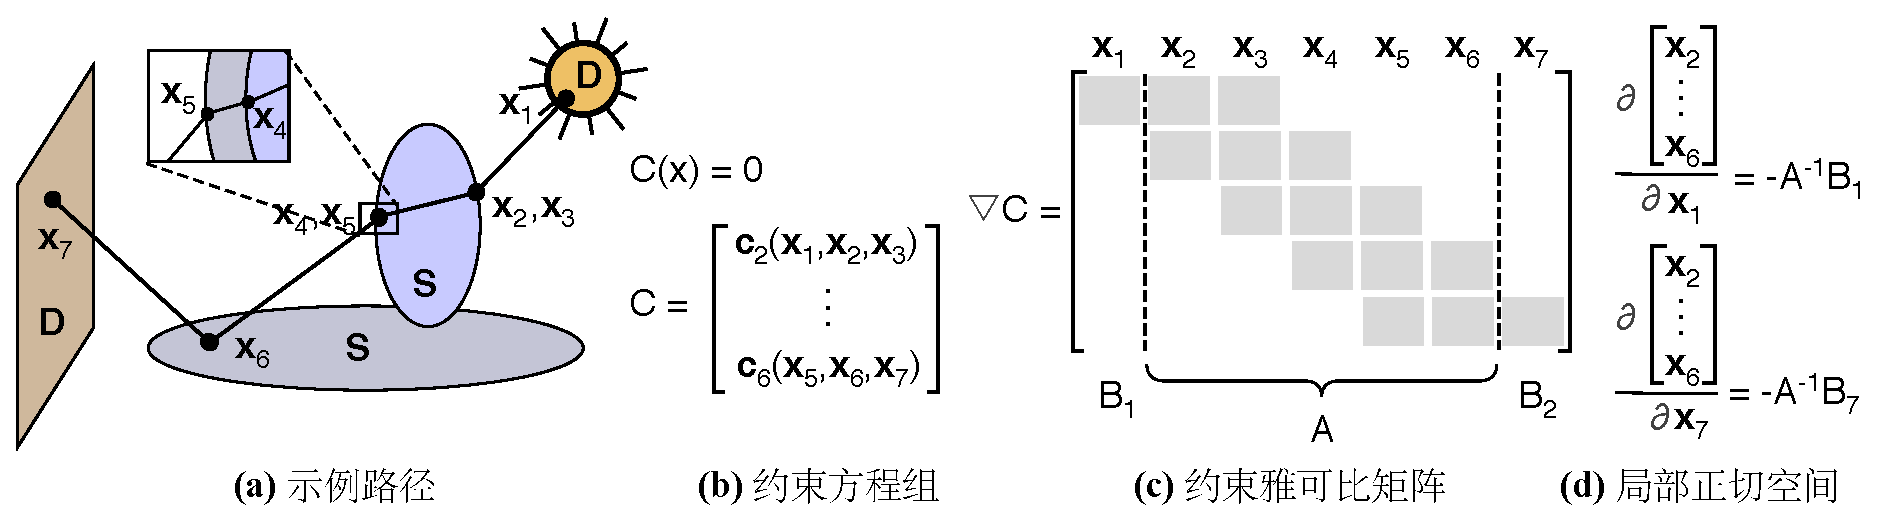
\includegraphics[width=1.0\thewidth]{figures/mlt/manifold-constraint}
	\caption{(a)展示了一条两端为漫反射顶点,中间其他顶点为镜面顶点的路径;这条路径通过各个镜面顶点处的约束方程组(b)被转化到镜面流形上;(c)为该约束方程组导数;最后根据隐函数定理,可以求出各个镜面顶点关于所有非镜面顶点的导数形式(d),这也就是每个顶点局部的正切空间}
	\label{f:mlt-manifold-constraint}
\end{fullwidth}
\end{figure}

为了简化计算,\cite{a:ManifoldExplorationAMarkovChainMonteCarloTechniqueforRenderingSceneswithDifficultSpecularTransport}将一个路径分成多个单链,然后首先分析对每个单链的突变(第\ref{sec:mlt-manifold-move}节),最后再讨论整个复合链的突变(第\ref{sec:mlt-manifold-perturbation}节)。每个单链由两端的漫反射顶点和中间的镜面反射顶点构成,因此对于一个长度为$k$的链$\mathbf{x}_1,\cdots,\mathbf{x}_k$,顶点$\mathbf{x}_1$和$\mathbf{x}_k$分别为非镜面顶点,而中间的$k-2$个顶点为镜面顶点,此时的约束方程组可以表示为$C:\mathcal{R}^{2k}\to\mathcal{R}^{2(k-2)}$,而其导数$\nabla C$构成一个$k-2\times k$的矩阵,其中每个元素是一个$2\times 2$的矩阵块,因为每个顶点是一个二维的正切空间$\mathcal{R}^{2}$里的一个点,由于每个约束函数$\mathbf{c}_i$仅与相邻的三个顶点有关,所以整个雅可比矩阵呈一个对角结构,如图\ref{f:mlt-manifold-constraint}(c)所示。我们将在后面以一个示例详细描述该雅可比矩阵$\nabla C$的计算方法。




\paragraph{求解正切空间}
在将路径转换到镜面流形空间之后,接着我们需要求解所有镜面顶点关于非镜面顶点的函数$q:\mathcal{R}^{2\times 2}\to\mathcal{R}^{2(k-2)}$,即所有镜面顶点都可以表述为两个端点$\mathbf{x}_1$和$\mathbf{x}_k$的函数,在得到这样的显式函数之后,我们将可以直接计算出当前路径邻域内的一条相邻路径。

隐函数定理保证了这样的函数的存在性,在这里如果我们定义$\mathbf{x}\in (\mathbf{x}_1,\mathbf{x}_k)$,以及$\mathbf{y}\in (\mathbf{x}_2,\cdots,\mathbf{x}_{k-1})$,与式\ref{e:mlt-explicit-function}类似,则关于$\mathbf{c}(\mathbf{x},\mathbf{y})=\mathbf{0}$的方程组存在$\mathbf{y}$关于$\mathbf{x}$的函数的导数$g^{'}(\mathbf{x})=-\cfrac{{\rm \partial} \mathbf{c}/{\rm \partial} \mathbf{x}}{{\rm \partial} \mathbf{c}/{\rm \partial} \mathbf{y}}$。

由于这里$\mathbf{x}$和$\mathbf{y}$均为矢量,如果我们将$\nabla C$划分成图\ref{f:mlt-manifold-constraint}(c)所示的三部分:$A,B_1$和$B_2$,因此我们可以根据式\ref{e:mlt-explicit-g}得到函数$g$的导数(这里$\mathbf{X}=[B_1,B_2]$,$\mathbf{Y}=A$),也即顶点的正切空间为:

\begin{equation}
	g^{'}({\mathbf{x}})=T_{\mathcal{S}}({\mathbf{x}})=-A^{-1}\begin{bmatrix}
		B_1 &B_k
	\end{bmatrix}
\end{equation}

\noindent 上式是$k$个$2\times 2$的矩阵,其中每个元素块表示每个镜面顶点相对于其中一个端点的导数,如图\ref{f:mlt-manifold-constraint}(d)所示。

有了上述的镜面顶点关于非镜面顶点的显式函数$g$,我们可以用它来做两件事情:第一是直接利用一阶泰勒近似得到一条突变路径,我们将在第\ref{sec:mlt-manifold-move}节介绍具体方法;其二是用它来计算前面介绍的泛化几何项。




\paragraph{求解泛化几何项}
关于泛化几何项,如图\ref{f:mlt-generalized-geometry-factor}(b)所示,它表示路径一端的立体角与另一端的投影面积的比值。而观察上述的正切空间$T_{\mathcal{S}}({\mathbf{x}})$,它的最右上角或者左下角项正好可以用来计算泛化几何项。

以右上角项为例,即$\cfrac{{\rm \partial} \mathbf{x}_2}{{\rm \partial} \mathbf{x}_7}$,如图\ref{f:mlt-manifold-constraint}(d)所示,它的行列式正好表示从$\mathbf{x}_1$点观察,其$\mathbf{x}_k$点投影面积和$\mathbf{x}_2$点投影面积的比值,因此再乘以$\mathbf{x}_1$到$\mathbf{x}_2$的几何项$G(\mathbf{x}_1\leftrightarrow\mathbf{x}_2)$,即可以得到点$\mathbf{x}_1$到$\mathbf{x}_7$之间的泛化几何项:

\begin{equation}
\begin{aligned}	
	G(\mathbf{x}\leftrightarrow\cdots\leftrightarrow\mathbf{x}_k)&=|P_2A^{-1}B_k|G(\mathbf{x}_1\leftrightarrow\mathbf{x}_2)\\
	&=|P_{k-1}A^{-1}B_1|G(\mathbf{x}_{k-1}\leftrightarrow\mathbf{x}_k)\\
\end{aligned}
\end{equation}

\noindent 这里$P_i$是一个$2\times 2(k-2)$矩阵,它表示将每个点投影到该点对应的2维的局部正切空间。




\paragraph{一个示例}
上述的流形表述的一个好的性质是,其包含的矩阵$A$和$B$都可以从表面的局部信息中直接获取,这些信息包括顶点的位置,法线,以及位置和法线相对于局部正切空间的导数,这些数据可以很容易地从任何一个光线追踪系统中获取,它也和前面讨论的光线微分使用的信息是一样的,因此不需要额外比较复杂的方法来计算$A$和$B$的值。

为了更直观地理解如何通过微分几何知识求解镜面流形相关的一些矩阵的值,我们有必要解释一下\cite{a:LIGHTTRANSPORTONPATHSPACEMANIFOLDS,a:ManifoldExplorationExpanded}中的示例,我们的目标是要对路径中的每个顶点计算其正切空间以及泛化几何项,根据上面的内容,这转换为求解三个矩阵的值:即A,B和C,它们分别对应于上述的$B_1,A$和$B_2$矩阵。

算法\ref{a:mlt-vertex}列出了镜面流形中使用的每个顶点的数据结构,其中位置p以及在局部参数化的导数${\rm d}p{\rm d}u$和${\rm d}p{\rm d}v$,法线$n$及其在局部参数化的导数${\rm d}n{\rm d}u$和${\rm d}n{\rm d}v$,以及表面折射率$\eta$,都可以通过直接从表面中获取,而矩阵$A$,$B$和$C$则需要通过下面的方法计算。

\begin{algorithm}
\begin{lstlisting}[language=C++, mathescape]
struct Vertex { 
	Point p;
	Vector dpdu, dpdv; 
	Normal n;
	Vector dndu, dndv; 
	float eta; 
	Matrix2x2 A, B, C;
};
\end{lstlisting}
\caption{每个顶点存储的数据,其中位置,法线以及位置和法线的导数都是通过获取顶点的时候从表面表述中获得,而该顶点关于镜面流形的各个矩阵则通过微分几何相关的知识计算而得,并且这些矩阵的计算仅依赖于上述的顶点几何数据}
\label{a:mlt-vertex}
\end{algorithm}

图\ref{f:mlt-example}展示了一条由三个顶点构成的路径,其中$\mathbf{x}_1$和$\mathbf{x}_3$位于一个平面上,而$\mathbf{x}_2$位于一个镜面球形上,假设这些光线都位于$xy$平面上。根据上面的内容,我们能够很容易地获得顶点的位置,法线及其导数。

\begin{myshaded}
	关于顶点位置和法线的导数计算的说明:在场景中物体的每个表面都按一定的方式进行表述,这些表述基于物体表面的某个局部(通常是2维的)坐标系,因此从每个表面的表述即可以直接得出每个顶点相关的导数信息。例如对于隐式函数表示的表面,可以通过前面的隐函数定理求出各个导数值,而对于常见的三角形网格,我们可以通过三角形的参数化表示中直接计算出相关导数,这和前面第\ref{chp:mc}章中介绍的光线微分是一样的方法。
\end{myshaded}

假设某个时刻这些数据的值如下:

\begin{equation}
\begin{aligned}
	&\mathbf{x}_1=(-1,2,0), &&{\rm \partial}_u\mathbf{x}_1=(-1,0,0), &&{\rm \partial}_v\mathbf{x}_1=(0,0,1),\\
	&\mathbf{n}_1=(0,-1,0), &&{\rm \partial}_u\mathbf{n}_1=(0,0,0),  &&{\rm \partial}_v\mathbf{n}_1=(0,0,0),\\
	&\mathbf{x}_2=(0,1,0),  &&{\rm \partial}_u\mathbf{x}_2=(1,0,0),  &&{\rm \partial}_v\mathbf{x}_2=(0,0,1),\\
	&\mathbf{n}_2=(0,1,0),  &&{\rm \partial}_u\mathbf{n}_2=(1,0,0),  &&{\rm \partial}_v\mathbf{n}_2=(0,0,0),\\
	&\mathbf{x}_3=(1,2,0),  &&{\rm \partial}_u\mathbf{x}_3=(1,0,0),  &&{\rm \partial}_v\mathbf{x}_3=(0,0,1),\\
	&\mathbf{n}_4=(0,-1,0), &&{\rm \partial}_u\mathbf{n}_3=(0,0,0),  &&{\rm \partial}_v\mathbf{n}_3=(0,0,0)
\end{aligned}
\end{equation}

\noindent 根据式\ref{e:mlt-constraint-function-and-half-vector},我们可以得出上述流形的约束函数为:

\begin{equation}\label{e:mlt-example-c}
	C(\mathbf{x}_1,\mathbf{x}_2,\mathbf{x}_3)=T(\mathbf{x}_2)^{T}\Biggl(\frac{\mathbf{x}_1-\mathbf{x}_2}{||\mathbf{x}_1-\mathbf{x}_2||}+\frac{\mathbf{x}_3-\mathbf{x}_2}{||\mathbf{x}_3-\mathbf{x}_2||}\Biggl) \Biggl/
		\Biggl|\Biggl|\frac{\mathbf{x}_1-\mathbf{x}_2}{||\mathbf{x}_1-\mathbf{x}_2||}+\frac{\mathbf{x}_3-\mathbf{x}_2}{||\mathbf{x}_3-\mathbf{x}_2||}\Biggl|\Biggl|
\end{equation}

接下来需要使用前面的顶点数据,在该顶点的邻域内表述出上述的约束函数,然后才可以求各项导数。这里需要注意的是,尽管我们已经知道当前路径中$\mathbf{x}_1$,$\mathbf{x}_2$和$\mathbf{x}_3$的值,但是它们只是约束函数$C$中的一个特殊值,换句话说约束函数$C$中的$\mathbf{x}_1$,$\mathbf{x}_2$和$\mathbf{x}_3$应该是变量,这样才会构成一个流形函数,而将当前路径的各个顶点数据代入$C$中只能得到一个特殊的值,即当前路径。

\begin{figure}
	\sidecaption
	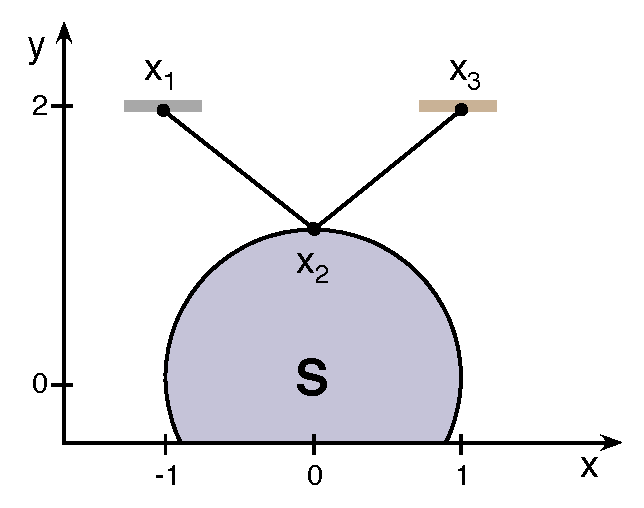
\includegraphics[width=0.4\textwidth]{figures/mlt/example}
	\caption{演示一个反射定律决定的局部约束函数,这里$\mathbf{x}_1$和$\mathbf{x}_3$的位置唯一决定了$\mathbf{x}_2$的位置}
	\label{f:mlt-example}
\end{figure}

那么,怎样利用当前路径的几何信息来求出该路径邻域内的约束函数呢?根据流形的性质,即它们在某个点的局部范围内满足一个唯一的映射关系,这个映射函数可由约束函数计算而得,所以约束函数实际上是对当前路径某个范围的邻域都有效的,为了表述每个顶点附近邻域内的当做变量的顶点,我们可以使用一阶泰勒展开来表述$C$的变量,即:

\begin{equation}
\begin{aligned}
	\mathbf{x}_i(u_i,v_i)&=\mathbf{x}_i+u_i({\rm \partial}_u\mathbf{x}_i)+v_i({\rm \partial}_v\mathbf{x}_i)\\
	\mathbf{n}_i(u_i,v_i)&=\mathbf{n}_i+u_i({\rm \partial}_u\mathbf{n}_i)+v_i({\rm \partial}_v\mathbf{n}_i)\\
	T(u_2,v_2)&=\begin{pmatrix}
		{\rm \partial}_u\mathbf{x}_2-\langle{\rm \partial}_u\mathbf{x}_2,\mathbf{n}_2(u_2,v_2)\rangle\mathbf{n}_2(u_2,v_2)\\
		{\rm \partial}_v\mathbf{x}_2-\langle{\rm \partial}_v\mathbf{x}_2,\mathbf{n}_2(u_2,v_2)\rangle\mathbf{n}_2(u_2,v_2)
	\end{pmatrix}
\end{aligned}
\end{equation}

在上式中,$u_i=v_i=0$即对应当前路径,$T(u_2,v_2)$表示用顶点$\mathbf{x}_2$相关的数据表示的正切空间,它仅与$\mathbf{x}_2$有关,将这些变量或项代入式\ref{e:mlt-example-c}就得到当前路径$\mathbf{x}_1\mathbf{x}_2\mathbf{x}_3$附近邻域内的约束函数$C$的形式,然后根据链规则就可以求各个导数,例如这里约束函数可以看做半矢量$h$和正切空间两项组成,对$C$的微分由两项组成:即一项保持半矢量$h$不变而求正切空间的导数,另一项保持正切空间不变而求半矢量的导数。对于前一项,即求$T$的导数可得:

\begin{equation}
\begin{aligned}
	\frac{T}{u_2}&=\begin{pmatrix}
		-\langle{\rm \partial}_u\mathbf{x}_2,{\rm \partial}_u\mathbf{n}_2\rangle\mathbf{n}_2-\langle{\rm \partial}_u\mathbf{x}_2,\mathbf{n}_2\rangle{\rm \partial}_u\mathbf{n}_2\\
		-\langle{\rm \partial}_v\mathbf{x}_2,{\rm \partial}_u\mathbf{n}_2\rangle\mathbf{n}_2-\langle{\rm \partial}_v\mathbf{x}_2,\mathbf{n}_2\rangle{\rm \partial}_u\mathbf{n}_2
	\end{pmatrix}\\
	\frac{T}{v_2}&=\begin{pmatrix}
		-\langle{\rm \partial}_u\mathbf{x}_2,{\rm \partial}_v\mathbf{n}_2\rangle\mathbf{n}_2-\langle{\rm \partial}_u\mathbf{x}_2,\mathbf{n}_2\rangle{\rm \partial}_v\mathbf{n}_2\\
		-\langle{\rm \partial}_v\mathbf{x}_2,{\rm \partial}_v\mathbf{n}_2\rangle\mathbf{n}_2-\langle{\rm \partial}_v\mathbf{x}_2,\mathbf{n}_2\rangle{\rm \partial}_v\mathbf{n}_2
	\end{pmatrix}
\end{aligned}
\end{equation}

\noindent 而对于第二项,也可以通过常规的导数计算规则得:

\begin{equation}
	\frac{{\rm \partial}}{{\rm \partial} t}\frac{\mathbf{z}(t)}{||\mathbf{z}(t)||}=\frac{1}{||\mathbf{z}(t)||}\frac{{\rm \partial}\mathbf{z}(t)}{||\mathbf{z}(t)||^{3}}\Bigg\langle\mathbf{z}(t),\frac{{\rm \partial}\mathbf{z}(t)}{{\rm \partial} t}\Bigg\rangle
\end{equation}

由此,我们可以借由顶点局部的特征信息(位置和法线导数)以及局部的参数表示构建出路径的局部约束函数,从而能够计算出路径中各个镜面顶点关于非镜面顶点的导数,这可以用于下一节的路径突变计算。

\cite{a:LIGHTTRANSPORTONPATHSPACEMANIFOLDS}计算出上述示例路径的雅可比矩阵为:

\begin{equation}
	\nabla C=\begin{bmatrix}
		-\frac{1}{4} & 0           & -\frac{3}{2} & 0  & \frac{1}{4} & 0 \\
		           0 & \frac{1}{2} & 0            & -1 & 0           & \frac{1}{2}
	\end{bmatrix}
\end{equation}

\noindent 因此可以得到正切空间:

\begin{equation}
	T_{\mathcal{S}}({\mathbf{x}})=-A^{-1}\begin{bmatrix}
		B_1 & B_2
	\end{bmatrix}=\begin{pmatrix}
		-\frac{1}{6} & 0 & \frac{1}{6} & 0\\
		0 & \frac{1}{2} & 0 &\frac{1}{2}
	\end{pmatrix}
\end{equation}

\noindent 以及泛化几何项:

\begin{equation}
	G(\mathbf{x}_1\leftrightarrow\mathbf{x}_3)=\bigg| P_2A^{-1}B_3\bigg|	G(\mathbf{x}_1\leftrightarrow\mathbf{x}_2)=\begin{vmatrix}
		\frac{1}{6} & 0\\
		0 & \frac{1}{2}	
	\end{vmatrix}G(\mathbf{x}_1\leftrightarrow\mathbf{x}_2)=\frac{1}{48}
\end{equation}

读者可以从\cite{a:LIGHTTRANSPORTONPATHSPACEMANIFOLDS,a:ManifoldExplorationExpanded}获得更多信息,其中还包含计算$\nabla C$相关的源代码,更具体的运用也可以参考\cite{m:MitsubaRenderer}中的源代码。





\subsubsection{流形上的行走}\label{sec:mlt-manifold-move}
现在,我们已经有了路径在流形上的表述,以及在局部区域内各个镜面顶点关于所有非镜面顶点的导数,此时如果我们对这些非镜面顶点执行某个突变增量,如$\Delta \mathbf{x}_1$和$\Delta \mathbf{x}_k$,则理论上我们可以得到所有镜面顶点在流形上的一个邻域中的位置,因此构成一个突变路径。

然而实际操作中没有这么简单,因为一个顶点局部邻域内的一阶泰勒近似可能并不位于该顶点所在的表面上,因此我们将寻求一些数学方法来辅助突变路径的计算。在数学中,利用一阶导数来逼近某个函数值的方法称为牛顿法,我们首先来简要介绍一下该方法的基本思路及原理。



\paragraph{牛顿方法}
牛顿法(Newton's method)\mathindex{牛顿法}{Newton's method}是一种数值方法,它通过一系列连续迭代的过程,寻找一个实数函数的根,即$x:f(x)=0$的近似值。

\begin{figure}
	\sidecaption
	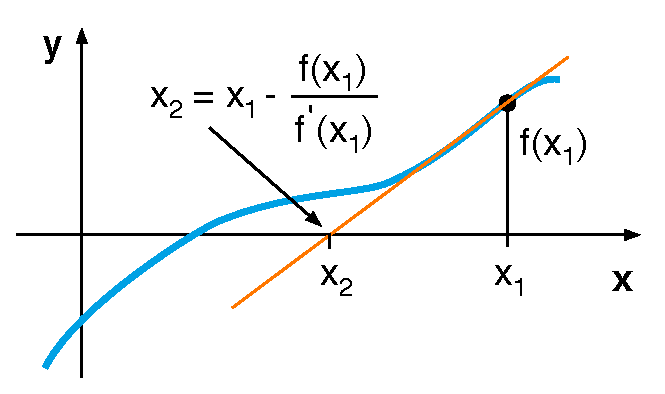
\includegraphics[width=0.5\textwidth]{figures/mlt/Newton-method}
	\caption{牛顿迭代法根据一阶泰勒近似对当前预测根计算一个更好的近似根,然后不断对该过程进行迭代,直到找到足够接近真实值的近似根}
	\label{f:mlt-Newton-method}
\end{figure}

给定一个定义域为实数$x$的函数$f$,该函数的导数$f^{'}$,以及任意一个初始的根的猜想值$x_1$,这里$f(x_1)\neq 0$(否则我们已经找到根了)。则根据一阶泰勒近似,$x_1$邻域内的函数曲线可以表示为$f(x_1+\epsilon)\approx f(x_1)+f^{'}(x_1)\epsilon$,这里所有$f(x_1+\epsilon)$的函数值位于函数在$x_1$点处的正切线上,如图\ref{f:mlt-Newton-method}所示。我们取该正切线与$x-$轴的交点$(x_1,0)$,这里设$x_1=f(x_0+\epsilon)$,则在满足该局部线性变换(一阶泰勒近似)的条件下,$x_1$相比$x_0$是函数$f(x)$的根的一个更好的近似。如果我们持续上述的过程,则可以得到更加接近于真实值的函数的根,在每个迭代中,新的预测位置$x_{n+1}$的值可以很容易求得为:

\begin{equation}
	x_{n_1}=x_n-\frac{f(x_n)}{f^{'}(x_n)}
\end{equation}

可以证明,牛顿法的收敛是呈二次方的(quadratic),即随着迭代过程逐渐收敛至函数的根,每个迭代中预测值与真实值之间的差异是呈二次方的:

\begin{equation}
	\Delta x_{i+1}=\frac{f^{''}(a)}{2f^{'}(a)}(\Delta x_i)^{2}+\mathcal{O}(\Delta x_i)^{3}
\end{equation}

\noindent 这里$a$表示函数的根的真实值,即$\lim\limits_{i\to\infty}x_i=a$,$\Delta x_i=x_i-a$表示预测值和真实值之间的差异。

牛顿法的收敛性及收敛速度依赖于一阶线性泰勒近似,例如当泰勒近似不能很好的反应函数在其切线与$x-$轴交点附近的分布时,可能导致错误的结果,或者初始预测值的范围过大,局部线性模型完全失去意义,此外当某些区域不能有效获取导数时也会导致不正确的结果。




\paragraph{流形行走算法}
我们可以借鉴牛顿法来实现流形上的行走。到目前为止,对于镜面流形我们已有的唯一基本工具就是所有镜面顶点相对于所有非镜面顶点的导数,然而直接通过导数计算一个一阶泰勒近似的路径并不是一条合法的路径,正如图\ref{f:mlt-Newton-method}中一阶近似的点$x_1$并不位于函数上一样,一阶近似路径中的顶点可能也完全不在流形上,因此我们需要使用类似牛顿法的方法使用一个迭代过程逼近一条真实的路径。

在上述的牛顿法中,每个迭代涉及两个基本的操作:首先,利用导数求出$x_n$邻域内点的一阶泰勒近似,并求出一个更好的近似值$x_{n+1}$(其为切线与$x-$轴的交点);然后,将该近似点$x_{n+1}$代入函数$f$中以求出下一迭代的导数$f^{'}(x_{n+1})$。对于镜面流形,我们已经具备第一个操作的计算能力,然而对于第二个操作,由于流形空间并不占据全部欧几里得空间,所以通过线性操作得到的路径并不能代入到下一迭代中进行使用,因此\cite{a:ManifoldExplorationAMarkovChainMonteCarloTechniqueforRenderingSceneswithDifficultSpecularTransport}使用了一个牛顿法的变体,即它添加了一种机制来将一个欧几里得空间线性变换的顶点映射回流形上面。

光线追踪提供了一种将表面外的顶点投射到表面上的方法,即已知$\mathbf{x}_1$和$\mathbf{x}_2$,其中$\mathbf{x}_2$位于表面外附近某一点(这里假设就是通过线性变换得到的近似点),可以通过向$\mathbf{x}_1\to\mathbf{x}_2$方向投射一条光线,然后找到该光线与表面的交点,从而将$\mathbf{x}_2$投射到表面。这样便能够对上述的一阶泰勒近似顶点进行“更正”,得到一个有效的路径顶点,从而最终得到一个有效的突变路径,如图\ref{f:mlt-manifold-walk}所示。

\begin{figure}
	\sidecaption
	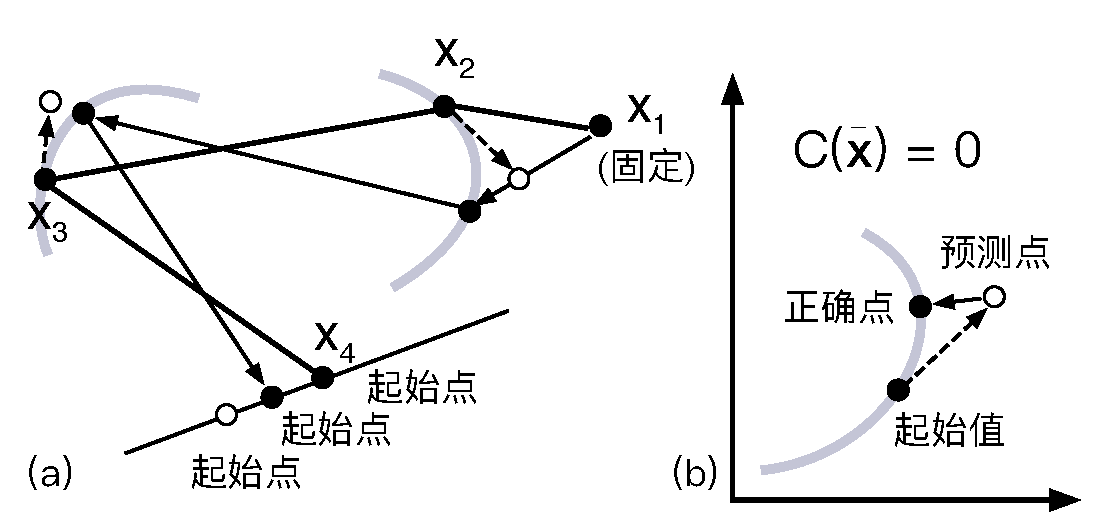
\includegraphics[width=0.65\textwidth]{figures/mlt/manifold-walk}
	\caption{我们将流形上的行走定义为流形探索的一个基本操作:它固定镜面路径的其中一个非镜面端点$\mathbf{x}_1$,然后指定另一个非镜面端点$\mathbf{x}_n$一个增量位置$\mathbf{x}^{'}_n$,最后我们使用类似牛顿迭代法寻找一条逼近该位置的路径}
	\label{f:mlt-manifold-walk}
\end{figure}

到此我们得到了使用一阶导数,以及类牛顿法计算一条突变路径的思路,接下来我们要定义什么是流形上的行走。除于后面会介绍的一些原因,我们不能仅仅是使用任意突变得到一条合法突变路径即可(否则我们不需要上述的牛顿迭代法),而是要得到一条满足指定条件的路径。更具体地,流形上的行走是指:对于一条长度为$n$的路径$\mathbf{x}_1,\cdots\mathbf{x}_n$,其中$\mathbf{x}_1$和$\mathbf{x}_n$为非镜面顶点,$\mathbf{x}_2,\cdots,\mathbf{x}_{n-1}$为镜面顶点,我们保持$\mathbf{x}_1$不变,而将$\mathbf{x}_n$调整到一个新的位置$\mathbf{x}^{'}_n$。

\begin{myshaded}
	为了与上面的牛顿法进行对比,考虑一个流形上的函数$f({\mathbf{x}})$,它的值为其末点$\mathbf{x}_n$的位置标量(例如这里可以取顶点位置矢量$\mathbf{x}_n$的模长得到一个标量,即$||\mathbf{x}_n||$)。对于给定顶点位置$||\mathbf{x}^{'}_n||$,我们的目标是要求$f({\mathbf{x}})-||\mathbf{x}^{'}_n||=0$的根。因此我们可以使用牛顿法来逼近得到这条近似路径,唯一的不同是我们需要借助光线追踪将欧几里得空间的近似路径投射回到流形上。
\end{myshaded}

有了前面这些分析,流形上的行走算法的思路就非常简单,\cite{a:ManifoldExplorationExpanded,a:LIGHTTRANSPORTONPATHSPACEMANIFOLDS}提供了该算法的基本步骤,如算法\ref{a:mlt-walk-manifold}所示,图\ref{f:mlt-manifold-walk}展示了相关的一些图示,我们以下对该算法做简要分析。

\begin{algorithm}
\begin{lstlisting}[language=C++, mathescape]
WalkManifold($\mathbf{x}_1,\cdots,\mathbf{x}_n\rightsquigarrow\mathbf{x}^{'}_n$)
	set $i = 0$ and $\beta = 1$
	while $||\mathbf{x}_n-\mathbf{x}^{'}_n||>\varepsilon L$
		$\mathbf{p} = \mathbf{x}_2 - \beta T(\mathbf{x}_2)P_2A^{-1}B_kT(\mathbf{x}_n)^{T}(\mathbf{x}^{'}_n-\mathbf{x}_n)$
		Propagate the ray $\mathbf{x}_1\to\mathbf{p}$ through all specular interactions, producing $\mathbf{x}^{+}_2,\cdots,\mathbf{x}^{n}_n$.
		if step 4 succeeded and $||\mathbf{x}^{+}_n-\mathbf{x}^{'}_n||<||\mathbf{x}_n-\mathbf{x}^{'}_n||$
			$\mathbf{x}_2,\cdots,\mathbf{x}_n=\mathbf{x}^{+}_2,\cdots,\mathbf{x}^{+}_n$
			$\beta=\min\{1,2\beta\}$
		else
			$\beta=\frac{1}{2}\beta$
		set $i=i+1$ and fail if $i>N$
	return $\mathbf{x}_2,\cdots,\mathbf{x}_{n-1}$
\end{lstlisting}
\caption{每个顶点存储的数据,其中位置,法线以及位置和法线的导数都是通过获取顶点的时候从表面表述中获得,而该顶点关于镜面流形的各个矩阵则通过微分几何相关的知识计算而得,并且这些矩阵的计算仅依赖于上述的顶点几何数据}
\label{a:mlt-walk-manifold}
\end{algorithm}

首先,该算法的目标是针对当前路径$\mathbf{x}_1,\cdots,\mathbf{x}_n$计算一条突变路径,使得起点$\mathbf{x}_1$保持不变,而终点为$\mathbf{x}^{'}_n$,这里很显然$\mathbf{x}^{'}_n$是个已知的输入参数。通过上述的分析可知,我们需要使用类牛顿法来得到一条近似的合法路径,算法中的while循环表示牛顿法的每个迭代,直到预测路径的终点$\mathbf{x}_n$非常逼近$\mathbf{x}^{'}_n$或者迭代次数大于$N$为止,这里$\epsilon L$即为无限接近的判断条件,取值$L=\max_i||\mathbf{x}_i||$和$\epsilon=10^{-7}$。

与传统的牛顿法不同的是,我们不能直接通过一阶泰勒近似得到一条合法的路径,所以这里仅对第2个顶点,即$\mathbf{x}_2$,使用线性模型得到一个预测顶点$\mathbf{p}$(如算法\ref{a:mlt-walk-manifold}第3行);然后后续的路径顶点将使用光线追踪的方式(如算法\ref{a:mlt-walk-manifold}第4行)计算而得,如图\ref{f:mlt-manifold-walk}所示,它首先对方向$\mathbf{x}_1\to\mathbf{p}$作光线投射,得到该光线与场景的交点,由于$\mathbf{x}_2,\cdots,\mathbf{x}_{n-1}$为镜面顶点,所以后续的光线传播按照镜面反射定律进行计算,这得到一条合法的预测路径为$\mathbf{x}^{+}_2,\cdots,\mathbf{x}^{+}_n$。如果该路径相对于当前路径其末点$\mathbf{x}^{+}_n$与目标末点$\mathbf{x}^{'}_n$的距离更加靠近,则在下一迭代中选择该路径为当前预测路径。需要注意的是,在上述的局部线性模型计算中,我们需要对每一条合法的预测路径计算约束函数的导数$\nabla C$及其相关矩阵,因为后续的迭代需要以这些路径为基础执行线性变换。

上述的计算方法虽然不是完全根据当前路径所有顶点的一阶线性变换来得出预测路径所有的顶点(而是只使用线性变换计算出第二个顶点$\mathbf{p}$,然后后续的顶点使用光线追踪得出),但是随着迭代的推进,线性近似模型越来越精确,它们仍然会收敛至正确的值。

$\beta$是一个用来调整牛顿迭代步幅的参数,它可以被动态的调整:当线性模型近似足够好时,它可以放心地增大迭代的步幅,否则减小迭代的步幅。

当预测路径足够逼近$\mathbf{x}^{'}_n$,上述算法返回最后的预测路径,注意这里$\mathbf{x}_{n-1}$与$\mathbf{x}^{'}_n$是直接连接的,即$\mathbf{x}^{+}_n$被抛弃。因此$\mathbf{x}^{+}_n$在迭代过程中仅仅是一个用来比较的中间变量,它的实际数值和几何无关紧要,因此我们可以虚构一个平面使$\mathbf{x}^{'}_n$和$\mathbf{x}_n$位于其中,如图\ref{f:mlt-manifold-walk}(a)所示,这简化了算法的实现。





\subsubsection{流形上的路径突变策略}\label{sec:mlt-manifold-perturbation}
上述的流形行走算法提供了一种基于一条镜面流形路径,得到一条突变路径的能力,然而这还不能使其成为一个完整的路径突变策略,例如它对于包含多(大于2)个非镜面顶点的路径无法处理,虽然理论上我们可以对任意路径按照上述的方法进行类似推算,但是多个相关的漫反射顶点(相当于多元函数)会使得计算非常复杂;此外,镜面流形行走只是关于小步幅的突变,这样将导致很难快速在全局图像空间进行收敛。

所以,\cite{a:ManifoldExplorationAMarkovChainMonteCarloTechniqueforRenderingSceneswithDifficultSpecularTransport}只是将上节中的流形行走算法当做一种最基本且最简单的单元操作,一个完整的流形突变策略可能会对其中的某一部分镜面子路径执行镜面流形行走算法,但是流形突变算法本身还包括如多漫反射顶点处理,满足全局遍历性等特性。

为了能够以更高的接受概率,以及对更大范围内不同类型的路径进行修改,\cite{a:ManifoldExplorationAMarkovChainMonteCarloTechniqueforRenderingSceneswithDifficultSpecularTransport}的流形突变算法结构与\cite{a:MetropolisLightTransport}中的路径突变算法有些类似,即首先随机选择当前路径中需要修改的某个子路径,然后对该子路径执行突变操作。但流形突变算法中每个部分存在很多不同,例如待修改的路径不是以长度为依据选择的,它也不要求修改过的子路径与原路径的连接处包含两个漫反射顶点,此外,流形突变的子路径修改包含了使用流形行走算法,接受概率更高。我们将在下面的详细介绍中看到这些不同点。

\begin{figure}
	\sidecaption
	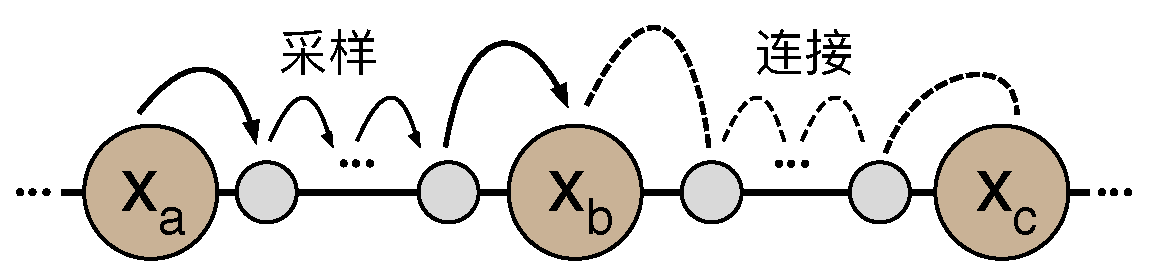
\includegraphics[width=0.65\textwidth]{figures/mlt/manifold-perturbation}
	\caption{流形路径突变策略包含一个采样阶段和一个连接阶段}
	\label{f:mlt-manifold-perturbation}
\end{figure}

具体地,流形路径突变算法可以分为两个不同的阶段:即采样阶段和连接阶段,如图\ref{f:mlt-manifold-perturbation}所示。在采样阶段,算法首先随机选择包含三个漫反射顶点$\mathbf{x}_a,\mathbf{x}_b$和$\mathbf{x}_c$的子路径,很显然该子路径有可能会被一些镜面顶点分离,接着算法再对顶点$\mathbf{x}_a$随机选择一个突变方向并沿着可能的镜面路径传播直到到达顶点$\mathbf{x}_b$附近的一个非镜面顶点$\mathbf{x}^{'}_b$,如果$\mathbf{x}^{'}_b$和$\mathbf{x}_b$属于不同的表面则该突变直接被拒绝;否则进入连接阶段,这里使用前面讲述的流形行走算法“连接”顶点$\mathbf{x}^{'}_b$和$\mathbf{x}_c$。图\ref{f:mlt-manifold-perturbation-example}包含了一个流形突变的示例,以下我们对各个阶段进行详细描述。

\begin{figure}
	\sidecaption
	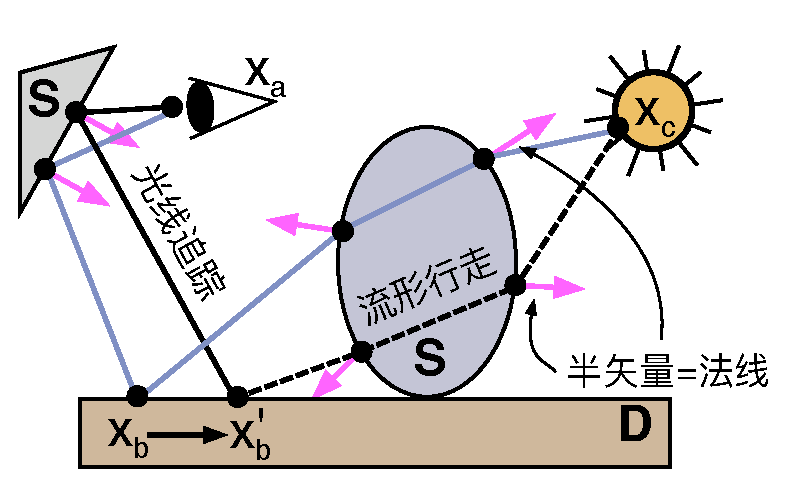
\includegraphics[width=0.45\textwidth]{figures/mlt/manifold-perturbation-example}
	\caption{流形突变对顶点$\mathbf{x}_a$的方向做一个微小突变,然后沿此方向使用光线追踪的方式进行传输,直至到达$\mathbf{x}_b$附近的一点$\mathbf{x}^{'}_b$;传统的方法并不知道怎么连接$\mathbf{x}^{'}_b$和$\mathbf{x}_c$,而流形行走提供了一种经过多个镜面反射连接$\mathbf{x}^{'}_b$和$\mathbf{x}_c$的方法}
	\label{f:mlt-manifold-perturbation-example}
\end{figure}




\paragraph{采样阶段}
首先需要注意,采样阶段实际上包含两种采样,即首先对$\mathbf{x}_a,\mathbf{x}_b$和$\mathbf{x}_c$三个顶点组成的子路径选择的采样,其次是对顶点$\mathbf{x}_a$传输方向的采样。

对于子路径$\mathbf{x}_a,\cdots,\mathbf{x}_b,\cdots,\mathbf{x}_c$的选择,它首先从路径中均匀随机地选择一个非镜面顶点$\mathbf{x}_a$以及一个突变方向(比如是向摄像机或光源方向进行突变),然后按方向遍历路径中的顶点直到找到$\mathbf{x}_b$和$\mathbf{x}_c$,这个过程有可能失败,如果查找失败则重新进行选择。在后续的子路径修改中,不管该子路径是什么方向,我们假设$a<b<c$。

对于$\mathbf{x}_a$突变方向的采样,它的目的是通过对子路径$\mathbf{x}_{a+1},\cdots,\mathbf{x}_b$产生突变得到一条“近邻”路径$\mathbf{x}^{'}_{a+1},\cdots,\mathbf{x}^{'}_b$。设顶点$\mathbf{x}_a$散射的入射和出射方向分别为$\omega_i=\overrightarrow{\mathbf{x}_a\mathbf{x}_{a-1}}$和$\omega_o=\overrightarrow{\mathbf{x}_a\mathbf{x}_{a+1}}$,$\mathbf{x}_a$的方向突变通过对一个围绕方向$\omega_o$的球形分布$D(\omega^{'}_o)$进行采样,并通过光线追踪决定顶点$\mathbf{x}^{'}_{a+1}$的位置,直至达到$\mathbf{x}^{'}_b$。

为了使突变路径$\mathbf{x}^{'}_{a+1},\cdots,\mathbf{x}^{'}_b$具有较高的接受率,且能够适应顶点$\mathbf{x}_a$的散射特征,方向分布$D(\omega^{'}_o)$必须满足两个条件:首先是该方向分布必须以方向$\omega_o$为中心,因为$\mathbf{x}^{'}_{a+1}$点为镜面顶点,因此较大的方向突变会导致较大的路径突变;其次,该方向分布随着顶点$\mathbf{x}_a$的BRDF系数的变化而变化,例如当顶点$\mathbf{x}_a$在比较粗糙的表面上时,方向分布$D(\omega^{'}_o)$更可能产生比较大的突变,而对于光泽表面,较大的突变方向则总是会被拒绝。\cite{a:ManifoldExplorationAMarkovChainMonteCarloTechniqueforRenderingSceneswithDifficultSpecularTransport}对该方向函数使用冯·米泽斯-费雪分布(Von Mises–Fisher distribution)\cite{b:Directionalstatistics,b:Statisticalanalysisofsphericaldata}来描述,该分布以方向$\omega_o$为中心,且中心方向的概率$D(\omega_o=\lambda^{2}p(\omega_i\to\omega_o))$,其实$p(\omega_i\to\omega_o)$表示顶点$\mathbf{x}_a$处对BRDF分布进行重要性采样的概率,$\lambda$表示一个用户控制参数(这也是流形探索比较主要的控制参数),通常取值50到100之间。

当$\mathbf{x}_a$处于摄像机或者光源上时,为了使突变均匀分布于图像空间或光源面积上,\cite{a:ManifoldExplorationAMarkovChainMonteCarloTechniqueforRenderingSceneswithDifficultSpecularTransport}采用了\cite{a:MetropolisLightTransport}中类似的策略,将摄像机顶点和光源顶点表述为两个顶点,即在每个长度为$k$的全路径的两端分别添加一个无状态的顶点$\mathbf{x}_0$和$\mathbf{x}_{k+1}$,这两个顶点没有位置状态,称为一个伪顶点或超顶点,它们的方法分布为摄像机或光源上面积的均匀分布,这样摄像机顶点和光源顶点可以当做传统的顶点处理,且$\mathbf{x}_a$可以在图像空间或光源面积上均匀分布。




\paragraph{连接阶段}
上述的采样阶段涉及随机采样的过程,而接下来的连接阶段则是一个确定性的计算过程。

如果$\mathbf{b}^{'}_b$和$\mathbf{x}_c$之间不包含镜面顶点,则它们之间的连接仅涉及可见性的判断,这是两个漫反射顶点之间的连接;当它们之间存在镜面顶点时,我们需要使用前面讨论的流形行走来连接顶点$\mathbf{b}^{'}_b$和$\mathbf{x}_c$:

\begin{equation}
	\mathbf{x}^{c-1},\cdots,\mathbf{x}^{'}_{b+1}=\text{WalkManifold}(\mathbf{x}_c,\cdots,\mathbf{b}\to\mathbf{x}^{'}_b)
\end{equation}

最后我们仍然需要判断$\mathbf{b}^{'}_b$和$\mathbf{x}_c$之间的可见性(这是因为前面流形行走算法仅把$\mathbf{x}^{+}_n$看做一个虚拟顶点)。



\paragraph{转移概率}
梅特波利斯算法要求状态之间的转移是可逆的,即状态之间的相互转移概率必须同时满足$T(\mathbf{x},\mathbf{x}^{'})>0$和$T(\mathbf{x}^{'},\mathbf{x})>0$,这给流形行走带来了一个问题:因为流形行走算法可能是不可逆的。例如即使$\mathbf{x}$能够转移至$\mathbf{x}^{'}$,但由$\mathbf{x}^{'}$向$\mathbf{x}$的转移却可能失败;其次,即使$\mathbf{x}^{'}$能够收敛至$\mathbf{x}$,但它构成的转移路径可能具有不同的几何配置(例如某些顶点穿过了不同物体的表面)。

为了避免这个问题,流形探索算法会对收敛的突变路径作反向的流形行走,如果反向的流形行走失败,则该突变路径被抛弃。

最终,流形突变路径的接受概率为:

\begin{equation}
	a({\mathbf{x}},{\mathbf{x}}^{'})=\min\bigg\{1,\frac{f_i({\mathbf{x}}^{'})T({\mathbf{x}}^{'},{\mathbf{x}})}{f_i({\mathbf{x}})T({\mathbf{x}},{\mathbf{x}}^{'})}\bigg\}
\end{equation}

\noindent 这里$T(\mathbf{x},\mathbf{x}^{'})$和$T(\mathbf{x}^{'},\mathbf{x})$表示正向和反向流形探索的转移概率,它们主要涉及对$\mathbf{x}_a$的突变方向$\omega^{'}_o$的采样概率。与传统的基于方向的光照积分方程到基于路径的光照积分方程的转变相似,由于对$D(\omega^{'}_o)$的采样结果是一个方向,这里需要执行一个方向到面积的变量替换,即立体角与该立体角到面积的投影的比值,所以最终的转移概率为$D^{\perp}(\omega^{'}_o)F(\mathbf{x}_a)\leftrightarrow\cdots\leftrightarrow\mathbf{x}^{'}_b$,这里第二项为泛化几何项,因为它可能涉及镜面路径的传播,它们可以通过约束函数的雅可比矩阵求得。





\subsubsection{扩展至光泽表面}\label{sec:mlt-manifold-specular}
上述的流形探索仅包含对理想镜面流形的探索,在这种情况下,所有镜面反射可以根据反射或折射定理约束,使其镜面顶点可以被局部表述为其他非镜面顶点的函数,从而实现对欧几里得路径空间的降维,然后在低维的流形空间进行处理。

对于镜面反射或折射,入射方向和反射方向构成的半矢量与镜面的法线重合。考虑到根据微面元BRDF理论,对于光泽表面,半矢量虽然可能与宏观的表面法线并不重合,但是它却可以看做和微面元的法线是重合的,为此我们可以将反射和折射定理的约束方程作用于光泽表面,只不过这里半矢量到表面宏观法线的投影不再是零矢量,而是一个常数,但是常数的导数仍然为0,所以\cite{a:ManifoldExplorationAMarkovChainMonteCarloTechniqueforRenderingSceneswithDifficultSpecularTransport}据此思路将流形探索扩展到光泽表面。

然而,尽管光泽流形的表述和导数计算没有太大变化,光泽流形的光照贡献函数$f$和其路径表述却不再处于相同的空间,因为这里虽然光泽顶点通过使用半矢量代替法线仍然能够减少路径空间的维度从而得到镜面流形空间,然而BRDF系数却不再是一个(由反射定律或折射定理唯一决定的)常数,它回到了原始的函数状态,并且其维度随着路径中镜面顶点数量的变化而变化,所以光照贡献函数$f$处于比光泽流形(原始的镜面流形空间$\mathcal{S}$)更高的维度,因此必须要涉及变量替换等辅助的操作。

\cite{a:TheNaturalConstraintRepresentationofthePathSpaceforEfficientLightTransportSimulation}受此思路的启发,提出了一个全新的完全基于半矢量空间的光照传输技术,它能够覆盖\cite{a:ManifoldExplorationAMarkovChainMonteCarloTechniqueforRenderingSceneswithDifficultSpecularTransport}中对光泽流形的扩展,并且具有更加直观的表述和完整的理论,它能够同时处理光泽表面和镜面表面,因此我们将这部分内容放入到下一节进行讨论。





\subsection{半矢量空间光照传输}\label{sec:mlt-hslt}
首先让我们再简要地总结一下关于流形探索的思路。传统的路径采样是完全随机的,这里的随机可以理解为采样器不会考虑任何关于场景的几何特征而“盲目的”在路径空间行走;因此,对于那些存在于很小的区域,但是被积函数的贡献值非常大的“困难”路径,往往会由于采样概率非常低而使其估计不精确;虽然MLT算法引入了路径之间的相关性,但是本质上它只是通过限制一条突变路径各个顶点的取值在欧几里得空间的某个范围内,其使用的路径采样(例如双向路径采样)仍然是盲目的,其效率仍然非常低;然而MLT算法提供了一种绝对的优势,即一旦找到一条重要路径,我们可以更小心地探索该路径附近也可能具有同样重要性的路径。

要想有效地探索这些困难路径,则必须了解并利用路径的一些局部几何信息,这是前面流形探索以及本节半矢量空间光照传输的核心内容。然而,要想让路径采样器\footnote{这里的路径采样器是指传统的根据光线追踪的路径采样,它几乎也是目前我们介绍的以及离线渲染中使用的唯一的路径采样器。}直接能够感知整个场景中的几何信息显然是不可能的,因为光线追踪依赖于首先随机选择一个方向,然后对该方向使用光线投射来寻找其与表面的交点并取得几何数据,而不是先根据某种场景的几何特征选择一个方向。

这种不可能事先知道场景几何特征的采样方法,使得我们转向另一种思路:即首先通过传统的路径追踪得到一条随机的合法路径,然后提取出该路径的几何特征,进而利用这些几何特征来寻找一条该路径附近的路径。这种思路依赖于一条已知路径,显然它不能成为一种独立的路径采样方法,然而它却正好可以用在MLT算法中,因为MLT算法寻找一条相对于当前路径的突变路径。然而需要注意的是,局部特征的表述的精确性往往被限定在很小的局部范围(如前面镜面流形表述所描述的那样),因此这些算法必须很好地保证全局遍历性的要求。

那么,应该怎样提取一条合法路径的局部几何信息呢,费马定理提供了答案。1657年,费马提出著名的最小时间原理,即自然界的行为永远以路程最短为原则。按照这个原理,光永远是选这样一条路走,以使它在最短时间内抵达目的地,这就是费马定理(Fermat principle)\myindex{费马定理}{Fermat principle}。费马定理描述了光照传输的特征,如果已知一条合法的光线路径,它当然满足费马原理,因此可以从中提取与光照交互有关表面的几何信息。

然而费马原理是全局的,它用于描述一条完全的路径,直接推导出这种全路径与多个表面交互的关系是非常困难的。幸运的是,局部的反射定律和折射定理与费马定理是完全等效的,局部的反射和折射定理提供了路径顶点及方向关于这些顶点局部几何信息(如位置,法线以及这些量的导数)的关系,从而我们能够从一条已知路径推导出该路径的局部几何信息。

然后,已知了一条路径的局部几何信息了,该如何利用它们来产生一条“相似”路径呢,这时牛顿方法提供了答案。我们已知的顶点局部信息是关于对应表面在该顶点处的位置和法线关于局部坐标系的导数,导数能够被运用于一阶泰勒近似中用来表述局部的函数分布,然而这种近似不能直接用来作为采样值,我们需要精确值,而牛顿方法正是利用一阶导数用迭代的方式逼近某个设定的真实函数值。

于是我们能够通过一条已知路径获得一条“相似”或“近邻”路径,这条路径在MLT算法中具有较高的接受率,因为它探索了路径的局部几何特征。更为重要的是,上述的采样过程是确定性的:给定一条当前路径,我们没有依赖任何随机过程,而是使用微分几何相关的知识直接计算出一条“相似”路径,这种由随机向确定性的转变,提升了MLT算法的效率。




\subsubsection{路径的空间}
半矢量光照传输中的路径采样作用于一个被称为半矢量空间的作用域,又称为自然约束空间,所以为了理解半矢量光照传输相关的概率及方法,我们首先来介绍路径采样发生的各种坐标空间,它们各自的优缺点以及各个空间之间的相互转换。

传统的光照传输的计算大多数基于路径形式的积分\cite{a:RobustMonteCarloMethodsforLightTransportSimulation},第$j-$个像素的贡献值$I_j$等于其测量贡献函数$f_j({\mathbf{x}})$在一个面积乘积形式${\rm d}\mathbf{X}$上的积分:

\begin{equation}
	I_j={\rm \int}_{\Omega}f_j(\mathbf{X}){\rm d}\mathbf{X}, \text{ 其中: } {\rm d}\mathbf{X}\equiv \prod^{k}_{i=0}{\rm d}A(\mathbf{x}_i)
\end{equation}

\noindent 这里$\Omega$表示路径空间,路径是一个通过场景中物体上多个交互顶点$\mathbf{x}_i$连接光源$\mathbf{x}_0$和摄像机$\mathbf{x}_k$的一条路径$\mathbf{X}=(\mathbf{x}_0,\cdots,\mathbf{x}_k)$。上式似乎说明我们可以通过对场景随机抽取$k+1$个顶点构成一条路径,然而前面已经分析过,由于顶点之间的连接必须满足可见性和顶点的BRDF分布等条件,随机选择的路径通常是不合法的,我们对路径的采样是使用光线追踪的方式,即对顶点$\mathbf{x}_i$的BRDF分布采样一个方向并通过光线投射决定下一个顶点$\mathbf{x}_{i+1}$的位置。

由此,由顶点的出射方向的立体角构成的作用域${\rm d}\mathbf{o}$似乎是一个更自然的选择,然而这种选择会带来麻烦。因为人眼或摄像机感知的量是辐射亮度$L$,它表示单位时间内穿过单位面积的光的密度,如果使用${\rm d}\mathbf{o}$作为积分空间,我们不得不考虑接受光照表面面积的大小。因此我们何不设定所有顶点$\mathbf{x}_i$接受光照的表面面积始终为单位面积,这就是光照传输的路径积分形式。然而我们的路径是从立体角作用域采样而得的,因此这就涉及一个由立体角${\rm d}\mathbf{o}$向表面面积${\rm d}A$(由于这里设定为单位面积,因为面积的概念被弱化,一块接受面积可以仅使用一个顶点${\rm d}\mathbf{x}$代替)的变量替换,根据立体角的概念可以得到:

\begin{equation}
	G(\mathbf{x}_i,\mathbf{x}_{i+1})=\Bigg|
		\frac{{\rm d}\mathbf{o}^{\perp}_{i}}{{\rm d}\mathbf{x}_{i+1}}
	\Bigg|=\Bigg|
		\frac{{\rm d}\mathbf{o}_i\langle\mathbf{o}_i,\mathbf{n}_i\rangle}{{\rm d}\mathbf{x}_{i+1}}
		\Bigg|=\frac{|\langle\mathbf{i}_{i+1},\mathbf{n}_{i+1} \rangle\langle\mathbf{o}_i,\mathbf{n}_i\rangle |}{||\mathbf{x}_i-\mathbf{x}_{i+1}||^{2}}
\end{equation}

我们称该变量替换的雅可比行列式为一个几何项(geometric term)\myindex{几何项}{geometric term},所有顶点$\mathbf{x}_i$向$\mathbf{x}_{i+1}$的传输形成的几何项的乘积,以及所有顶点BRDF系数等构成了上述的测量贡献函数$f(\mathbf{X})$,它也是我们需要对一条路径计算的光照贡献值,不管使用什么样的空间对路径进行采样(例如上一节在流形上对路径进行采样),最终都需要变换到路径空间进行光照贡献值的计算。

以上,我们已经介绍了路径的两种不同的空间及其变换,大多数的路径采样都是通过光线追踪的方式对立体角空间采样\footnote{注意,原采样空间也是基于立体角的空间,因此继承相同的缺点。},然后变换到路径空间,这种方式的缺点是光线投射无法控制和预测后续顶点的位置,因此不适合用于MLT算法进行路径突变。此外,由立体角向面积变量替换形成的几何项包含奇点值,即当两相邻顶点距离很小时,贡献值函数的值将无限大,使得被积函数的频率变化很大,我们将在后面看到半矢量空间的表述使得被积函数非常平滑。

上一节由费马定理出发推导出路径的局部约束,这使得我们可以很轻易地探索一条已知路径的局部区域,以寻找一条“相似”路径,然而它仅适用于镜面流形,\cite{a:TheNaturalConstraintRepresentationofthePathSpaceforEfficientLightTransportSimulation}受此启发提出能够有效处理光泽表面的半矢量空间光照传输。

在流形探索中,一个局部的镜面反射可以建立一个满足反射或折射定理的局部约束函数,这通过使入射光和出射光构成的半矢量与该顶点的法线重合来实现。为了处理光泽表面,考虑在微面元BRDF理论中,每个微面元可以被看做是绝对光滑的,因此我们可以在微面元上建立起上述类似的约束,然而与镜面流形不同的是,微面元使用的半矢量并不与宏观表面顶点的法线重合,但是微面元和宏观顶点之间通过微面元BRDF理论建立起了联系,因此这种微面元的约束被作用于宏观顶点之上,这样顶点$\mathbf{x}_i$处的半矢量$\mathbf{h}_i$能够充当任意一个光泽顶点的约束,我们称这样的约束为自然约束(natural constraint)\myindex{自然约束}{natural constraint},因此一条路径可以表述为:

\begin{equation}\label{e:mlt-half-vector-space}
	\mathbf{H}^{\perp}=(\mathbf{x}_0,\mathbf{h}^{\perp}_1,\mathbf{h}^{\perp}_2,\cdots,\mathbf{h}^{\perp}_{k-1},\mathbf{x}_k)\in\Omega(\mathbf{h}^{\perp})\subset\Omega
\end{equation}

这里将路径的首尾两个顶点$\mathbf{x}_0$和$\mathbf{x}_k$保留在原空间,符号$\perp$表示投影,例如$\mathbf{h}^{\perp}_i$表示投影的半矢量,$\mathbf{H}^{\perp}$表示投影(到顶点的局部坐标系下)的半矢量空间(projected half vector space)\myindex{投影的半矢量空间}{projected half vector space},或者称为自然约束空间(space of natural constraints)\myindex{自然约束空间}{space of natural constraints}。

以下先对半矢量空间进行分析,然后介绍基于半矢量空间的路径突变策略。





\subsubsection{半矢量空间}\label{sec:mlt-half-vector-space}
在使用这个新的路径空间进行采样(基于当前路径的突变)之前,需要弄清楚几件事情:首先是半矢量空间到原路径空间的变换(因为需要在路径空间计算路径的光照贡献值),这通过求解变量替换的雅可比矩阵的行列式来实现;因此,其次的问题是怎样求解半矢量空间到路径空间变量替换的雅可比矩阵;此外,我们还能通过推导出的空间变化法线半矢量空间的一些属性特征。

根据光照的路径积分方程,由半矢量空间向路径空间的变换可表示为:

\begin{equation}
	{\rm \int}_{\Omega(\mathbf{x}_0)}f(\mathbf{X}){\rm d}\mathbf{X}={\rm \int}_{\Omega(\mathbf{H}^{\perp}_{0})}f(\mathbf{X})\Bigg|\frac{{\rm d}\mathbf{X}}{{\rm d}\mathbf{H}^{\perp}}\Bigg| {\rm d}\mathbf{H}^{\perp}
\end{equation}

\noindent 这里$\Omega(\mathbf{x}_0)$和$\Omega(\mathbf{H}^{\perp}_{0})$表示路径空间中位于路径$\mathbf{X}_0$附近的一个子空间(对于半矢量空间是一个流形),并使得半矢量空间中子流形(每个顶点对应的半矢量约束描述的流形)中的半矢量满足顶点的局部参数化表述,因为半矢量表述的自然约束仅针对局部区域有效,这与镜面流形类似。

对于原始路径空间的被积函数$f(\mathbf{X})$,它实际上已经包含立体角向面积变换的雅可比行列式,即几何项$G$,所以上式中基于半矢量空间的被积函数可以写为:

\begin{equation}\label{e:mlt-change-of-variables}
	f(\mathbf{X})\Bigg|\frac{{\rm d}\mathbf{X}}{{\rm d}\mathbf{H}^{\perp}}\Bigg|=\rho(\mathbf{X})\Biggl(\prod^{k-1}_{i=0}G(\mathbf{x}_i,\mathbf{x}_{i+1})\Biggl)\Bigg|\frac{d(\mathbf{x}_1\cdots\mathbf{x}_{k-1})}{d(\mathbf{h}^{\perp}_1\cdots\mathbf{h}^{\perp}_{k-1})}\Bigg|
\end{equation}

\noindent 其中,$\rho(\mathbf{X})$是$f(\mathbf{X})$中除几何项以外的所有项(例如所有顶点BRDF函数的乘积),由于这些项不受空间变换的影响,在以下的分析中将被忽略。第二个雅可比行列式表示半矢量空间向路径空间的变换,在我们现有的知识中并不包含对这个变换的介绍,我们将对上式进行一定的变换,以寻找新的变换关系。

给定式\ref{e:mlt-half-vector-space}表示的路径,对式\ref{e:mlt-change-of-variables}除以不变项$\rho$并做适当的变换可得:

\begin{equation}\label{e:mlt-half-vector-jacobians}
\begin{aligned}
	\text{式\ref{e:mlt-change-of-variables}}/\rho(\mathbf{X})&=\Biggl|\frac{d(\mathbf{o}^{\perp}_0\cdots\mathbf{o}^{\perp}_{k-1})}{d(\mathbf{x}_1\cdots\mathbf{x}_k)}\Biggl|\Biggl|\frac{d(\mathbf{x}_1\cdots\mathbf{x}_{k-1})}{d(\mathbf{h}^{\perp}_1\cdots\mathbf{h}^{\perp}_{k-1})}\Biggl|\\
	&=\Biggl|\frac{d(\mathbf{o}^{\perp}_0,\mathbf{o}^{\perp}_1\cdots\mathbf{o}^{\perp}_{k-1})}{d(\mathbf{x}_k,\mathbf{x}_1\cdots\mathbf{x}_{k-1})}\Biggl|\Biggl|\frac{d(\mathbf{x}_1\cdots\mathbf{x}_{k-1})}{d(\mathbf{h}^{\perp}_1\cdots\mathbf{h}^{\perp}_{k-1})}\Biggl|\\
	&=\Biggl|\frac{{\rm d}\mathbf{o}^{\perp}_0}{{\rm d}\mathbf{x}_k}\Biggl|\prod^{k-1}_{i=1}\Biggl|\frac{{\rm d}\mathbf{o}_i}{{\rm d}\mathbf{h}_i}\Biggl|\Biggl|\frac{\langle\mathbf{o}_i,\mathbf{n}_i\rangle}{\langle\mathbf{h}_i,\mathbf{n}_i\rangle}\Biggl|
\end{aligned}
\end{equation}

\noindent 这里首先对第一个行列式执行一系列列变换,以及根据导数的链规则(即:$(f\cdot g)(a)=f^{'}(g(a))g^{'}(a)$)和行列式的性质(即:$\det(AB)=\det(A)\det(B)$)进行重新整理。式\ref{e:mlt-half-vector-jacobians}中的第一项正是上一节中介绍的对于镜面链泛化几何项:

\begin{equation}
	\Biggl|\frac{{\rm d}\mathbf{o}^{\perp}_0}{{\rm d}\mathbf{x}_k}\Biggl|=\Biggl|\frac{{\rm d}\mathbf{o}^{\perp}_0}{{\rm d}\mathbf{x}_1}\Biggl|\Biggl|\frac{{\rm d}\mathbf{x}_1}{{\rm d}\mathbf{x}_k}\Biggl| =G(\mathbf{x}_0,\mathbf{x}_1)|T_1|	
\end{equation}

由于半矢量空间的变换是基于微面元表面绝对光滑的假设建立的局部约束,所以这里的路径可以看做满足镜面链的条件(外加微面元到宏观顶点的关系来描述光泽特性,下面分析),因此这里可以完全使用镜面流形探索相同的方法来计算泛化几何项$G$以及局部坐标变换$T_1$。在计算的时候唯一的区别是,由于半矢量并不与顶点的法线重合,因此约束函数右边项不是一个常数,但是其导数仍然为0,所以这并不影响式\ref{e:mlt-half-vector-jacobians}中第一项的计算。

\begin{figure}
	\sidecaption
	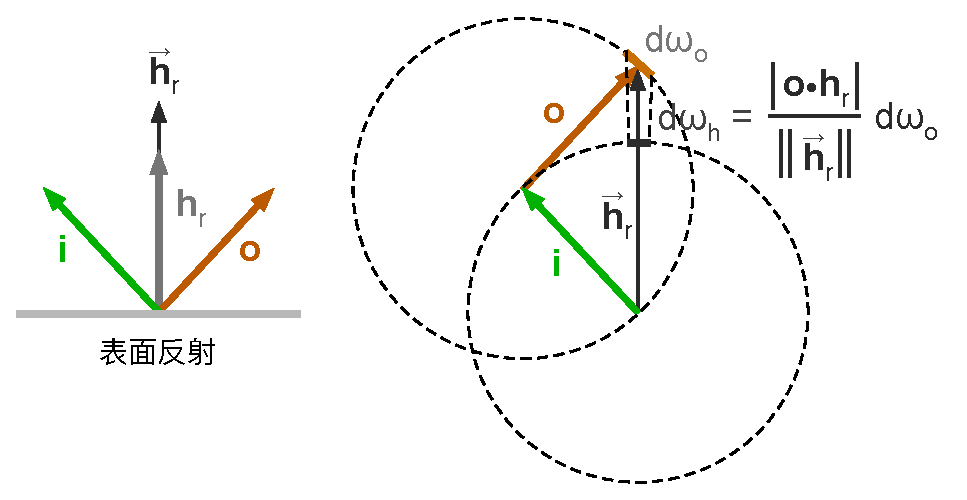
\includegraphics[width=0.65\textwidth]{figures/mlt/half-vector}
	\caption{在微面元BRDF理论中,半矢量相对于出射方向立体角的雅可比行列式可以通过图示的几何关系求得:即出射方向立体角的增量引起的半矢量方向的增量在单位圆形上的投影面积}
	\label{f:mlt-half-vector}
\end{figure}

而式\ref{e:mlt-half-vector-jacobians}中的第二项,即顶点出射立体角相对于顶点半矢量的雅可比行列式,可以通过微面元BRDF理论\cite{a:RobustMonteCarloMethodsforLightTransportSimulation}计算而出,为了理解的连贯性,我们这里给予简单说明。如图\ref{f:mlt-half-vector}所示(这里仅针对镜面反射给予说明,镜面折射请参考原论文中的描述)镜面反射几何关系,这里半矢量$\vec{\mathbf{h}}_r = \mathbf{i} + \mathbf{o}$, 而$\mathbf{h}_r = \vec{\mathbf{h}}_r / ||\vec{\mathbf{h}}_r||$表示归一化的半矢量,为了计算雅可比行列式,我们对出射方向使用一个增量${\rm d}\omega_o$,它将导致半矢量方向的一个增量${\rm d}\omega_h$,该增量的大小等于其在单位圆上的投影面积。

所以很容易计算出将半矢量密度转换为出射方向的雅可比行列式为:

\begin{equation}
	\Bigg|\frac{{\rm d}\mathbf{h}}{{\rm d}\mathbf{o}}\Bigg|=\frac{\eta^{2}|\langle\mathbf{h},\mathbf{o}\rangle|}{(\langle\mathbf{h},\mathbf{i}\rangle+\eta\langle\mathbf{h},\mathbf{o}\rangle)^{2}}
\end{equation}

这里$\eta$表示入射方向介质折射率$\eta_o$与入射方向介质折射率$\eta_i$的比值$\eta_o/\eta_i$,将上式代入式\ref{e:mlt-half-vector-jacobians}可以得到:

\begin{equation}\label{e:mlt-half-vector-space-jacobian}
	=\Biggl|\frac{{\rm d}\mathbf{o}^{\perp}_0}{{\rm d}\mathbf{x}_k}\Biggl|\prod^{k-1}_{i=1}\frac{(\langle\mathbf{h},\mathbf{i}\rangle+\eta\langle\mathbf{h},\mathbf{o}\rangle)^{2}}{\eta^{2}|\langle\mathbf{h},\mathbf{o}\rangle|}
\end{equation}

因此,式\ref{e:mlt-half-vector-jacobians}可以看做首先将$\mathbf{x}_0$的出射立体角转换为$\mathbf{x}_k$上的面积密度,这是一个泛化几何项,这一步将整个路径看做一个镜面链,因此这个泛化几何项表现为镜面流形上的一个转移矩阵(见第\ref{sec:mlt-me}节的内容);然后再对每个顶点执行半矢量向出射方向的变换以考虑顶点的光泽度,如图\ref{f:mlt-half-vector-space-jacobians}所示。

\begin{figure}
	\sidecaption
	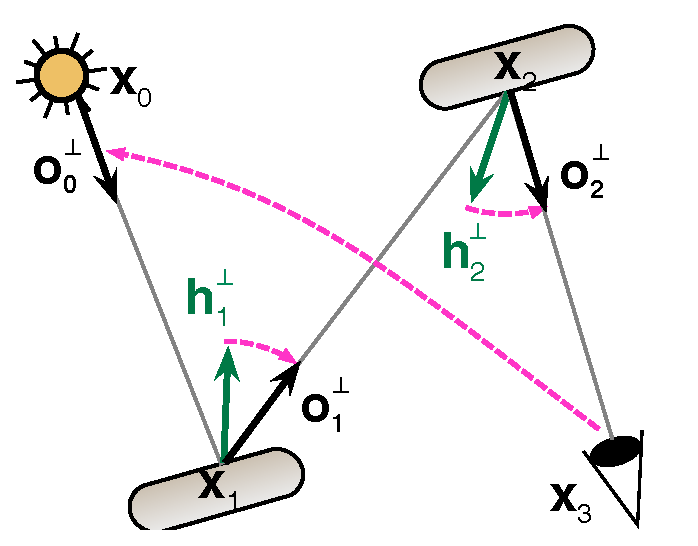
\includegraphics[width=0.4\textwidth]{figures/mlt/half-vector-space-jacobians}
	\caption{式\ref{e:mlt-half-vector-space}表示的半矢量空间相对于路径空间的雅可比行列式可以看做是两个行列式的乘积,其第一个行列式为$\mathbf{x}_0$的出射方向相对于最后一个顶点$\mathbf{x}_3$位移的比值,第二个行列式为各个顶点处出射方向的增量相对于半矢量方向的增量的比值}
	\label{f:mlt-half-vector-space-jacobians}
\end{figure}




\paragraph{量化分析}
基于半矢量空间的光照传输(式\ref{e:mlt-half-vector-jacobians})具有两个重要的特性。首先,通过式\ref{e:mlt-half-vector-space-jacobian}可以看出,基于半矢量空间的路径的被积函数不包含$G(\mathbf{x}_0,\mathbf{x}_1)$之外的任何几何项,这使得被积函数的分布变得非常平缓,不会出现如墙角等地方的奇点值。

其次,基于半矢量空间的被积函数的各个维度呈现高度的相互独立性。这主要是因为组成这些维度的半矢量构成的约束都是针对局部子流形的,\cite{a:TheNaturalConstraintRepresentationofthePathSpaceforEfficientLightTransportSimulation}提供了实验说明当对某个约束进行修改时,其整个路径空间的被积函数$f(\mathbf{X})$与顶点局部BRDF分布函数的变化$f_s(\mathbf{x}_i)$是相似的,这说明,某个顶点半矢量$\mathbf{h}^{\perp}_i$的变化几乎绝大程度上仅影响顶点$\mathbf{x}_i$的BRDF函数值的变化。这种独立性使得我们可以单独对每个顶点的BRDF分布函数进行独立的重要性采样,而对于整个路径,我们可以同时并行地对每个光泽顶点的BRDF分布函数进行重要性采样,这使得突变路径更容易被预测(相比于光线追踪采样的不可预测性),提高了接受率。我们将在后面说明怎样对BRDF分布函数采样以形成半矢量的增量。





\subsubsection{半矢量空间的基本突变方法 -- BSDF突变}\label{sec:mlt-BSDF-perturbation}
到目前为止,我们已经介绍了一种表述一条路径的全新的作用域空间,即半矢量空间,给定一条路径$\mathbf{X}=(\mathbf{x}_0,\cdots,\mathbf{x}_k)$,其中$\mathbf{x}_0$和$\mathbf{x}_k$为非镜面顶点,则我们可以将其表述变换到半矢量空间$\mathbf{H}^{\perp}=(\mathbf{x}_0,\mathbf{h}^{\perp}_1,\cdots,\mathbf{h}^{\perp}_{k-1},\mathbf{x}_k)$,其中$\mathbf{h}^{\perp}_i$为顶点$\mathbf{x}_i$处的半矢量在局部坐标空间的投影。式\ref{e:mlt-half-vector-jacobians}给出了这种变换,以及第\ref{sec:mlt-half-vector-space}节介绍了半矢量空间的一些特征。

式\ref{e:mlt-half-vector-jacobians}只是帮助分析半矢量空间被积函数的一些性质,除此之外,它对后面的内容并没有什么用,首先我们的目标是得到一条路径空间的路径,(与之相反)这要求从半矢量空间到路径空间的变换;其次我们也不可能从半矢量空间直接得到一条路径,然后变换到路径空间,因为半矢量流形中的“路径”只是一阶泰勒近似,这不是一条合法路径,而需要通过光线追踪投影到表面上才能形成一条合法路径。

同流形探索一样,我们的思路仍然是首先将一条已知当前路径变换到半矢量流形中,然后使用牛顿迭代法得到一条合法的突变路径。路径变换的过程其实就是建立半矢量约束函数的过程,建立约束方程组之后,则可以求出由半矢量到顶点(即面积测度)的雅可比矩阵,这就是牛顿法需要用到的导数。

上述的半矢量$\mathbf{h}^{\perp}_{i}$实际上对顶点$\mathbf{x}_i$建立起了一种局部约束关系,即$\mathbf{h}^{\perp}_{i}$是关于$\mathbf{x}_i$的函数,由于$\mathbf{x}_i$在这里使用局部坐标系进行表述,所以我们可以根据物体表面的几何表述(如隐式函数曲面或者三角形网格等)求得$\mathbf{x}_i$处的法线和位置以及它们的导数,因此可以求得$\mathbf{x}_i$附近邻域内的顶点的表述(使用一阶泰勒近似),从而我们也可以得到$\mathbf{x}_i$附近邻域内这些顶点半矢量的表述。

\begin{equation}\label{e:mlt-hslt-jacobian}
	J=\frac{{\rm d}\mathbf{H}^{\perp}}{{\rm d}\mathbf{X}}=\frac{{\rm d}(\mathbf{h}^{\perp}_1\cdots\mathbf{h}^{\perp}_{k-1})}{{\rm d}(\mathbf{x}_1\cdots\mathbf{x}_{k-1})}=\begin{pmatrix}
		B_1 & C_1    &         &         &\\
		A_2 & B_2    &  C_2    &         &\\
		    & \cdots & \cdots  & \cdots  &\\
		    &        & A_{k-2} & B_{k-2} & C_{k-1}\\
		    &        &         & A_{k-1} & B_{k-1}
	\end{pmatrix}
\end{equation}

\noindent 这里由约束方程组计算雅可比矩阵的思路和前面的流形探索是类似的,即:

\begin{equation}
\begin{aligned}
	A_i={\rm d}\mathbf{h}^{\perp}_i/{\rm d}\mathbf{x}_{i-1} && B_i={\rm d}\mathbf{h}^{\perp}_i/{\rm d}\mathbf{x}_i && A_i={\rm d}\mathbf{h}^{\perp}_i/{\rm d}\mathbf{x}_{i+1} 
\end{aligned}
\end{equation}

\noindent 上述每个元素是一个$2\times 2$矩阵,其代表每个顶点两个局部坐标的偏导数。需要注意的是,由于我们在以下的算法中固定$\mathbf{x}_0$和$\mathbf{x}_k$不变,需要上述雅可比矩阵并不包含这两项。

上述的雅可比矩阵可以用来建立一个半矢量流形,即在当前路径局部邻域内,可以使用上述雅可比矩阵(一阶偏导数)来得到该局部流形内“路径”的一阶泰勒近似。例如给定所有当前路径半矢量的一个增量$\Delta\mathbf{H}^{\perp}=(\Delta\mathbf{h}^{\perp}_1\cdots\Delta\mathbf{h}^{\perp}_{k-1})$,我们可以得到对应“路径”的顶点增量为$\Delta\mathbf{X}=J^{-1}\Delta\mathbf{H}^{\perp}$。只是,该路径是当前路径的一阶泰勒近似,它并不是一条合法路径,因为这些顶点可能并不位于表面上,我们还需要通过光线追踪来产生一条合法路径。但是有了雅可比矩阵,我们可以使用牛顿迭代法来逼近一条给定条件下的合法路径。

上述内容建立起了基于半矢量空间的路径突变的条件。本节讨论的路径突变的方法是固定路径两端的顶点$\mathbf{x}_0$和$\mathbf{x}_k$,然后对所有半矢量同时采样得到一个增量,然后使用牛顿法计算出满足该半矢量增量条件的合法路径。

我们将在后面介绍对半矢量进行增量采样的方法,这里首先来探讨怎样根据已知半矢量增量求出合法路径,以及计算突变路径的接受率。




\paragraph{利用牛顿法获取合法路径}
当对半矢量使用突变得到一个增量后,我们需要找出满足该半矢量增量的合法的突变路径的顶点,只要局部约束的条件满足,隐函数定理告诉我们总是能够找到这样的路径。然而我们并无这些合法路径的显式表述公式,我们已知的工具仅有局部半矢量流形中的导数(雅可比矩阵),因此我们将使用牛顿法来找出满足这个半矢量增量的合法路径。

与流行探索\cite{a:ManifoldExplorationAMarkovChainMonteCarloTechniqueforRenderingSceneswithDifficultSpecularTransport}中的思路类似,我们用类牛顿迭代法进行逼近,在每个迭代中,我们首先使用当前顶点的一阶近似计算出一个近似值,然后使用光线投射将该近似路径投射到表面上形成一条合法路径,并以此迭代直到满足某种近似条件。

然而,\cite{a:TheNaturalConstraintRepresentationofthePathSpaceforEfficientLightTransportSimulation}中使用的路径更正的方法与流行探索中使用的方法并不完全相同,这主要是因为两种路径突变方法有所不同。在流形探索中,镜面流形的其中一端$\mathbf{x}_0$固定,牛顿迭代法的目标是让$\mathbf{x}_k$逼近一个指定的位置$\mathbf{x}^{'}_{k}$,因此它仅对顶点$\mathbf{x}_2$做试探性的步幅调整,剩下的路径顶点位置都是完全由镜面反射的光线追踪决定,如图\ref{f:mlt-manifold-walk}所示;而对于半矢量空间光照传输,我们的目标是要逼近一个给定的半矢量值,并且两端的顶点$\mathbf{x}_0$和$\mathbf{x}_k$是固定不变的。因此上述的方法不再适用,这里是直接显式地使用$\Delta\mathbf{X}=J^{-1}\Delta\mathbf{H}^{\perp}$预测出所有路径顶点的预测位置,然后使用光线投射将这些顶点投射回表面上,因为这些顶点都是非镜面顶点,所以由前一个顶点直接向下一个顶点投射光线是可行的,并且随着迭代的推进,投射的合法路径会越来越接近给定半矢量的路径。

上述方法还剩下的问题是确定光线投射的方向,即是由光源或摄像机开始向下一个顶点开始光线投射。\cite{a:TheNaturalConstraintRepresentationofthePathSpaceforEfficientLightTransportSimulation}通过计算$|{\rm d}\mathbf{x}_1/{\rm d}\mathbf{x}_{k-1}|=|T_1|\cdot|T_{k-1}|^{-1}$来决定该方向,该式表示当移动$\mathbf{x}_{k-1}$时$\mathbf{x}_1$发生改变的一阶近似,如果该比值小于1,则从$\mathbf{x}_{k-1}$开始,以此向$\mathbf{x}_{k-2}\cdots$方向进行光线投射,否则从$(\mathbf{x}_1,\mathbf{x}_2,\cdots)$开始投射,这可以减小投射的误差并提高收敛速度。

\begin{figure}
\begin{fullwidth}
	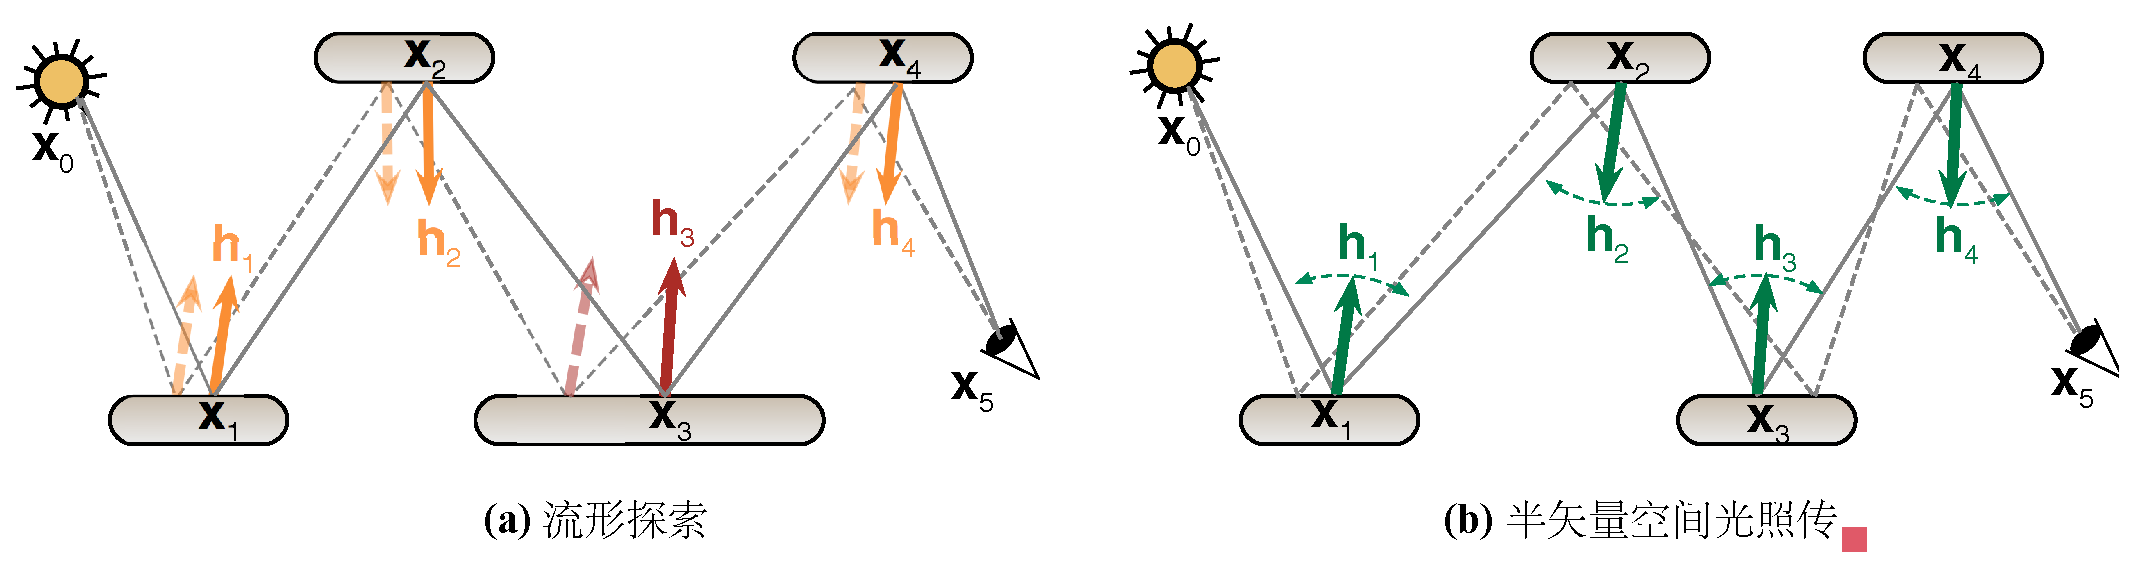
\includegraphics[width=1.0\thewidth]{figures/mlt/me-vs-hslt}
	\caption{在流形探索中,为了处理光泽反射,在每次迭代中它随机地在所有光泽顶点中选取一个顶点当做非镜面顶点(如(a)中的顶点$\mathbf{x}_3$),而保留其他光泽顶点为镜面顶点进行处理;而在半矢量空间光照传输(b)中,首先直接对所有半矢量同时执行一个突变,然后利用牛顿法来逼近满足该突变半矢量的合法路径,并且由于半矢量之间的相关性极小,可以同时按每个顶点的BRDF分布函数进行重要性采样,这是绝大部分路径采样都无法做到的}
	\label{f:mlt-me-vs-hslt}
\end{fullwidth}
\end{figure}

图\ref{f:mlt-me-vs-hslt}(b)中显式了上述半矢量空间路径突变的一个示例。在流形探索中,如图\ref{f:mlt-me-vs-hslt}(a)所示,由于它仅能处理镜面路径,所以它通过随机的识别路径中的一个顶点为非镜面顶点,并保留其他顶点为镜面顶点来处理光泽路径,这样综合下来,路径能够在围绕镜面路径的一个很窄的邻域内进行探索,从而实现光泽路径的处理。然而其中的顶点在镜面与非镜面中的选择非常复杂,并且选择为光泽反射的顶点无法根据其BRDF分布进行重要性采样,路径的贡献值可能很低;与之相反,半矢量空间光照传输可以同时针对所有顶点的BRDF分布执行重要性采样,并且不需要区分顶点为镜面或非镜面顶点。特别地,当某个顶点$\mathbf{x}_i$为镜面顶点时,此时可以设置$\Delta\mathbf{h}^{\perp}_i=\mathbf{0}$,此外不需要做其他特别处理,如果所有顶点都是镜面顶点,则半矢量空间光照传输返回到流形探索(当然这里需要根据后面介绍的方法,将基于半矢量的增量转变基于末端顶点$\mathbf{x}_k$的增量)。



\paragraph{接受率}
半矢量空间的突变路径的接受概率$\min(1,a)$的计算相对比较简单,这里需要注意它们都需要在路径空间进行计算,设当前路径为$\mathbf{X}_t$,通过前面介绍的方法计算的突变路径为$\mathbf{X}_{t+1}$,首先路径的贡献值$f(\mathbf{X}_{t+1})$可以直接通过顶点的表面属性计算而出。对于转移概率$T(\mathbf{X}_t\to\mathbf{X}_{t+1})$,由于我们是在半矢量空间执行转移操作的,因此我们需要首先计算出半矢量的转移概率$T(\mathbf{H}^{\perp}_t\to\mathbf{H}^{\perp}_{t+1})$,然后再变换回路径空间,而前者的值实际上是由每次单个迭代的半矢量转移概率的乘积$p(\mathbf{h}^{\perp}_{t+1}|\mathbf{h}^{\perp}_t)$,因此总的$a$值中的$R$项可以表述为:

\begin{equation}
\begin{aligned}
	R_{t+1}&=f(\mathbf{X}_{t+1})/\Biggm(T(\mathbf{H}^{\perp}_t\to\mathbf{H}^{\perp}_{t+1})\Biggl|\frac{{\rm d}\mathbf{H}^{\perp}}{{\rm d}\mathbf{X}}\Biggl|\Biggm)\\
	&=f(\mathbf{X}_{i+1})\Biggl|\frac{{\rm d}\mathbf{X}}{{\rm d}\mathbf{H}^{\perp}}\Biggl|/T(\mathbf{H}^{\perp}_t\to\mathbf{H}^{\perp}_{t+1})
\end{aligned}
\end{equation}

\noindent 在上式中,分子项可以很容易地通过式\ref{e:mlt-half-vector-space-jacobian}计算而出,因此总的计算比较简单。





\paragraph{半矢量突变的重要性采样}
前面已经讨论了在半矢量空间进行路径突变的思路,但是我们没有说明怎样对半矢量进行突变采样,怎样对顶点的BRDF分布进行重要性采样,以及使用什么样最优化的步幅对半矢量进行突变采样,本节将对这些问题进行介绍。

这涉及两个问题需要解决,首先需要将表面的BRDF分布表述在局部坐标系中,然后对该表述进行直接采样即可。对于第一个问题,首先我们假设所有的BSDF分布都可以表述为贝克曼分布(Beckmann distribution)\myindex{贝克曼分布}{Beckmann distribution}\cite{a:Bidirectionalalightcuts,a:TheScatteringofElectromagneticWavesfromRoughSurfaces,a:AReflectanceModelforComputerGraphics}指出贝克曼分布可以投影到一个平行于并距顶点正切面距离为1的平面,如图\ref{f:mlt-plane-plane}(a)所示,其投影形成一个围绕法线的2D的高斯分布,其方差为$\sigma^{2}=a^{2}/2$,这里$a$为贝克曼分布中的参数,其值$a=\arccos(\mathbf{n}_i\cdot\mathbf{h})$,这种表述称为平面-平面参数化(plane-plane parameterization),其作用域可以使用投影半矢量$\mathbf{h}^{\perp}$表述为:

\begin{equation}\label{e:mlt-parallel-half-vector}
	\mathbf{h}^{||}=\mathbf{h}^{\perp}/\sqrt{1-|\mathbf{h}^{\perp}|^{2}}
\end{equation}

相关数学理论\cite{b:MarkovChains:GibbsFieldsMonteCarloSimulationandQueues}指出在该2D高斯分布上执行马尔可夫链随机行走的最优的接受率为35\%,其对应的最优随机行走步幅为$s=(2/\pi)|\sum|$,这里$\sum$表示BSDF对应2D高斯分布的协方差矩阵。由此可以进一步计算在在平面-平面参数化表述中,单个半矢量的最优化步幅为:

\begin{equation}
	s^{||}_{\max}=a/\sqrt{\pi}
\end{equation}

也就是说,当我们对每个半矢量执行突变时,其突变的步幅(当前半矢量到突变半矢量的距离)的期望值的最大值应该等于该顶点BSDF分布投影到平行平面上形成的2D高斯分布的最优步幅值$s^{||}_{\max}$,这样的步幅选择能够在2D高斯分布上实现最快的探索。

下面我们来介绍怎样将该最优步幅值运用于半矢量突变采样中。

平面-平面和正切面投影是半矢量的两种不同表述方式,但是它们存在很大的区别,正切面投影是一般的垂直投影,投影到一个位于正切面上的单位圆的区域形成投影半矢量$\mathbf{h}^{\perp}$,即$|\mathbf{h}^{\perp}|=\sqrt{h^{2}_x+h^{2}_y} \leq 1$,如图\ref{f:mlt-plane-plane}(b)所示;而平面-平面投影并不是普通的垂直投影,它是直接延长半矢量$\mathbf{h}$直至与平行平面相交,形成平行平面半矢量$\mathbf{h}^{||}$,因此平行半矢量的作用域是整个平面空间,即$\mathbf{h}^{||}\equiv\mathcal{R}^{2}$,如图\ref{f:mlt-plane-plane}(a)所示,你可以想象当半矢量$\mathbf{h}$与法线的夹角接近$90^{\circ}$时,平行半矢量的每个分量标量值将接近无限大,即式\ref{e:mlt-parallel-half-vector}中的分母趋近于0。

\begin{figure}
	\sidecaption
	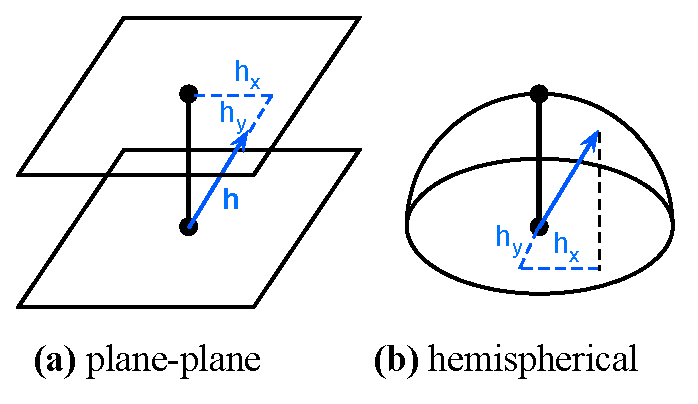
\includegraphics[width=0.65\textwidth]{figures/mlt/plane-plane}
	\caption{(a)为平面-平面参数化,即将半矢量投影到平行于正切面,并距正切面一个单位的平行平面上,形成平行半矢量$\mathbf{h}^{||}$;(b)为半球面参数化,半矢量直接投影到正切面上,形成投影半矢量$\mathbf{h}^{\perp}$}
	\label{f:mlt-plane-plane}
\end{figure}

接下来,我们需要确定使用哪一个参数化的表述对半矢量的微分(或者说半矢量的一阶近似)进行采样,原始的雅可比矩阵$J$(式\ref{e:mlt-hslt-jacobian})显然是要求对投影半矢量空间(即${\rm d}\mathbf{h}^{\perp}$)进行采样的,这也是\cite{a:TheNaturalConstraintRepresentationofthePathSpaceforEfficientLightTransportSimulation}的选择。但是这样的选择会带来一些问题:因为投影半矢量$\mathbf{h}^{\perp}$所在的区域是一个单位圆,而流形上顶点位置的增量$\Delta\mathbf{x}$仅仅是一个一阶近似值,所以它很有可能导致映射的$\Delta\mathbf{h}^{\perp}$超出了这个圆形区域,而这些值会被截断而导致可能合法的路径被直接拒绝,为了防止这个问题,\cite{a:TheNaturalConstraintRepresentationofthePathSpaceforEfficientLightTransportSimulation}将采样值通过压缩变换将其限制在这个单位圆形区域。

前面我们得到了最优的半矢量突变步幅,但我们不能直接对顶点的BSDF分布进行采样来对半矢量进行突变,而是需要以当前半矢量为中心来进行突变,这是一种随机行走而不是随机取样。实践中,\cite{a:TheNaturalConstraintRepresentationofthePathSpaceforEfficientLightTransportSimulation}首先围绕当前半矢量建立一个2D的反射高斯分布(即是相当于固定光的入射方向),并对该分布使用前面提供的最优步幅进行采样,然后将该高斯分布变换到投影半矢量空间。这种方法会导致一些像素扭曲,\cite{a:ImprovedHalfVectorSpaceLightTransport}则直接对平面-平面空间进行采样,其渲染结果得到了改进,例如由于光线微分得到更精确的表述,当半矢量的方向接近正切面时(此时$|\mathbf{h}^{\perp}|$的值接近1)由于避免了可能引起的截断,对突变的接受率更稳定,这里不再对其进行讨论,其主要是涉及一些比较繁琐的变量变换。




\subsubsection{图像平面突变}
上一节讨论的突变方法让路径的两端$\mathbf{x}_0$和$\mathbf{x}_k$保持固定,然后对其他顶点$\mathbf{x}_i$的半矢量(也即是BSDF分布)执行突变,我们称这样的突变方法为BSDF突变。尽管这样的突变方法能够针对光泽顶点的BSDF分布进行重要性采样,它却不能使突变有效地均匀分布于图像平面,本节我们对BSDF突变进行修改使其能够在图像平面均匀突变,因此也称其为图像平面突变。

为了将BSDF突变运用图像平面突变中,考虑如图\ref{f:mlt-image-plane-perturbation}所示的路径,其中$\mathbf{x}_0$位于光源,$\mathbf{x}_k$位于摄像机上。为了使突变能够在图像平面均匀分布,我们首先对像素顶点执行一个像素大小的偏移,并计算对应$\mathbf{x}_{k-1}$顶点的增量$\Delta\mathbf{x}_{k-1}$。

\begin{figure}
	\sidecaption
	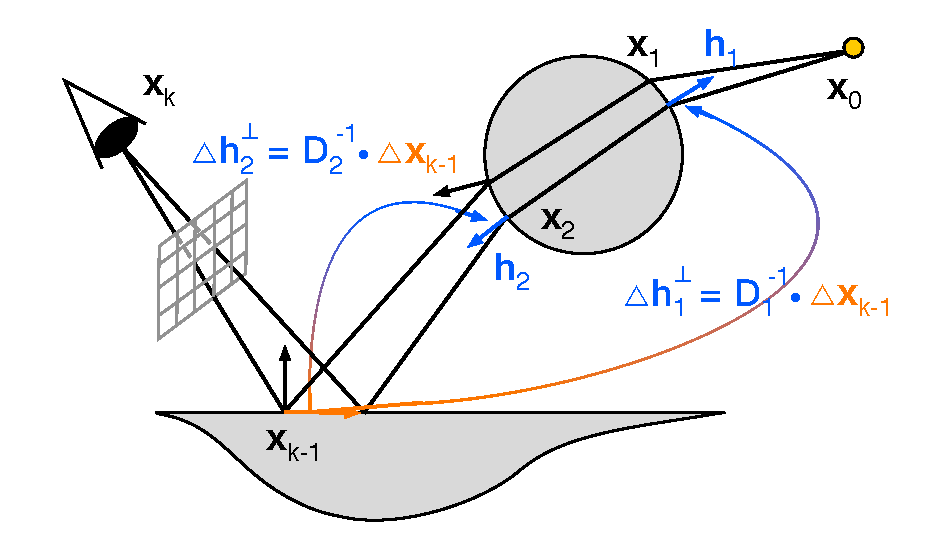
\includegraphics[width=0.65\textwidth]{figures/mlt/hslt-perturbation}
	\caption{在图像平面突变中,首先对像素顶点执行一个像素大小的突变,并计算该摄像机光线在场景中第一个交点的微分$\Delta\mathbf{x}_{k-1}$,然后我们通过变量之间的偏导数将该位置增量转变为各个顶点半矢量的增量,这样最终将图像平面突变转变成了BSDF突变}
	\label{f:mlt-image-plane-perturbation}
\end{figure}

在BSDF突变中,对任意一个顶点执行半矢量突变$\Delta\mathbf{h}^{\perp}_i$之后,我们可以通过雅可比矩阵计算出该半矢量突变对于其他顶点的位置的影响,因为雅可比矩阵记录了每个变量相对于其他变量的偏导数,例如:

\begin{equation}
	\begin{pmatrix}
		B_1 & C_1    &         &         & 0\\
		A_2 & B_2    &  C_2    &         &  \\
		    & \cdots & \cdots  & \cdots  &  \\
		    &        & A_{k-2} & B_{k-2} & C_{k-1}\\
		0   &        &         & A_{k-1} & B_{k-1}
	\end{pmatrix}^{-1}\begin{pmatrix}
		0\\
		\cdot\\
		\Delta\mathbf{h}_i\\
		\cdot\\
		0
	\end{pmatrix}=\begin{pmatrix}
		0\\
		\cdot\\
		\cdot\\
		0\\
		\Delta\mathbf{x}_{k-1}
	\end{pmatrix}
\end{equation}

因此我们通过执行相反的计算过程,即已知$\Delta\mathbf{x}_{k-1}$,可以通过提取针对其他不同顶点的偏导数形成的一个$2\times 2$的矩阵$D_i$来计算其导致的该顶点半矢量的影响$\Delta\mathbf{h}^{\perp}_i=D^{-1}_i\cdot\Delta\mathbf{x}_k-1$。通过这样的方式,我们将图像空间突变转变成了前面介绍的BSDF突变。






\subsubsection{流形之间的跳跃}
为了满足隐函数定理\cite{b:CalculusonManifolds:AModernApproachtoClassicalTheoremsofAdvancedCalculus},路径的半矢量空间表述是基于每个顶点的局部坐标系建立起来的,而表面顶点的局部坐标系通常仅针对该表面有效,所以我们可以以此为边界来界定当前路径一阶近似的范围,这形成类似如图\ref{f:mlt-submanifolds}(b)中阴影部分所示的子流形。对于一些表面边界非常狭窄,并且多个不同物体紧密分布的场景,突变路径很容易落于相邻物体上,此时我们需要小心处理这种不同子流形空间之间的跳跃。

\begin{figure}
	\sidecaption
	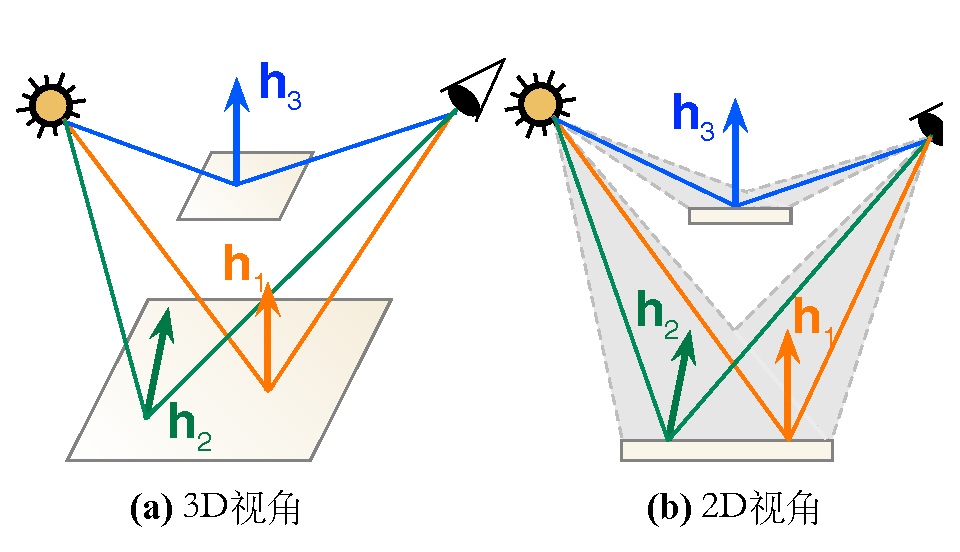
\includegraphics[width=0.65\textwidth]{figures/mlt/submanifolds}
	\caption{路径的半矢量空间表述只是在局部空间(如(b)中的阴影区域)内是合法的,这是由顶点的局部坐标系决定的,所以$\mathbf{h}_1$和$\mathbf{h}_2$是处于同一个子流形,而尽管$\mathbf{h}_1=\mathbf{h}_3$,它们却是处于不同的子流形中}
	\label{f:mlt-submanifolds}
\end{figure}

和流形探索一样,半矢量空间的突变也是需要对突变路径执行反向突变以满足状态之间的连通性,如果突变路径与当前路径处于不同的子流形但是仍然满足其反向突变的,这种路径是可接受的,因为它们是两条合法路径,并且相互之间可以转移;但是需要注意一种特殊情况:即当前路径$\mathbf{X}_i$的建议突变途径$\mathbf{X}_t$处于一个不同的子流形上,其由$\mathbf{X}_t$可以反向转移到“$\mathbf{X}_i$”,但是这个反向转移的路径“$\mathbf{X}_i$”却和原来的路径“$\mathbf{X}_i$”不属于同一子流形,这种情况出现的原因是由于半矢量空间的路径是以半矢量来表述的,但是半矢量是局部的,所以这里虽然半矢量的值是相同的,但是它们分别是针对不同的局部流形区域。针对这种情况,可以记录每个路径顶点所属的表面,然后根据情况进行接受或拒绝。也即是说,流形之间要进行跳跃的条件是相互空间之间能进行转移。

此外,如果路径突变失败(例如由于子流形空间太小等原因),这种情况直接拒绝突变路径会降低路径突变的效率,因为这时流形之间跳跃的情况会比较频繁。对于这种情况,\cite{a:TheNaturalConstraintRepresentationofthePathSpaceforEfficientLightTransportSimulation}会回到原始的MLT算法\cite{a:MetropolisLightTransport}使用的突变方法中:即如果基于当前雅可比矩阵的牛顿迭代法的第一个迭代能够产生一条合法的路径,则接受该路径,但是其转移概率使用传统的基于出射方向突变的方式来计算,这里主要是涉及将各个半矢量的转移概率转换至路径空间。

由此可知,对于BSDF或图像平面突变失败的路径,转移至不同子流形的关键是将基于半矢量空间的突变方法切换回原始的基于出射方向的突变方法,\cite{a:ImprovedHalfVectorSpaceLightTransport}使用了一种更简单的策略,由于它和下面的方法一起组合使用,我们留在下一节讨论。




\subsubsection{综合突变方法 -- 分离策略}
目前讨论的所有突变方法都是对一整条路径执行突变,但这可能在有些情况下并不合适,例如某些部分的满足微分几何的条件很弱(高频率的位移贴图),或者某些部分是完全的漫反射材质,此时迭代速度很慢。\cite{a:ImprovedHalfVectorSpaceLightTransport}借鉴了类似流形探索使用的分段策略,将一条路径分成不同的段,对每个段使用不同的子路径突变来满足不同的需求。

首先,从一条完整路径中选择三个顶点$\mathbf{x}_a$,$\mathbf{x}_b$和$\mathbf{x}_c$,并满足$k\geq a\geq b\geq c\geq 0$,通常选择$a\equiv k$,所以上述的选择将路径划分为三个子路径,这里称其为(注意这里$a,b$和$c$描述的是顶点的位置):

\begin{itemize}
	\item \textbf{多链子路径}$\mathbf{x}_k,\cdots,\mathbf{x}_b$:这部分子路径的目标是实现图像平面的均匀突变,以及在不同子流形之间跳跃,这里使用一种类似传统MLT算法中的多链突变策略(以下会讨论),因此采样是基于出射方向的突变策略,它在$\mathbf{x}_b$处产生一个不同于当前位置的顶点$\mathbf{x}^{'}_b$(因为基于出射方向突变的路径总是无法预测顶点位置),如图\ref{f:mlt-breakup}所示。
	\item \textbf{半矢量空间子路径 }$\mathbf{x}_{b-1},\cdots,\mathbf{x}_{c+1}$:首先连接前一步产生的$\mathbf{x}^{'}_b$点和$\mathbf{x}_{b-1}$点(需要执行可见性判断),形成子路径$\mathbf{x}^{'}_b,\mathbf{h}^{\perp}_{b-1},\cdots,\mathbf{h}^{\perp}_{c+1},\mathbf{x}_c$,如图\ref{f:mlt-breakup}所示,然后固定该子路径的两端,对其执行半矢量空间的突变,参见第\ref{sec:mlt-BSDF-perturbation}节的内容。
	\item \textbf{固定子路径 }$\mathbf{x}_c,\cdots,\mathbf{x}_1,\mathbf{x}_0$:这部分子路径保持不变。
\end{itemize}

\begin{figure}
	\sidecaption
	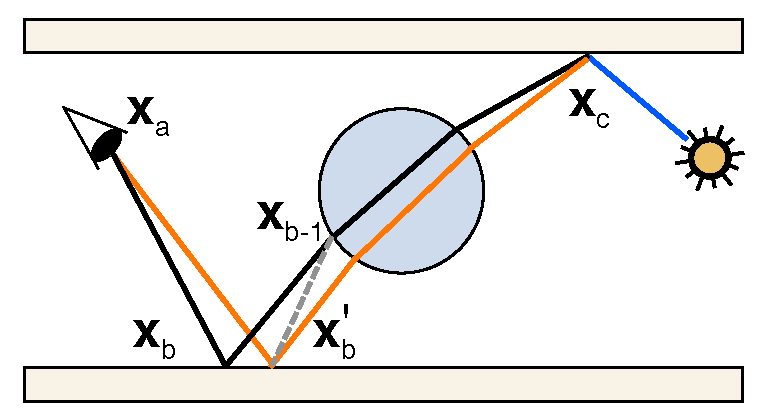
\includegraphics[width=0.55\textwidth]{figures/mlt/breakup}
	\caption{路径被$\mathbf{x}_b$和$\mathbf{c}$分成三段,然后对$\mathbf{x}_k,\cdots,\mathbf{x}_b$执行多链突变,对$\mathbf{x}_{b-1},\cdots,\mathbf{x}_{c+1}$执行半矢量空间的BSDF突变,最后$\mathbf{x}_c,\cdots,\mathbf{x}_1,\mathbf{x}_0$保持不变}
	\label{f:mlt-breakup}
\end{figure}

这里我们将首先介绍多链突变,然后再讨论$b$和$c$点的选择。

多链突变的主要任务是实现图像平面的均匀突变以及子流形之间的转移,它与原始MLT算法中的透镜子路径突变类似。首先它在图像平面上对顶点$\mathbf{x}_a$执行一个像素的偏移,然后执行光线投射查询与场景的第一个交点$\mathbf{x}^{-1}_{k-1}$,此后对顶点的出射方向进行突变采样,然后使用光线投射计算下一个顶点的位置,直到到达$\mathbf{x}^{'}_b$。由于对于出射方向采样来形成路径,因此它不能控制后续顶点的位置。但是它可以很自由地在不同子流形中转移,因为路径空间的突变并没有局部约束的要求。

但与透镜子路径突变不同的是,它的出射方向不是直接对顶点的BSDF分布进行采样而得,而是对顶点的半矢量执行突变,然后将半矢量突变转换到出射方向。这和直接对BSDF采样本没有太多区别,但是其技巧在于它使用了当前路径的顶点和突变路径的顶点的BSDF分布的平均值,这通过将两个BSDF分布函数投影到平面-平面空间的2D高斯分布相加来实现,因为在路径空间两个BSDF函数是没法相加的,这种对平均BSDF分布进行采样使得路径的转移是对称的,简化了接受率的计算,如图\ref{f:mlt-multi-chain-perturbation}所示。

\begin{figure}
	\sidecaption
	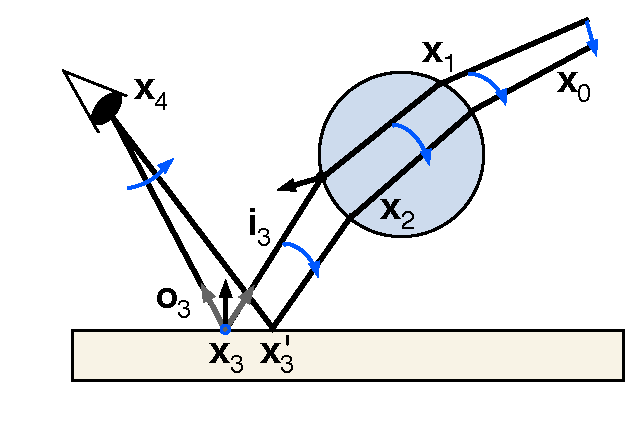
\includegraphics[width=0.55\textwidth]{figures/mlt/multi-chain-perturbation}
	\caption{半矢量空间的多链突变,它首先对像素顶点$\mathbf{x}_4$执行一个像素的偏移,然后使用光线追踪的方式产生后续路径顶点,但是与其不同的是,这里的出射方向是对当前路径和突变路径两个对于顶点的BSDF分布取平均值来采样的,这通过投影到平面-平面空间两个2D高斯分布相加来实现}
	\label{f:mlt-multi-chain-perturbation}
\end{figure}

由于上述的多链突变是不依赖于局部约束的(尽管使用通过对“平均半矢量”进行采样来获得出射方向,但是每个顶点的前后两个相邻顶点并不受这种约束的影响),它本质上是传统的路径采样,所以它并没有子流形限制的问题,可以轻易在子流形之间进行跳跃。这也是多链子路径的重要目标之一。

上述对路径进行分离的策略的效率依赖于$b$和$c$位置的选择。当选择$b=k$时该路径仅包括半矢量空间突变,而选择$b=0$则仅包含多链突变;需要注意对于$b=c$,只有在$b=c=0$的条件下才会发生,因为$\mathbf{x}_b$的位置是会变的,而$\mathbf{x}_c$是固定不变的,所以要想满足这个冲突,只有让$\mathbf{x}_c$落于光源上。

当选择$c=0$时,对路径$\mathbf{x}_0,\cdots,\mathbf{x}_b$执行半矢量突变减少了路径之间的自相关(因为$c$的选择决定两条路径重合的部分的长度,这带来相关性),但是选择较大的$c>0$能够增加计算性能;由于半矢量空间的突变不善于在流形子空间之间进行跳跃,所以选择$b$的一个好的策略是使后面半矢量空间表述的顶点不要落于具有较精细细节的表面。

根据上述分析,\cite{a:ImprovedHalfVectorSpaceLightTransport}使用了一个比较简单的选择策略。首先$b$位于某个顶点$\mathbf{x}_i$的概率正比于该顶点的粗糙度$a_i$,这是因为顶点$\mathbf{x}_b$处要执行连接操作,它需要表面尽可能粗糙:

\begin{equation}
	P(\mathbf{x}_i=\mathbf{x}_b)\sim a_i
\end{equation}

为了能够有几率产生全路径多链突变和全路径半矢量空间突变,相应的分离策略被赋予一个常数:

\begin{equation}
	P(\mathbf{x}_0=\mathbf{x}_b)=P(\mathbf{x}_k=\mathbf{x}_b)\sim 0.1
\end{equation}

最后,为了预防半矢量子路径落于太精细的表面而产生太多子流形之间的跳跃,$c$点的选择被赋予一个同相邻顶点的位置之间的距离因子:

\begin{equation}
	P(\mathbf{x}_i=\mathbf{x}_c)=\sim a_i\cdot||\mathbf{x}_i-\mathbf{x}_{i+1}||^{2}
\end{equation}


%\subsection{流形在直接光源中的运用}
%去掉了MLT的限制
%Manifold Next Event Estimate





 
\section{反向路径采样在MLT算法中的运用}\label{sec:mlt-combine-space}
到目前为止,我们已经学习了两大类MLT算法:一种是基于路径空间的算法,例如传统的MMLT算法,流形探索以及半矢量空间光照传输;另一种是及基于原采样空间的算法,例如PSSMLT算法和MMLT算法。这两种空间的算法都具有不同的优点和缺点,并且几乎其中一类方法的缺点往往都是另一类方法的优点:例如传统MLT算法具有任意修改路径的能力,但是具有较大的方差且很难控制突变步幅;流形探索和半矢量空间光照传输具有能够探索场景局部几何信息的能力,但是却缺乏全局思维;而原采样空间的PSSMLT算法的突变策略更加简洁,并且其目标分布更平坦,具有更低的方差,但是由于缺乏对路径采样的感知却容易导致涟漪效应。

尽管如此,这两种空间的方法却不能形成有效互补,它们之间的唯一联系是通过一个正向映射将原采样空间的变量转换至路径空间,除此之外PSSMLT算法将路径采样完全视为一个黑盒子。MMLT算法在此基础上将路径的采样权重加入到原采样空间,使原采样空间能够在一定程度上对路径采样进行控制,例如通过改变采样技术来避免突变被“卡”在一些局部区域,这些突变路径被卡住的原因是因为使用了概率更低的采样技术。

然而MMLT算法仍然面临一个问题,即当突变路径的采样技术发生变化时,路径更容易发生更大的改变,使得在采样技术之间突变的路径的接受率极低,如图\ref{f:mlt-disruptive-changes}所示,当前路径是一个使用双向路径采样技术得到的路径:其中摄像机子路径为$\mathbf{x}_1\mathbf{x}_2$,光源子路径仅包含一个顶点$\mathbf{x}_3$,然后两条子路径通过$\mathbf{x}_2$和$\mathbf{x}_3$相连接而成,当我们改变采样技术,使得摄像机子路径仅包含一个顶点,而光源子路径包含两个顶点时,尽管原采样空间的坐标并没有发生变化,却由于几何配置导致不能形成一条有效路径。

\begin{figure}
	\sidecaption
	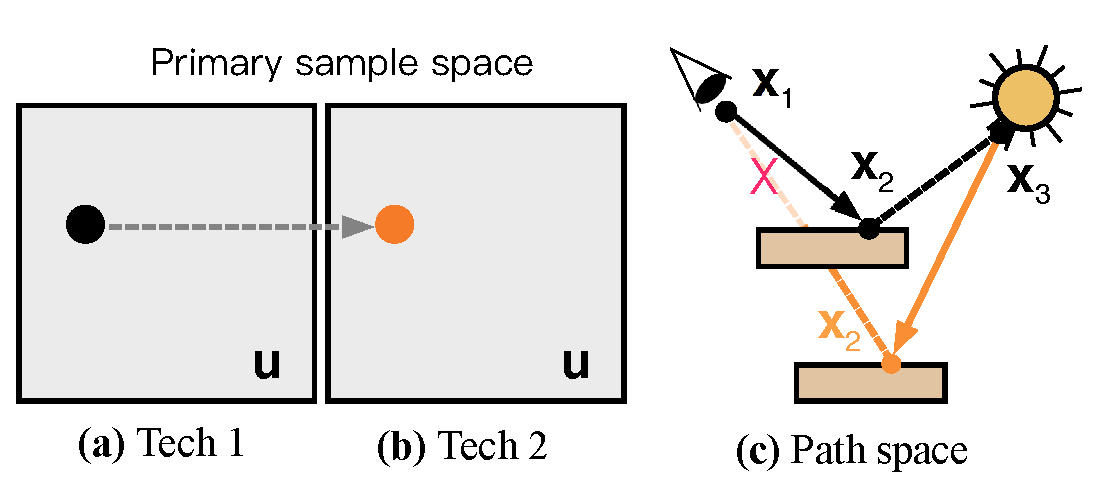
\includegraphics[width=0.65\textwidth]{figures/mlt/disruptive-changes}
	\caption{MMLT算法虽然提供了在采样技术之间进行跳跃的能力,但是采样技术的突变通常导致路径发生较大的改变,使得在采样技术之间突变路径的接受率极低}
	\label{f:mlt-disruptive-changes}
\end{figure}

这种情况出现的原因是由于在原采样空间中采样技术变量$w_t$和路径变量$\mathbf{u}_t$之间是完全独立的,因为原采样空间并不明白一条路径与路径使用的采样技术的相关性,只有路径空间的路径才能计算出路径和采样技术之间的相关性。

为此,我们需要一种机制将路径空间的信息逆向引入至原采样空间,然后指导原采样空间对采样技术进行突变,此时由于路径变量$\mathbf{u}$和采样技术$w$之间不再是完全独立的,因此能够得到接受率更高的采样技术突变。

本节就讨论这种建立原采样和路径空间联系的机制,然后利用它解决两个问题:首先是获得更有效的采样技术突变,以解决上述如图\ref{f:mlt-disruptive-changes}所示的采样技术跳跃问题,其次是能够将两种不同空间的突变策略有效地组合起来。




\subsection{问题分析}
根据序列回火的思想,为了能够对重要性进行采样,MMLT算法将原采样空间扩展成一个离散空间和一个连续空间的乘积,称为复合原采样空间(multiplexed primary space)\myindex{复合原采样空间}{multiplexed primary space},记为:

\begin{equation}
	\mathscr{C}^{k}=\{0,\cdots,k+1\}\times\mathcal{U}^{k}
\end{equation}

\noindent 我们可以将这种表述看成是分解为多个子空间的一个集合$\cup^{k+1}_{i=0}\mathscr{C}^{k}_i$,其中$\mathscr{C}^{k}_i=\{i\}\times [0,1]^{o_k}$,它表示所有长度为$k$的空间中第$i-$个采样技术对应的子空间。

这种子空间划分的目的是为了利用序列回火技术对采样技术进行采样。需要注意的是,这种划分并不是单纯对原采样空间空间位置上的划分,但可以理解为是对扩展空间$\mathscr{C}$的空间划分,这使得每个$\mathscr{C}^{k}_i$都是一个完整的原采样空间,即每个子空间$\mathscr{C}^{k}_i$都包含所有路径。

初学模拟回火或者MMLT算法的时候往往对此是感到迷惑的,这里以MMLT算法为例进行更深入一点分析。首先在模拟回火中,加温的过程是改变分子转移的活跃度,温度参数并不是对状态空间进行分割,相反,不同的温度只是对应不同的转移活跃度,比如更高的温度会使马尔可夫链能够更快地遍历整个状态空间,但是更低的温度下也能遍历整个状态空间,只是会更慢一些。

当然模拟回火已经去掉了温度的原始含义(即高温下所有状态之间的转移效率都更高),而仅仅使用一个能够用来改变状态空间被遍历效率的参数来代替,例如在一个特定的参数下,某些状态之间的转移更高效,而在另一个状态下,另一些状态之间的转移更高效。对于任意一个状态空间,如果我们能够找到一个参数,使得该参数取不同的值时马尔可夫链的遍历具有不同的效率,则该参数可以用来当做模拟回火的温度参数。

回到原采样空间,对于同一长度的所有路径,采样技术正好可以充当这样的“温度”参数:每个路径在不同的采样技术下具有不同的转移效率,并且对于每个采样技术对应的子空间,它能够在只使用该采样技术的情况下遍历整个路径空间,因为每一条路径都能够被该采样技术采样,只是采样效率不一样。

有了上述的描述,就很容易理解一个我们到目前为止可能没有察觉的问题:在复合重要性采样中,每个路径的贡献值是该路径所有采样技术对应的贡献值的加权和,即$f(\mathbf{X})=\sum_i w_i f(\mathbf{X})/p_i(\mathbf{X})$,但是在MMLT算法中,我们每次只对路径使用一个采样技术,即去掉了和的形式,因此必然是一个有偏的估计。然而正是由于MMLT算法中每个采样技术对应的子空间能够映射到所有路径(只是采样效率不一样),因此重复无限多次随机采样之后,估计总能覆盖到每个路径的每一个采样技术,因此能够逼近上面采样技术加权和形式的目标函数。

能够说明每个采样技术所在的子空间能够覆盖整个路径空间的例子也可以从PSSMLT算法中观察得到,PSSMLT算法中的目标函数为$f(\mathbf{X})=f(\mathbf{X})/p_i(\mathbf{X})$,这里唯一的不同是没有了权重系数,但是它仍然是只使用一条路径的其中一个采样技术(这里是根据最大值启发式选择的,参见第\ref{sec:mlt-maximum-heuristic}节),这说明它也能遍历整个路径空间。实际上,如果我们让PSSMLT只选择某个固定的采样技术(而不是按最大值启发式进行选择),PSSMLT中的整个原采样空间正好对应于MMLT算法中该采样技术对应的一个子空间。

上述的分析就为理解接下来要介绍的内容打下了重要的基础,正是由于每个原采样子空间都能够覆盖整个路径空间,那么我们就能够找到每个路径${\mathbf{x}}$在每一个原采样子空间$\mathscr{C}^{k}_i$中的对应该子空间采样技术$i$的变量值$(i,\mathbf{u})$,如果我们像这样保持路径不变而仅对采样技术进行修改,那么这样的采样技术突变将不会导致图\ref{f:mlt-disruptive-changes}中出现的问题,因为它们的路径是保持不变的。

接下来我们需要做的就是找到能够在不同原采样子空间之间突变而保持路径不变的映射方法。




\subsection{反向路径采样}
为了解决MMLT算法中由于采样技术的突变导致路径变化过大而接受率过低的情况,例如图\ref{f:mlt-disruptive-changes}所示,\cite{a:ReversibleJumpMetropolisLightTransportusingInverseMappings}基于\cite{a:ReversiblejumpMarkovchainMonteCarlocomputationandBayesianmodeldetermination}提出的可逆跳跃马尔可夫链蒙特卡洛方法(Reversible Jump MCMC,RJMCMC)\mathindex{可逆跳跃马尔可夫链蒙特卡洛方法}{Reversible Jump MCMC}对MMLT算法进行了修改,它可以用一种确定性的方式在采样技术之间进行跳跃,我们称此方法为可逆跳跃梅特波利斯光照传输(Reversible jump MLT,RJMLT)\myindex{可逆跳跃梅特波利斯光照传输}{Reversible jump MLT}。

我们的目标是推导出一个仅针对采样技术进行变更的突变方法。由于并不知道具体的实现方式,所以我们暂时假定一个采样技术突变策略,它保持原采样空间的位置不变,而仅对采样技术进行突变,就如图\ref{f:mlt-disruptive-changes}(a)和(b)那样。设当前原采样空间的状态位于原采样子空间$\mathscr{C}^{k}_i$中,记为$\hat{\mathbf{u}}=(i,{\mathbf{u}})$,我们对其使用一个仅对采样技术进行修改的突变采样$T(i\to j)$以产生一个位于$\mathscr{C}^{k}_j$中的建议路径$\hat{\mathbf{v}}=(j,{\mathbf{u}})$,并且我们暂时假定采样技术的转移是对称的,即$T(i\to j)=T(j\to i)$。

为了保持样本在两个子空间中的位置不变,我们定义一个确定性的映射$h_{ij}:\mathcal{U}^{k}\to\mathcal{U}^{k}$用来将一个子空间的位置映射到另一个子空间,则上述建议路径的接受概率为:

\begin{equation}
	r(\hat{\mathbf{u}}\to\hat{\mathbf{v}})=\frac{C_j(h_{ij}({\mathbf{u}}))T(j\to i)}{C_i({\mathbf{u}})T(i\to j)}|J[h_{ij}]({\mathbf{u}})|
\end{equation}

\noindent 这里$J[h_{ij}]$为映射$h_{ij}$的雅可比矩阵。为了满足上述假设要求,该映射需满足$h_{ij}({\mathbf{u}})={\mathbf{u}}$,所以该雅可比矩阵为一个单位矩阵。对上式进行展开可得:

\begin{equation}
\begin{aligned}
	r(\hat{\mathbf{u}}\to\hat{\mathbf{v}})&=\frac{C_j({\mathbf{u}})}{C_i({\mathbf{u}})}|\mathds{I}|\\
	&=\frac{w_j({\mathbf{u}})C(P^{-1}_j({\mathbf{u}}))}{w_i({\mathbf{u}})C(P^{-1}_i({\mathbf{u}}))}
\end{aligned}
\end{equation}

\noindent 这里$\mathds{I}$表示单位矩阵,如前所述,$P_i$为路径第$i-$个采样技术对应概率密度函数$p_i$的的累积密度函数。

理想地,由于仅仅是针对采样技术进行突变,我们希望该转移的接受概率仅与复合重要性采样的权重系数有关,然而上式却给出了否定答案:即使所有的随机数并没有发生任何变化,但是由于它们使用了一个不同的映射将其转换到路径空间,并且通常情况下$P^{-1}_j({\mathbf{u}})\neq P^{-1}_i({\mathbf{u}})$,所以上述的建议样本产生的路径有可能发生较大变化,例如图\ref{f:mlt-disruptive-changes}所示,这可能导致较低的接受率。

为了解决上述问题,考虑到每个采样技术对应的原采样子空间都能覆盖全部路径,所以我们希望在切换采样技术的时候保持路径空间的路径值不变,这要求我们在$\mathscr{C}^{k}_j$找到一个新的值${\mathbf{v}}$并使得$P^{-1}_j({\mathbf{u}})=P^{-1}_i({\mathbf{v}})$,然后把这种位置由${\mathbf{u}}$到${\mathbf{v}}$的变化也考虑作为跳跃突变的一部分。

假设所有采样技术$P^{-1}_i$都是平滑并且可逆的,则上述突变则很容易通过映射$h_{ij}({\mathbf{u}})=(P^{-1}_j)^{-1}(P^{-1}_i({\mathbf{u}}))$实现,这里$(P^{-1}_j)^{-1}({\mathbf{x}})$表示一个反向采样技术将一个路径映射为一系列产生该路径的[0,1]随机数。此时该映射的雅可比行列式为:

\begin{equation}
\begin{aligned}
	\big|J[h_{ij}]({\mathbf{u}})\big|&=\big|J[(P^{-1}_j)^{-1}\circ P^{-1}_i]({\mathbf{u}})\big|\\
	&=\big|J[(P^{-1}_j)^{-1}](P^{-1}_i({\mathbf{u}}))\big|\cdot\big|J[P^{-1}_i]({\mathbf{u}})\big|\\
	&=\big|J[P^{-1}_j]({\mathbf{v}})\big|^{-1}\cdot\big|J[P^{-1}_i]({\mathbf{u}})\big|
\end{aligned}
\end{equation}

\noindent 这里第一步是根据链式法则推导出的,而第二步使用了反函数定理(inverse function theorem)\mathindex{反函数定理}{inverse function theorem},即$J_{F^{-1}}(F(p))=[J_F(p)]^{-1}$,上式将两个原采样子空间之间映射的雅可比行列式转换成了两个采样技术雅可比行列式的乘积。

根据前面的内容可知(参见第\ref{sec:mlt-pssmlt}节),由原采样空间向路径空间映射$P^{-1}$的行列式正是该路径使用的采样技术的概率密度函数,即$|J[P^{-1}_i](\mathbf{u})|=p_i(\mathbf{u})^{-1}$,所以上述建议路径的接受概率可转换为:

\begin{equation}\label{e:mlt-rjmlt}
\begin{aligned}
	r(\hat{\mathbf{u}}\to\hat{\mathbf{v}})&=\frac{T(j\to i)C_j({\mathbf{v}})}{T(i\to j)C_i({\mathbf{u}})}\frac{p_j({\mathbf{v}})}{p_i({\mathbf{u}})}\\
	&=\frac{T(j\to i)w_j({\mathbf{v}})f_j({\mathbf{v}})p_j({\mathbf{v}})^{-1}}{T(i\to j)w_i({\mathbf{u}})f_i({\mathbf{u}})p_i({\mathbf{u}})^{-1}}\frac{p_j({\mathbf{v}})}{p_i({\mathbf{u}})}\\
	&=\frac{T(j\to i)w_j({\mathbf{v}})f(P^{-1}_j({\mathbf{v}}))}{T(i\to j)w_i({\mathbf{u}})f(P^{-1}_i({\mathbf{u}}))}\\
	&=\frac{T(j\to i)w_j({\mathbf{v}})}{T(i\to j)w_i({\mathbf{u}})}
\end{aligned}
\end{equation}

\noindent 对于上式最后一步,我们使用了$P^{-1}_i({\mathbf{u}})=P^{-1}_j({\mathbf{v}})$来保持路径不变,从而取消可能的路径变化对采样技术变化的影响。

式\ref{e:mlt-rjmlt}具有一些有趣的属性。首先,采样技术转移的接受率仅与两个采样技术之间的相对MIS权重系数有关,这和我们的期望是一致的,这使得我们可以轻易地对每个路径转移至最优的采样技术;其次,路径贡献函数$f$并没有出现在式\ref{e:mlt-rjmlt}中,这使得采样技术的突变不需要重新执行一次路径追踪的过程;最后,式\ref{e:mlt-rjmlt}中的所有项都可以在对采样技术进行突变之前进行计算,其中采样技术权重系数$w_i$和$w_j$可以根据当前路径直接计算出来,而采样技术之间的转移概率$T$也可以从当前路径计算出来(下面即将讨论)。

上述的特性分析使得我们可以以确定性的方式计算出一个最优的采样技术的转移,而不需要实际执行任何路径样本的采样,并且通过设置$T(i\to j)=w_j({u})$,式\ref{e:mlt-rjmlt}的所有项甚至被全部取消,其采样技术转移的接受率变为1。

然而,式\ref{e:mlt-rjmlt}成立的条件是要求所有采样技术的概率密度函数都是可逆的,这对于大多数路径中的采样都是成立的,例如路径追踪中的每个随机数几乎都是按照逆变换算法中[0,1]均匀分布中得到的。但是对于整个路径的采样,仍然存在一些随机数的采样是不可逆的,例如从多个光源中选取一个光源就涉及不可逆的采样,这里一个选择的光源将映射到连续随机数中的多个值。下面我们就讨论怎样处理这种采样技术不可逆的情况。




\subsubsection{不可逆的采样技术}
式\ref{e:mlt-rjmlt}成立的条件是采样技术的概率密度函数是可逆的,即原采样空间向路径空间的映射是单射函数,这个要求对于路径中每个顶点使用的大部分采样技术都是成立的,但是也存在一些采样方法不满足上述的条件,这些方法可能会将多个连续的原采样空间的随机变量映射为一个相同的路径。由于这里的映射函数不再能够通过累积密度函数$P^{-1}$来表示,本节我们将使用$S$来表述原采样空间到路径空间的映射关系。

本节我们主要讨论以下两种情况:

\begin{itemize}
	\item \textbf{多义区间 }原采样空间中某个连续的区间被映射为同一个路径,但是当路径被反向映射回原采样空间时,我们必须得到一个确定的值$u_i$,如图\ref{f:mlt-intervals}和\ref{f:mlt-non-injective}左边小图所示,这种情况的例子如某个随机变量$u_i$被用于对一个离散的值采样(例如从多个光源中选择一个光源的索引值),这时某个区间$u_i\in[a,b]$被映射到同一条路径;另一种情况是某些维度的随机变量可能用不着,例如对于镜面顶点,它的路径是由反射或折射定理确定的,这时该顶点对应的整个维度的随机数可能完全用不着,这些维度上的所有随机数值都映射到相同的路径。
	\item \textbf{多个采样技术的混合 }这种情况涉及对多个采样技术的选择,例如对简单的漫反射和光泽反射的选择,这里根据一个概率值$a_{\text{diffuse}}$选择漫反射或者光泽反射:
	
	\begin{equation}
		S_{\text{phong}}(\mathbf{u})=\begin{cases}
			S_{\text{diffuse}}(\mathbf{u}_2,\cdots) & \text{ 如果 } u_1<a_{\text{diffuse}}\\
			S_{\text{specular}}(\mathbf{u}_2,\cdots) & \text{  其他 }
		\end{cases}
	\end{equation}
	
	\noindent 这里不同的采样技术的选择将决定后续随机数$(\mathbf{u},\cdots)$的用途,即被用于什么样的采样技术,因此它将导致雅可比矩阵在$u_1=a_{\text{diffuse}}$处变得不连续:
	
	\begin{equation}
		J[S_{\text{phong}}](\mathbf{u})=\begin{cases}
			J[S_{\text{diffuse}}](\mathbf{u}_2,\cdots) & \text{ 如果 } u_1<a_{\text{diffuse}}\\
			J[S_{\text{specular}}](\mathbf{u}_2,\cdots) & \text{  其他 }
		\end{cases}
	\end{equation}
\end{itemize}

上述问题无法使用一种确定性的方法来处理这些映射关系,\cite{a:ReversibleJumpMetropolisLightTransportusingInverseMappings,a:ChartedMetropolisLightTransport}使用一种随机反向行走的方法来解决此问题。这是基于这样的观察,即在构建一个MLT算法的突变策略的时候,它并不需要严格准确的反向映射,对我们而言最重要的是,当对一条路径${\mathbf{x}}=\mathbf{x}_0\mathbf{x}_1\cdots\mathbf{x}_k$使用反向映射得到一个随机数矢量$\mathbf{u}$之后,能够使用正向映射得到原来的路径,即:

\begin{equation}
	{\mathbf{x}}=\text{RandomWalk}(\text{InverseRandomWalk}({\mathbf{x}}),k)
\end{equation}

对于多义区间,上述的条件可以通过如下的随机方法来满足。如图\ref{f:mlt-intervals}表示一个原采样空间随机变量$u_1$和其对应的路径空间的采样值,这里路径空间的值为4个离散的值$N1,N2,N3$和$N4$,其对应的采样概率分别为$a_1,a_2,a_3$和$a_4$,这可能是对4个面积光源的选择,其中的概率分别对应每个光源的面积大小。假设$u_1$为某个未知的值,并被转换到路径空间的值为$N3$,如果对于反向映射,我们能够将$N3$值映射到原采样空间红色选段所示的部分,则经过反向映射后的随机数可以再次被正向映射到$N3$值,这就满足了上述的突变条件。

\begin{figure}
	\sidecaption
	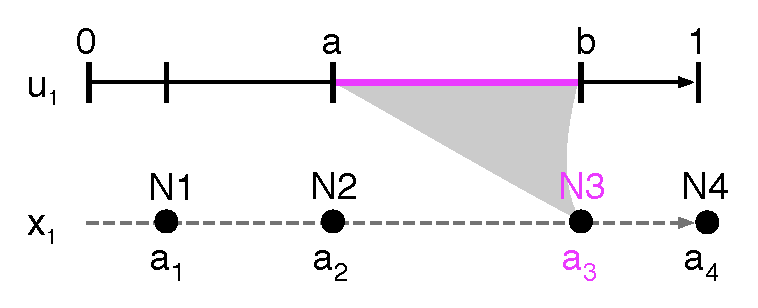
\includegraphics[width=0.55\textwidth]{figures/mlt/intervals}
	\caption{对于多义区间,在不需要知道原始$u_1$值的情况下,只要我们能将$N3$值反向映射到红色线段所示的区间,则该反向映射将满足突变策略要求。这里$a=a_1+a_2$,$b=a+a_3$}
	\label{f:mlt-intervals}
\end{figure}

其中一种方法是直接将$u_1$值传递给路径并保存起来,然后在反向映射的时候直接还原原来的值,但是这给算法带来一定管理的复杂度及存储。根据图\ref{f:mlt-intervals}所示的关系,对于一条路径我们已知的值是$N3$值,以及各个离散变量的概率分布,假设该随机数对应的概率密度为$g$,则可以在反向映射的时候直接使用一个额外的随机数$\upgamma\in[0,1]$来得到一个满足条件的随机的$u_1$值:

\begin{equation}\label{e:mlt-intervals-1}
	u_1=g^{-1}(\upgamma)=a+\upgamma\cdot(b-a)
\end{equation}

\noindent 这样的$u_1$值必然位于$[a,b]$区间,很容易得到对应的雅可比行列式为:

\begin{equation}\label{e:mlt-intervals-2}
	J[g^{-1}](\upgamma)=b-a
\end{equation}

\noindent 为了保证反向映射后的随机数$g^{-1}(\upgamma)$和原始的原采样空间的随机数$u_1$具有相同的分布,我们对$\upgamma$也使用均匀采样,因为原始的$u_1$是均匀采样得到的。

上述的方法称为概率可逆(probabilistic inverse)\myindex{概率可逆}{probabilistic inverse},很容易看出,使用这样的$u_1$值进行正向映射将得到$N3$值。




\paragraph{扩展路径空间}
基于上述的观察和分析,\cite{a:ReversibleJumpMetropolisLightTransportusingInverseMappings}提出一个扩展路径空间(extended path space),它对原始的路径增加了一些辅助维度,用于帮助实现对不可逆采样技术的反向映射。

一条路径只记录各个顶点的信息,它不应该了解任何关于原采样空间的信息,之所以一条“可逆的”路径可以被反向映射到原采样空间,是因为我们知道每个顶点使用的采样技术$p$,例如对应表面的BSDF分布,已知随机数的值(例如出射方向$w_o$的值),并且由于这些采样技术是可逆的,所以我们可以通过反向映射得到每个顶点使用的原采样空间的随机数。但是对于其他一些非顶点采样相关的随机选择,例如选哪个光源,路径并不知道(也不需要)这样的信息,这才使得这样的反向映射变得困难。尽管我们可以让路径额外记住这些状态以帮助反向映射,但是上面的分析使得我们可以仅仅使用一些临时的随机数$\upgamma$就可以实现正确的反向映射。

所以对于反射映射$S^{-1}({\mathbf{x}})$,我们对其参数增加一些额外的维度${\mathbf{\upgamma}}\in[0,1]^{m}$,这些维度对应于那些没有被“记住”的随机数,用于辅助反向映射的过程。所以新的路径扩展空间为$\mathcal{P}\times[0,1]^{m}$,对原采样空间的采样将得到一个扩展路径值$({\mathbf{x}},{\mathbf{\upgamma}})$,然后反向映射函数将作用于这个新的扩展路径,即$S^{-1}({\mathbf{x}},{\mathbf{\upgamma}})$,唯一不同的是,${\mathbf{\upgamma}}$是一个临时的值,它不需要路径保存它,仅在反向映射的时候临时生成,概率可逆的思路保证了反应映射的正确性,如图\ref{f:mlt-non-injective}右边小图所示。

\begin{figure}
	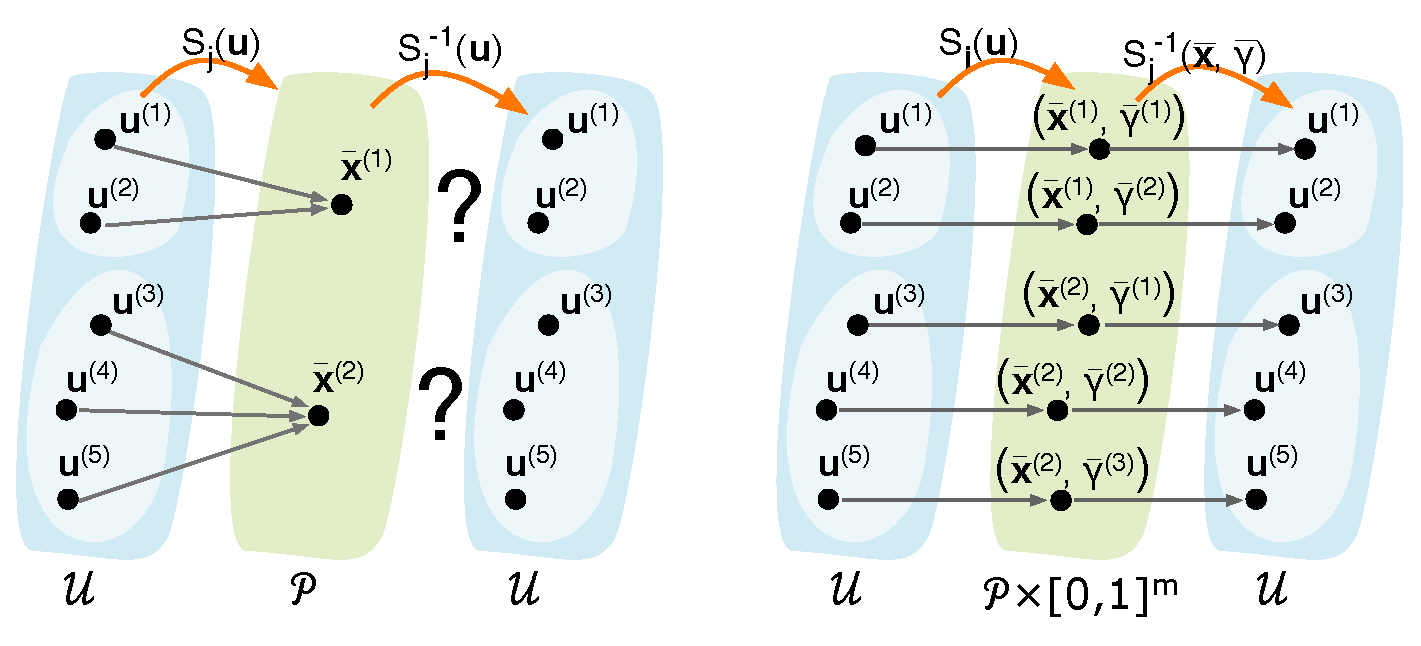
\includegraphics[width=1.\textwidth]{figures/mlt/non-injective}
	\caption{非单射的映射函数$S^{-1}(\mathbf{u})$(左图)破坏了路径由路径空间向原采样空间的反向映射,我们可以通过对路径空间增加一个临时的额外的维度${\upgamma}$来保证反向映射的正确性,这些额外维度的随机数原本也被原采样空间产生,但是我们并不需要记住它们,而代替以一种随机逆向的方法实现这些随机数的双向映射}
	\label{f:mlt-non-injective}
\end{figure}

使用上述的扩展路径空间表述,式\ref{e:mlt-rjmlt}表述的接受率变为:

\begin{equation}\label{e:mlt-rjmlt-general}
\begin{aligned}
	r(\hat{\mathbf{u}}\to\hat{\mathbf{v}})&=\frac{T(j\to i)C_j({\mathbf{v}})}{T(i\to j)C_i({\mathbf{u}})}\frac{\big|J[S_i]({\mathbf{u}})\big|}{\big|J[S_j]({\mathbf{v}})\big|}\\
	&=\frac{T(j\to i)C_j({\mathbf{v}})}{T(i\to j)C_i({\mathbf{u}})}\frac{\big|J[S^{-1}_i]({\mathbf{x}},{\mathbf{\upgamma}})\big|^{-1}}{\big|J[S^{-1}_j]({\mathbf{y}},{\mathbf{\upgamma}})\big|^{-1}}\\
	&=\frac{T(j\to i)C_j({\mathbf{v}})}{T(i\to j)C_i({\mathbf{u}})}\frac{\big|J[S^{-1}_j]({\mathbf{y}},{\mathbf{\upgamma}})\big|}{\big|J[S^{-1}_i]({\mathbf{x}},{\mathbf{\upgamma}})\big|}
\end{aligned}
\end{equation}

\noindent 上式第一步使用了反函数定理。尽管上式看起来很复杂,但是注意这里并不需要记住关于${\upgamma}$的任何状态,它们都是临时重新对$[0,1]$采均匀样产生的。实际上,甚至相关的随机数不需要成为原采样空间需要保存的马尔可夫链状态。

有了上述不依赖于可逆采样的基本框架,让我们再来具体分析相关的一些实例。在路径追踪中,一条路径是按增量的方式从一个顶点开始,然后对每个涉及的采样技术进行随机采样得到的,由于这些采样都是独立的,因此我们可以将路径视为一系列采样的组合:

\begin{equation}
	S_i({\mathbf{u}})=(g_1(\mathbf{u}_1),g_2(\mathbf{x}_1,\mathbf{u}_2),\cdots,g_q(\mathbf{x}_{q-1},\mathbf{u}_q))
\end{equation}

\noindent 这里${\mathbf{x}}_l=\mathbf{x}_1\cdots\mathbf{x}_l$表示到顶点$\mathbf{x}_l$为止的一个子路径,$g_l(\mathbf{x}_{l-1},\mathbf{u}_l)$表示路径上第$l-$个采样技术,注意这里的采样技术是按顶点数量计算的,所以$\mathbf{x}_l$和$\mathbf{u}_l$都表示矢量。对所有采样技术$g_l$执行逆向计算就得到路径的反向映射,则式\ref{e:mlt-rjmlt-general}中的雅可比行列式可表示为每个采样技术反向映射行列式的乘积:

\begin{equation}
	\big|J[S^{-1}_i]({\mathbf{x}},{\upgamma})\big|=\prod^{q}_{l=1}\big|J[g^{-1}_l](\mathbf{x}_l,\upgamma_l)\big|
\end{equation}

\noindent 上式将路径反向映射雅可比行列式的计算转化到对单个采样技术的雅可比行列式的计算,以下我们将对单个采样技术进行分析,并忽略$g_l$中的下标,而直接使用$g$代替每种单个采样技术。

根据目前的分析,采样技术$g$可以分为三种情况。第一种是普通的可逆的采样技术,这包括大部分顶点相关的采样技术,例如顶点的BSDF分布,此时该采样技术的雅可比行列式就是该采样技术的概率密度$p$的倒数,即$|J[S(\mathbf{u})]=p^{-1}$,但需要注意上式中我们需要求的是反向映射的雅可比行列式,所以这里去掉倒数,即$|J[g^{-1}](\mathbf{x},\upgamma)=g|$。

第二种为前面讨论的多义区间的情况,此时原采样空间的某个区间$u\in[a,b]$被映射到路径空间中的一个离散值,对于这种情况,式\ref{e:mlt-intervals-1}和式\ref{e:mlt-intervals-2}提供了该采样技术的反应映射表述,及其雅可比行列式。此外需要注意的是,对于路径中完全没有用到的随机数(例如对于镜面反射,它的出射方向不是对BSDF分布采样得到,而是直接根据反射或折射定理计算而出,这时对应顶点的随机数完全用不到),我们可以认为这里$a=0$,而$b=1$,这变成对整个[0,1]空间的均匀分布,即$g^{-1}(\upgamma)=\upgamma$,其对应的雅可比行列式为1(单位雅可比行列式)。

第三种是多个可选采样技术混合的情况,这种情况略微复杂。假设$g$是一个由$n$个采样技术$g_1,\cdots,g_n$组成的组合,每个采样技术$g_i$被选择的概率为$a_i$。这种情况不同于上面的多义区间,即$u_1$中的每个区间$[a,b]$对应一个特定的离散值;而这里无论选择哪个$g_t$最终都会运用于该点的计算,这有点类似于路径采样技术对原采样空间的划分,每个采样技术对应的原采样子空间都是一个完整的原采样空间,这里无论使用哪个采样技术$g_t$,该采样技术对应的所有区间都能够被顶点采样用到。

而对于一个顶点$\mathbf{x}_i$,它并不会记录该顶点使用了哪一个采样技术$g_t$,它只记录某个被选定的采样技术$g_t$采样产生的一个结果,即出射方向。所以这里相对于多义空间,它“隐藏”了两个随机数,第一个是怎样选择一个采样技术,第二个是将该采样技术对应的值映射到原采样空间随机数$u_1$的哪一区间。也就是说,对于任意一个原采样子空间$\mathbf{u}$,它可以选择任意一个采样技术$g_i$,而同样该顶点在另一个原采样子空间可以选择另一个不同的采样技术$g_j$,它们都能够被映射到同一个顶点$\mathbf{x}$,这就存在着不同原采样子空间之间采样技术$g$之间的转移$T(t)$,我们需要让这种采样技术$g$之间的转移不影响路径的顶点:即让整个两步采样的过程保持均匀,第一步是根据采样技术划分不同的区间,第二步是让对应的采样技术$g$在该区间内均匀分布。

在\cite{a:ReversibleJumpMetropolisLightTransportusingInverseMappings}中使用的雅可比行列式为:

\begin{equation}
	\big|J[g^{-1}({\mathbf{x}},{\upgamma})]\big|=a_t\cdot\big|J[g^{-1}_t]({\mathbf{x}},{\upgamma}_2\cdots)\big|
\end{equation}

\noindent 为了保持整个分布的均匀,其中采样技术$t$的分布服从:

\begin{equation}\label{e:mlt-mixtures}
	T(t)=\frac{a_t\cdot|J[g^{-1}_t]({\mathbf{x}},{\mathbf{\upgamma}})|}{\sum^{n}_{s=1}a_s\cdot|J[g^{-1}_s]({\mathbf{x}},{\mathbf{\upgamma}})|}
\end{equation}

\noindent 当对$t$采样之后,该顶点对应的反向映射及其雅可比行列式为:

\begin{equation}
	|J[g^{-1}]({\mathbf{x}},{\upgamma})|=a_t\cdot|J[g^{-1}_t]({\mathbf{x}},\upgamma_2\cdots)|
\end{equation}




\subsection{RJMLT算法}
经过前面对反向映射的相关讨论,我们能够形成一个确定性的在保持路径不变的情况下在路径的采样技术之间突变的方法,其过程可以描述如下:

\begin{enumerate}
	\item 根据采样技术的重要性分布$w_j(S_i({\mathbf{u}}))$选择一个建议采样技术$j$,实际上我们总是直接选择权重最大的那个采样技术,不涉及采样的过程。
	\item 跳跃到采样技术$j$所在的子空间,并且设置其位置状态为$\hat{\mathbf{v}}=(j,S^{-1}_i({\mathbf{u}}))$。
	\begin{itemize}
		\item 如果路径中存在多义区间,根据式\ref{e:mlt-intervals-1}和式\ref{e:mlt-intervals-2}使用$\upgamma\in[0,1]$上的均匀采样来计算这些随机数的值。
		\item 如果路径中包含多个采样技术的混合,使用式\ref{e:mlt-mixtures}对采样技术进行采样以得到一个采样技术。
	\end{itemize}
	
	\item 最后总是接受$\hat{\mathbf{v}}$。
\end{enumerate}

上述的算法过程不涉及任何对路径的采样,新的样本值完全按确定性的方式计算而出,只有中间一些“隐藏”的随机数需要使用一些临时的均匀分布来随机获取一个值,前面的分析保证这种随机获取的值能够被正确映射。

虽然RJMLT算法能够让路径空间的路径保持不变而在原采样空间对采样技术进行突变,但是这个突变方法也带来一些缺点:它减慢了马尔可夫链在全局探索的速度,因此又不应该频繁使用。\cite{a:ReversibleJumpMetropolisLightTransportusingInverseMappings}将RJMLT算法当做MMLT算法的一种补充,它为原始MMLT算法添加了一种突变方法,新的RJMLT算法包含三种突变,即大步幅突变,原始MMLT算法中的小部分突变(包含原采样子空间内部的突变以及在两个子空间之间的跳跃,但是在跳跃过程中保持位置随机数不变),以及本节介绍的仅在采样技术之间的突变,相应地为它们的使用频率分配10\%,85\%,以及5\%的概率,这些值也可以根据场景及相关测试进行调整。

尽管RJMLT可以处理如多义区间这样不可逆的采样技术,但是它却不能处理那些没有使用逆变换算法的采样技术,例如那些使用取舍算法的采样技术,以及上一章介绍的伍德科克跟踪(Woodcock tracking)\cite{a:TechniquesusedintheGEMcodeforMonteCarloneu-tronicscalculationsinreactorsandothersystemsofcomplexgeometry}。此外,\cite{a:ChartedMetropolisLightTransport}独立地提出了与RJMLT相似的算法,这里不再进行详述。





\subsection{组合原采样空间和路径空间}
由路径空间向原采样空间的反向映射,建立起了一座路径空间和原采样空间两个原本相互独立空间之间的桥梁,它使得我们有机会将两个空间的路径突变技术组合起来,传统单一的正向映射没有这个能力,因为组合两个空间的突变策略需要这样的一个逻辑过程:首先将一个空间中的路径表述转换到另一个空间,并在该空间执行突变,然后将突变结果反向映射回到原路径,以进行接受率计算。它需要一条双向通道,而现在我们已经具备了这样一条双向通道。

由于前面介绍的所有MLT算法的突变策略都可以归结为路径空间(如原始MLT算法,流形探索以及半矢量空间光照传输)或原采样空间(如PSSMLT算法,MMLT算法以及RJMLT算法)的突变策略,现在理论上我们能够将所有这些突变策略组合起来,然后对总的算法随机使用各种突变技术,就能够在总体上结合各种突变策略的优势,例如路径空间的突变策略往往容易更好地探索局部的变化(如流形探索和半矢量光照传输),因为它可以通过仅修改路径中的少量顶点(传统的MMLT算法)或通过局部约束条件来实现突变,然而这种局部特征也使得它很容易被卡在局部,不容易在全局范围内转移;而原采样空间的策略则更容易在全局内实现跳跃,例如RJMLT算法通过在采样技术之间跳跃来实现更“全局”的突变,而与RJMLT算法的思路类似,我们甚至也可以实现不同长度路径之间的跳跃。

有了原采样空间与路径空间之间的相互转换,以及两个空间的各种突变技术,它们之间的组合则非常简单,例如几乎不需要对突变策略做出任何修改,仅仅是路径表述在不同空间之间的转换。我们这里以\cite{a:FusingStateSpacesforMarkovChainMonteCarloRendering}为例对MMLT算法和流形探索算法的组合进行简要介绍。

首先,选择原采样空间为基础空间,即用于记录路径状态以及计算接受率的空间,这里使用的是复合原采样空间,即根据采样技术将原采样空间划分为多个子空间,同MMLT算法一样,这里对每个路径长度使用一条马尔可夫链。

为了兼顾不同突变策略的优点,算法在开始对路径执行突变策略时首先需要随机选择一个突变策略,这里即是在原采样空间和路径空间的突变算法之间选择,这可以是完全随机的,或者根据场景特征或者人工设定某种选择概率分布。不同的空间之间还可以组合多种该空间的突变技术,这对本节讨论的组合算法并没有影响。

如果突变策略方向选择了路径空间,则我们首先需要将当前路径在复合原采样空间的状态表述${\mathbf{u}}$通过前向映射$P^{-1}$转换至路径空间,形成路径空间的表述${\mathbf{x}}$,如图\ref{f:mlt-fusing}左一和左二图,然后在路径空间对当前路径执行某种突变得到路径${y}$,如图\ref{f:mlt-fusing}右二图所示,最后我们在将突变路径${\mathbf{y}}$通过反向映射$P_t$将路径的表述由路径空间转换到原采样空间,形成符合原采样空间的表述${\mathbf{v}}$,如图\ref{f:mlt-fusing}右一图所示。

\begin{figure}
	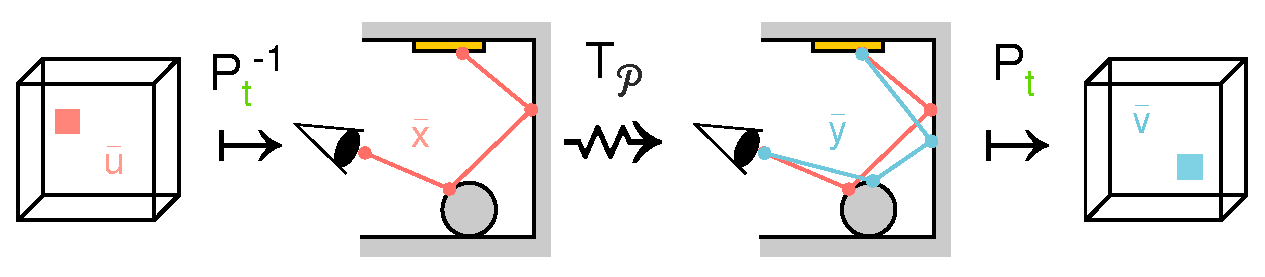
\includegraphics[width=1.0\textwidth]{figures/mlt/fusing}
	\caption{\cite{a:FusingStateSpacesforMarkovChainMonteCarloRendering}中提出的原采样空间和路径空间突变路径的组合策略,以原采样空间作为基础空间,即路径的当前状态记录在原采样空间,当(根据随机选择)需要执行路径空间的突变时,它首先将路径表述由原采样空间通过前向映射$P^{-1}$转换到路径空间,然后在路径空间执行突变,例如可以使用MLT算法或者流形探索等,然后将突变后的路径通过反向映射$P$转换会原采样空间,并计算接受率以决定是否需要接受突变路径}
	\label{f:mlt-fusing}
\end{figure}

最后我们需要在复合原采样空间计算该突变路径的接受概率。由于复合原采样空间的目标分布是一个带权重系数的某个路径单个采样技术的贡献值,所以其接受率的计算需要知道当前路径和突变路径各自使用的采样技术,如式\ref{e:mlt-mmlt-acceptance}所示。然而,与原采样空间的突变策略不一样的是,路径空间的突变技术通常并不依赖于采样技术,因为它们往往是直接对顶点执行修改(如MLT算法),或者对路径按照局部约束执行牛顿逼近计算(如流形探索和半矢量光照传输),因此原采样空间的采样技术对路径的突变并没有用处,并且路径空间突变的路径没法给出一个采样技术的概念。

那么我们怎样选择一个采样技术用于计算接受率呢?这是一个需要小心处理的问题,表面上看,它和前面PSSMLT算法有点类似,即我们需要在多个采样技术之中任意选择一个,但在PSSMLT算法中,由于只有一个原采样空间,所以选择任意采样技术都是可以的,它都可以保证原采样空间的随机数样本能够覆盖整个路径空间。但是在MMLT算法中,原采样空间被按照采样技术划分成多个子空间,每个样本计算的是路径在一个特定采样技术下的贡献值,所以这种采样技术的选择必须满足能够保证所有原采样子空间都能够各自覆盖整个路径空间。

也就是说,对于每个突变路径,它需要有机会在所有原采样子空间之间被计算。一种可能的选择是对路径每个采样技术权重系数的分布进行采样,\cite{a:FusingStateSpacesforMarkovChainMonteCarloRendering}使用一种更简单的策略,即直接保持当前采样技术在整个突变过程中不变,这相当于与采样技术无关,因为路径突变策略本身是能够在整个空间内探索的,所以即是说对于每个采样技术,这种突变都能够保证路径空间的每个路径都可能被覆盖到,这满足复合原采样空间的要求。

这样,通过结合原采样空间和路径空间的突变策略,上述的组合算法能够同时兼顾两种突变策略的优势,形成更健壮的MLT突变策略。





%\section{基于梯度域的方法}\label{sec:mlt-gradient-domain}
%不改变路径采样方法


%\subsection{Improved}
%\subsection{Anisotropic Gaussian Mutations}





\section{组合MC与MCMC算法}\label{sec:mlt-combine}
本章的最后,我们来讨论一下怎样将MCMC算法和MC算法进行组合。

通过到目前为止最近的三章内容,我们已经讨论了离线渲染领域里工业中主流的MCMC算法和MC算法,其中MC算法包括第\ref{chp:path-tracing}章的(双向)路径追踪和第\ref{chp:pm}章的光子映射,这两种方法已经通过第\ref{chp:pm}章介绍的VCM/UPS算法整合到一个框架,而本章目前介绍的都是基于MCMC的方法。这两类方法都有各自的优点,但是没有一种方法能够应付所有不同几何复杂度及光学条件的场景。基于双向路径采样的VCM/UPS算法能够(通过大量重用子路径)高效地处理包含较多光泽面或镜面的场景,但是却不能有效处理包含复杂可见性情况的场景,例如室外的光源通过较小的孔径照亮室内,此种情况下由于MC算法是基于随机采样,样本被均匀分布在整个路径空间,因此那些穿过孔径的少数非常重要的路径样本具有非常低的采样概率,而使收敛速度大大降低;而MCMC算法则非常擅长处理这种具有复杂分布的场景,因为它利用样本之间的相关性(而不是独立地)进行突变采样,如果找到一条重要的路径,则它会连续探索该路径附近局部范围内可能同样非常重要的路径,然而也正是因为这种样本之间的相关性,MCMC算法的最大缺点就是不具备全局思维,例如MCMC算法往往容易被卡在局部区域,其样本也不能有效地均匀分布在图像平面上,其结果是某些局部峰值(即相关性强的)部分呈现非常强的白点,这是因为累积了过多的样本。

\begin{figure}
	\includegraphics[width=1.0\textwidth]{figures/mlt/mlt-correlation}
	\caption{基于流形探索的梅特波利斯光照传输算法(图片来自\cite{a:ManifoldExplorationAMarkovChainMonteCarloTechniqueforRenderingSceneswithDifficultSpecularTransport})}
	\label{f:mlt-mlt-correlation}
\end{figure}

%Metropolis light transport with Manifold exploration (MEMLT) [Jakob and Marschner 2012] suffers from excessive sam- ple correlation in scenes with specular surfaces, which results in its irregular, unpredictable convergence (top row). Despite being based on MCMC sampling, our method (bottom row) shows good convergence properties typical of regular Monte Carlo algorithms: unconverged results provide a reliable preview of the final image, and are amenable to denoising}

因此,我们自然希望能够将MCMC算法和MC算法的优点组合到一起,并且抛弃各自的缺点。然而这看起来是非常困难的,因为它们各自分别使用不同的数学框架,例如MC算法对目标函数使用完全独立的采样,而MCMC算法需要依赖于样本之间的相关性进行采样;MC方法通过计算每条路径的贡献值$f/p$来估计图像的每个像素值,而MCMC算法需要依赖一个已知的像素值的平均值,然后仅通过对样本统计计数来计算每个像素值。

显然我们很难将其统一到一个数学框架中,事实上也最好不要这样做,因为工业中已经有大量的渲染器基于其中之一(或两者)的算法实现,所以我们最好不要对它们各自的基础算法进行较大的变更,而最好能够将两者的结果通过某种简单的形式组合到一起。

以下两点观察有助于探索这样的组合算法:首先,它们都是一个采样算法,它们采样的结果就是一条路径,虽然最终它们对路径的使用方式看起来有点不(实际上)一样,但我们可以仅取各自的路径采样结果即可;其次,在目前几乎所有的离线渲染方案中,路径的采样都涉及顶点的连接,即将两个或多个子路径通过漫反射顶点连接在一起形成一条完整路径,例如传统的双向路径采样是这样,原始MLT中的算法也涉及对部分子路径进行突变,然后与原始路径连接在一起,即使对于流形探索和半矢量光照传输这样的突变策略,它往往也仅仅是对部分子路径使用微分几何进行线性逼近,然后和其他一些子路径进行连接,可见连接对于路径采样是无处不在的。

以上两点观察就给了我们一种启示:将路径分成两段,每段各自分别使用MC算法和MCMC算法,然后将其末端进行连接形成一条完整路径。\cite{a:RobustAdaptivePhotonTracingusingPhotonPathVisibility}首先基于这样的思路将MCMC算法和MC算法进行了融合,但他主要是根据光子映射技术以密度估计的方式进行合并,而借助VCM/UPS框架,\cite{a:RobustLightTransportSimulationviaMetropolisedBidirectionalEstimators}同时将MCMC算法与双向路径追踪和光子映射组合到一起,形成了更健壮的采样方法,这也是本节我们要介绍的方法。





\subsection{平行回火}
虽然最终的全路径是通过MC和MCMC算法的组合连接起来的,但是对于MCMC产生的子路径样本,它的分布的均匀性还是依赖于MCMC算法本身,这会影响到整个图像的估计。我们将看到MCMC部分的子路径实际上用于产生光子图,如果光子图不能有效均匀分布于整个场景,其估计的偏差也会增加。所以我们还是需要在MCMC算法的均匀性上作出一些改进,前面我们已经介绍了序列回火算法来帮助MMLT算法在采样技术之间进行跳跃,然而那仅限于相同长度的路径,本节我们将首先介绍同属于模拟回火的平行回火,它相较于序列回火有更简单的形式,并且能够在不同长度的路径之间进行跳跃。

模拟回火(simulated tempering)\mathindex{模拟回火}{simulated tempering}的目标是将目标函数表述为某个温度参数的形式,这个参数控制着不同状态之间的转移效率,通过在不同参数形式的表述之间进行跳跃,可以有效地防止突变样本被卡在局部区域。这类相关的方法又称为扩展的总体蒙特卡洛方法(Extended Ensemble Monte Carlo)\mathindex{总体蒙特卡洛方法}{Extended Ensemble Monte Carlo}\cite{a:ExtendedEnsembleMonteCarlo}。

根据温度参数的作用不同,目前大概有两类回火算法,第一类即是前面第\ref{sec:mlt-simulated-tempering}节介绍的序列回火(serial tempering)\mathindex{序列回火}{serial tempering},序列回火的温度参数被用于给每个样本在不同的温度下设定一个不同的概率权重$w_i$,以此将目标函数$f(\mathbf{x})$转换为参数化的目标函数$f(\mathbf{x},i)=f(\mathbf{x})w_i$,并使得每个样本在所有温度下的权重和为$\sum_i w_i=1$,这样虽然每个样本在一个特定温度下的估计值$f(\mathbf{x})w_i$是有偏差的,但是通过允许突变在不同温度之间跳跃,这样理论上每个样本有机会遍历每一个温度,所以序列回火对整个和形式$\sum_if(\mathbf{x})w_i$(式\ref{e:mlt-serial-tempering})进行估计,其结果是无偏的。

序列回火是直接作用于原始目标函数$f(\mathbf{x})$的,因此它往往能够通过设计良好的权重控制使突变的全局跳跃更符合目标函数的分布,所以序列回火通常要比我们即将介绍的平行回火工作得更好,甚至某些情况下是平行回火很难处理的\cite{a:AnnealingMarkovChainMonteCarlowithApplicationstoAncestralInference}。然而,设计良好的权重控制系数通常是很难的,在路径采样中,我们正好有针对一条路径样本使用不同采样技术来进行复合重要性采样的历史资产,所以很自然地适用于序列回火算法,这也是MMLT算法的核心思路。但是也正是因为序列回火仅针对原始目标函数进行划分,所以它不适用于路径长度的变化,因为本质上不同的路径长度代表着不同的目标函数,虽然把低维的样本看做是一些维度的值为0进行混合没什么问题,但是由于路径长度的改变往往形成较大的突变,长度的突变加上采样技术的突变会导致序列之间的跳跃被接受的概率更低,所以MMLT算法对每个长度的路径使用一个单独的马尔可夫链。

平行回火(parallel tempering)\mathindex{平行回火}{parallel tempering)}\cite{a:MarkovChainMonteCarloMaximumLikelihood}是一种更简单的用于实现MCMC采样在全局跳跃的回火算法。与序列回火针对原始目标函数的结果分配不同的权重进行参数化不同的是,平行回火参数控制着对目标函数$f(\mathbf{x})$进行不同层级的抽象,形成多个不同的目标函数$f_i(\mathbf{x}_i)$,如图\ref{f:mlt-parallel-tempering}所示,这些目标分布可以认为是不同程度的近似,越接近原始目标函数的目标函数与原始目标函数的形状更加相似,而越抽象的目标函数的频率变化会越小,分布越平坦,极端情况下,甚至可以直接使用一个均匀分布\cite{a:RobustAdaptivePhotonTracingusingPhotonPathVisibility}。

\begin{figure}
\begin{fullwidth}
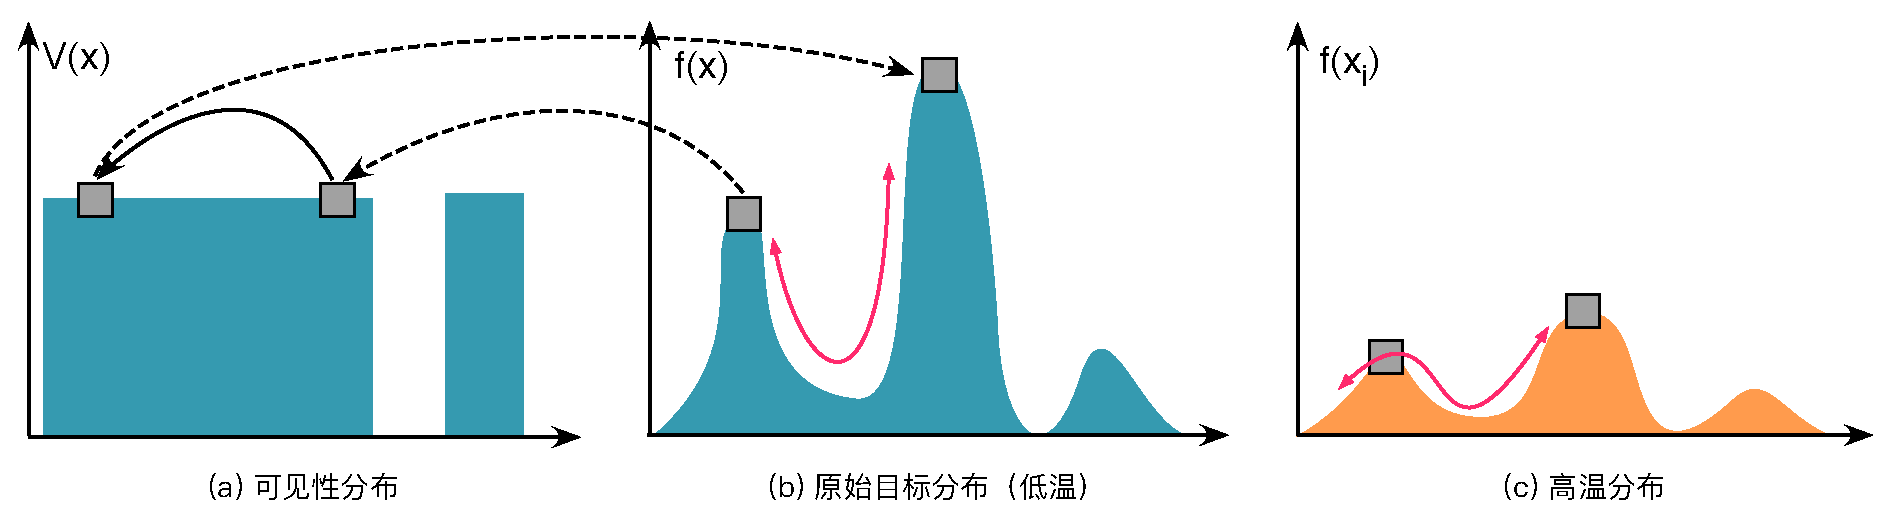
\includegraphics[width=1.\thewidth]{figures/mlt/parallel-tempering}
\caption{平行回火的温度参数将原始目标函数(b)划分成多个不同的目标函数,每个目标函数具有不同的“平坦程度”,更接近原始目标分布的函数能够更好地探索局部,但是往往也容易被卡在局部,例如(b)中凹处,因此太过陡峭,突变的接受率非常低,而导致样本很难摆脱局部区域,但是(c)对应的高温分布则更加平坦,它有利于样本逃离局部区域,极端情况下,如(a)使用的可见性分布,则更加平坦;平行回火通过跳跃到平坦分布进行全局突变,然后回到原始目标分布进行局部突变,以使马尔可夫链的分布更加均匀}
\label{f:mlt-parallel-tempering}
\end{fullwidth}
\end{figure}

平行回火是通过怎样的方式实现马尔可夫链的均匀分布的呢?如图\ref{f:mlt-parallel-tempering}所示,假设中间的函数为原始目标函数,由于其具有两处较大的峰值,因此突变很难由一个峰值转移到另一个峰值,因为这样的突变接受率通常很低,这时候可以使用另一个接近目标分布形状的分布函数来进行采样,如\ref{f:mlt-parallel-tempering}(c)所示,该分布函数由于更加平坦,因此更易于在更大的范围内转移。所以要想实现样本在原始目标函数内均匀地转移,我们可以执行这样的过程:这里以一个更极端的可见性分布(即函数的贡献值大于0则为可见,其值为1,否则为0)为例,如图\ref{f:mlt-parallel-tempering}(a)所示,当原始目标函数的样本被卡在左边的峰值处时,我们可以让其跳转到可见性分布,然后在可见性分布内执行转移,由于可见性分布几乎是(除不可见区域之外)均匀分布,因此更加容易跳转到原始目标函数右边的峰值处,当样本在可见性分布中执行完突变之后,在转移回原始目标分布,这样就完成了在原始目标分布内实现全局转移的目标。

在马尔可夫链蒙特卡洛方法中,我们对一个特定的目标函数使用一个马尔可夫链,因为马尔可夫链需要在该函数对应的所有状态之间转移实现对目标函数的采样。但是上述的平行回火算法包含多个不同的目标函数,这就产生多个马尔可夫链,因此平行回火算法要求多个马尔可夫链同时平行地运行,这也正是其平行(parallel)一词的由来。

那多个平行的马尔可夫链是怎样进行状态转移,并且实现不同马尔可夫链之间的跳跃的呢?这里由于每个马尔可夫链都是相互独立的,所以我们可以将它们看成一个乘积的估计形式,即:

\begin{equation}
	f(\mathbf{x}_1,\cdots,\mathbf{x}_m)=\prod^{m}_{i=1}f_i(\mathbf{x}_i)
\end{equation}

\noindent 这里$\mathbf{x}_i$表示一个矢量,它对应于第$i-$个目标分布的马尔可夫链的状态值。总的平行回火算法是$m$个平行的马尔可夫链分别独立地进行随机行走,我们可以将整个乘积形式看成一个大的马尔可夫链,其每个状态的值为一个矢量$(\mathbf{x}_1,\cdots,\mathbf{x}_m)$。由于每个单独的马尔可夫链是满足细致平衡的,并且它们之间相互独立,所以总的乘积形式的马尔可夫链也是满足细致平衡的。

针对上述的马尔可夫链,我们有两种转移规则,它们都能保证整个大马尔可夫链的细致平衡条件。第一个转移规则是单个目标函数内部的转移,由于它们都是使用梅特波利斯算法进行转移的,所以每个马尔可夫链内部的转移自然是满足细致平衡条件的,因此整个马尔可夫链的转移也满足细致平衡条件。

第二种转移规则是在不同目标分布函数之间的跳跃,通常每次仅随机选择两个目标函数进行跳跃,这通过一种交换(swapping)的操作来实现,即将目标函数$f_i(\mathbf{x}_i)$中的样本值用在目标函数$f_j(\mathbf{x}_j)$中,并同时将目标函数$f_j(\mathbf{x}_j)$中的样本值用在目标函数$f_i(\mathbf{x}_i)$中,在这样的交换转移过程中,必须要确保总的马尔可夫链满足细致平衡条件,这可以通过使用如下的接受率来实现,即:

\begin{equation}
	r(\mathbf{x}_i,\mathbf{x}_j)=\min(a,\frac{f_i(\mathbf{x}_j)f_j(\mathbf{x}_i)}{f_i(\mathbf{x}_i)f_j(\mathbf{x}_j)})
\end{equation}

\noindent 上式的证明可以看成是一个目标分布函数$f_i\cdot f_j$由状态$(\mathbf{x}_i,\mathbf{x}_j)$向状态$(\mathbf{x}_j,\mathbf{x}_i)$的转移,这种转移是对称的,因为它们其实是相同的位置在不同目标分布中的计算,因此一个分布中的某个位置始终被转移至另一个分布中的该位置,反之亦然,所以上述的转移概率仅包含函数值的计算。事实上,平行回火算法中平行的马尔可夫链之间的状态能转移的条件也是它们包含重叠的定义域。由此平行回火算法也称为副本交换(replica exchange)\mathindex{副本交换}{replica exchange}。

最后,平行回火算法怎样使用多个平行的马尔可夫链呢?由于梅特波利斯算法使用的目标函数必须是待求积分的被积函数,这样采样得到的样本分布(马尔可夫链)才是符合该被积函数的分布的,因此梅特波利斯算法可以通过对每个状态的统计计数来对积分进行估计。但是平行回火算法中使用的大多数分布函数却不是正比于原始分布函数的,因此通常我们使用原始目标分布函数作为平行回火中的一个目标函数,通过其他各个更平坦的分布函数来帮助原始目标分布进行全局跳跃,而最后我们仅使用原始目标分布函数的马尔可夫链,而丢弃其他所有平行的马尔可夫链。

上述对平行马尔可夫链的使用方式无疑是很浪费的,但是这是由梅特波利斯算法的特性决定的。不过在本节后面介绍的内容中,由于我们仅仅把梅特波利斯算法当做一个采样器,而其中获得的马尔可夫链中的样本被用于传统的蒙特卡洛方法中,由于蒙特卡洛方法可以使用任意分布对一个函数进行估计,这使得我们可以利用平行回火中的所有马尔可夫链,它们相当于是使用了不同的概率密度函数进行采样,因此其结果可以通过复合重要性采样进行复合。




\subsection{AMCMCVCM/UPS基本算法}
现在我们来简要介绍怎样将MC算法和MCMC算法组合在一起。

基于前面介绍的顶点连接和把MLT算法仅当做一个采样器的两个思路,\cite{a:RobustAdaptivePhotonTracingusingPhotonPathVisibility}提出了一种称为自适应马尔可夫链渐进式光子映射(Adaptive Markov chain Monte Carlo Progressive Photon Mapping,AMCMCPPM)\myindex{自适应马尔可夫链渐进式光子映射}{Adaptive Markov chain Monte Carlo Progressive Photon Mapping,AMCMCPPM}的技术,而\cite{a:RobustLightTransportSimulationviaMetropolisedBidirectionalEstimators}在此基础上将PPM部分替换为VCM/UPS算法,实现了双向路径追踪,光子映射和梅特波利斯光照传输三大基础算法的组合。以下我们将以后者为主,按逻辑理解(而不是算法)的顺序对其各个部分的选择及原理给予简单说明。




\subsubsection{怎样组合成全路径}
蒙特卡洛方法实际上包含两个部分:对某个概率密度函数进行采样以及使用这些样本对积分值进行估计。对于前者,传统的MC算法对一个任意概率密度函数$p(x)$采样,当然其估计的效率取决于该概率密度函数和目标函数$f(x)$的相似性,而MCMC算法则通过一种特别的取舍机制使采样的概率分布正比于目标函数,即$p(x)\approx f(x)$;对于后者,传统的MC方法通过计算所有样本的贡献值的平均值来对积分进行估计,即$\sum_if(x_i)/p(x_i)$,而对于MCMC算法,由于采样的概率密度函数正比于目标函数,每个样本的贡献值$f(x_i)/p(x_i)$近似为一个常数,如果我们知道$p(x)$和$f(x)$的比率,则我们可以通过对样本进行计数的方式来对积分值进行估计,在MLT算法中,我们使用另一个传统MC算法(双向路径采样)来计算这个比率。

所以,使用顶点连接将分别由MC算法和MCMC算法采样得到的子路径组合成一条全路径的关键是舍掉MCMC算法的第二步,即仅使用其采样得到的样本值,然后连接两个子路径组合成一条全路径,最后再按传统的MC算法对积分进行近似计算。因此,在这里MCMC算法变成一个单纯的采样器(第\ref{sec:mlt-mcmc-sampler}节)。

接下来是要选择MC算法和MCMC算法各自用于哪部分子路径的采样。由于MC采样算法是完全随机的,因此样本能够更均匀地分布于定义域内,因此也能够更均匀地分布于图像平面(因为路径通过光线投射的方向增量的生成,即摄像机子路径起点能够均匀分布于图像平面,所以全路径也能够均匀分布于图像平面),而这正是MCMC算法比较欠缺的,所以AMCMCPPM算法使用MC算法对摄像机子路径进行采样,而用MCMC算法对光源子路径采样。

具体地,算法首先使用传统的路径追踪从摄像机出发,生成摄像机子路径。为了能够更高效地和光源子路径进行连接,和光子映射技术一样,这里的摄像机子路径的终点位于漫反射表面上。所有摄像机子路径的顶点信息被保存起来,以进行后续的连接和合并操作。

然后,MCMC算法从光源开始对光源子路径进行采样,生成光源子路径。同样,这些路径的终点落于漫反射表面,以便和摄像机子路径进行连接和合并。在\cite{a:RobustAdaptivePhotonTracingusingPhotonPathVisibility}中,他们使用PPM光子映射技术对顶点进行合并,所以MCMC采样得到的光源子路径相当于光子图,但是这里并不是对每个摄像机子路径收集附近的所有光子进行估计,而是将MCMC产生的每个光子洒向附近的每个摄像机子路径进行概率密度估计;而\cite{a:RobustLightTransportSimulationviaMetropolisedBidirectionalEstimators}同时使用了顶点连接与合并(VCM/UPS),所以每个MCMC样本还会随机选择一个摄像机子路径进行直接连接,以形成双向路径采样技术。





\subsubsection{MCMC采样器}\label{sec:mlt-mcmc-sampler}
光源子路径使用MCMC采样器进行采样,关于MCMC采样器我们需要了解它采样的路径表述空间(例如是原始的欧几里得路径空间,还是原采样空间,或者流形等其他空间),其平行回火使用的多个目标分布函数,以及怎样对多个马尔可夫链的采样结果进行组合。以下我们分别展开描述各个部分的内容。




\paragraph{原采样空间及自适应MCMC突变}
由于原采样空间具有更简单的算法结构,这里直接采用原采样空间作为路径的表述空间,并且路径由原采样空间到路径空间的转换很自然地运用了重要性采样,相对于大多数路径空间的MLT算法得到的样本的方差更小,因为这些方法主要通过直接修改顶点(而不是使用重要性采样)以产生突变路径。

尽管原始PSSMLT算法中的突变策略(例如对围绕当前路径样本的高斯分布采样,参见\ref{sec:mlt-pssmlt}节的内容)非常有效,然而这些样本仍然受困于相关性的影响而使得样本被卡在一些局部区域,这导致一些区域出现如较强的亮点。为了减小样本间的相关性,\cite{a:RobustLightTransportSimulationviaMetropolisedBidirectionalEstimators}使用了一种自适应地调整突变步幅的方法,该方法首次由\cite{a:RobustAdaptivePhotonTracingusingPhotonPathVisibility}引入图形学解决光照传输的问题。

在数学中有一类方法称为自适应马尔可夫链蒙特卡洛方法(adaptive Markov chain Monte Carlo methods)\mathindex{自适应马尔可夫链蒙特卡洛方法}{adaptive Markov chain Monte Carlo methods}\cite{a:AtutorialonadaptiveMCMC},它们可以利用已有样本的数据来动态地调整MCMC算法中样本路径的突变步幅,这里使用的是其中一种简单的变体,称为受控的马尔可夫链蒙特卡洛方法(controlled Markov chain Monte Carlo method)\mathindex{受控的马尔可夫链蒙特卡洛方法}{controlled Markov chain Monte Carlo method}\cite{a:Controlledmcmcforoptimalsampling}。

受控的马尔可夫链蒙特卡洛方法的核心思想是,通过一个可自动适应的参数来调整样本的突变,并使得全部突变样本的平均接受率维持在某个最优的值附近。在\cite{a:RobustLightTransportSimulationviaMetropolisedBidirectionalEstimators}中每个突变样本的值由下式决定:

\begin{equation}
	u_{i+1}=u_i+\begin{cases}
		(2\xi)^{1/\theta_i} & \text{if } \xi<0.5 \\
		-(2\xi-1)^{1/\theta_i} & \text{ 其他}
	\end{cases}
\end{equation}

\noindent 其中,$\xi$是一个[0,1]上的均匀随机数,$\theta_i$就是自适应调整的参数,它在每次突变样本$u_{i+1}$被接受或拒绝之后按下式动态地修改:

\begin{equation}
	\theta_{i+1}=\theta_i+\frac{A_{i+1}-A^{*}}{i}
\end{equation}

\noindent 这里$A^{*}$是一个目标接受率,通常取值为0.234,上式保证MCMC算法的平均接受率维持在该值附近,在相关文献中\cite{a:Weakconvergenceandoptimalscalingofrandomwalkmetropolisalgorithms}该值被视作一个最优的全局接受率。




\paragraph{分布函数}
为了产生光源子路径,我们使用梅特波利斯算法对目标函数进行采样,与单纯的MLT算法类似,这要求我们首先定义光源子路径的贡献函数,以及使用的概率密度目标函数。

由于摄像机子路径已经生成,是一些确定的值,所以可以认为任意一条光源子路径的贡献值就是该光源子路径与某个摄像机子路径进行连接或合并形成的全路径的贡献值。根据VCM/UPS框架,每个光子会与多个顶点进行连接与合并,形成多条全路径,通过使用复合重要性采样将这些路径的贡献值组合以来,则一条光源子路径${\mathbf{x}}_{\text{light}}$的贡献函数可以表述为一个和的形式:

\begin{equation}
	C({\mathbf{x}}_{\text{light}})=\sum_{({\mathbf{x}},t)\in\mathcal{P}({\mathbf{x}}_{\text{light}})}\frac{f({\mathbf{x}})w_t({\mathbf{x}})}{p_t({\mathbf{x}})}
\end{equation}

\noindent 这里${x}$表示一条全路径,$t$表示VCM/UPS框架下对应于概率密度$p_t$的采样技术,$C({\mathbf{x}}_{\text{light}})$表示由于光源子路径${\mathbf{x}}_{\text{light}}$形成的对图像的贡献值,$\mathcal{P}({\mathbf{x}}_{\text{light}})$表示光源子路径所在的路径空间。

上述的光源子路径空间$\mathcal{P}({\mathbf{x}}_{\text{light}})$其实相当于PM算法中光子图中的光子所在的路径空间,为了让光源子路径均匀分布于整个场景中,我们需要使用前面介绍的平行回火算法让马尔可夫链均匀分布于整个场景,为此我们需要选择产生多个平行马尔可夫链的目标函数。\cite{a:RobustAdaptivePhotonTracingusingPhotonPathVisibility}使用了一个可见性分布和一个均匀分布,可见性分布是那些所有贡献值大于0的光源子路径,如图\ref{f:mlt-visibility-contribution}左边小图所示,在这个目标函数分布下,样本在大部分区域非常连续均匀,然而在可见性不连续的部分还是存在非连续的区域,这使得局部的突变很难转移到其他连续区域中,为此另一个完全均匀的分布(即一个传统的MC路径采样)被用于可见性分布函数在不同区域之间的跳跃。在该模型下,光子图能够比较均匀地分布于摄像机可见的区域,然而由于目标函数是可见性函数而不是原始的贡献函数,所以光子图的分布通常不能正确反映光照分布,这只有在全部物体表面都是漫反射表面的情况下才有比较好的近似,对于光泽或镜面表面占多数的情形,上述分布会导致图像在光泽面部分有较多的噪点。

为此,\cite{a:RobustLightTransportSimulationviaMetropolisedBidirectionalEstimators}分别使用了一个原始函数分布和一个可见性分布:

\begin{equation}
\begin{aligned}
	p^{*}_\text{con}(C({\mathbf{x}}_{\text{light}}))&=\text{lum}(C({\mathbf{x}}_{\text{light}}))\\
	p^{*}_\text{vis}(C({\mathbf{x}}_{\text{light}}))&=\begin{cases}
		1 & \text{ if }C({\mathbf{x}}_{\text{light}})>0\\
		0 & \text{ 其他}
	\end{cases}
\end{aligned}
\end{equation}

\noindent 这里$p^{*}$表示标量值,原始贡献值函数分布使得光子能够按实际的光照情况均匀分布于整个场景,而可见性分布用于帮助光源子路径在全局内跳跃,因为可见性分布相对于原始贡献函数在大部分区域更平坦,如图\ref{f:mlt-parallel-tempering}(a)和(b)所示。

\begin{figure}
\sidecaption
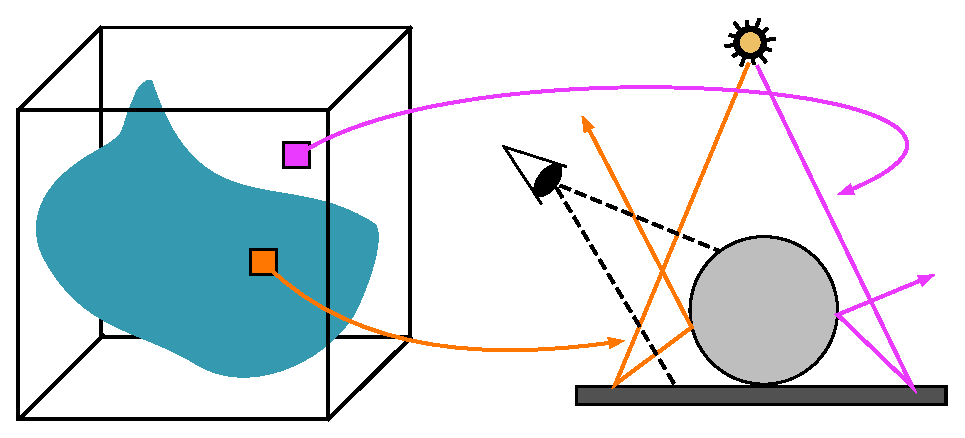
\includegraphics[width=0.6\textwidth]{figures/mlt/visibility-contribution}
\caption{左图为可见性分布函数在原采样空间的样本值,可以看到它非常平坦,存在大片连续区域,有助于原始贡献函数的马尔可夫链在全局区域跳跃}
\label{f:mlt-visibility-contribution}
\end{figure}

为了形成一条全路径,摄像机子路径需要和光源子路径进行连接或合并,对于合并的路径,首先在光源子路径末端的顶点局部范围内进行搜索,以找到所有被该光子影响的摄像机子路径然后按照光子映射技术进行合并;对于连接的路径,每个光源子路径随机选取一条摄像机子路径,然后按照传统的双向路径采样技术一样进行顶点连接形成一条全路径。




\paragraph{规则化系数}
为了使用渐进式光子映射技术,AMCMCVCM/UPS算法需要将总的样本采样划分为多个迭代阶段。和传统的MLT算法一样,我们需要在每次迭代前使用另外一个传统的路径采样方法来计算MCMC算法的归一化常数$b_c={\rm \int}_{\mathcal{U}}p^{c}(C^{*}(u)){\rm d}u$。

然而受限于样本的数量,一般MLT算法中的归一化常数只是一个近似值,而采样平行回火算法的另一个好处是,由于可见性分布几乎接近于一个均匀随机分布,我们可以排除那些不可见的样本,将剩下的样本当做一个均匀分布,这些来自可见性分布函数的样本就类似于来自传统路径追踪采样得到的样本,因此它们可以用于提升归一化常数的精度。所以我们可以在每一次可见性分布函数采用之后重新计算归一化常数:

\begin{equation}
	\langle b_c\rangle=\frac{1}{L}\sum^{L}_{j=1}p^{*}_c(C({x}_{\text{light},j}))
\end{equation}




\paragraph{复合平行马尔可夫链}
传统的平行回火算法通常仅使用与原始目标函数保持相似的目标分布函数对应的马尔可夫链,然而就会浪费大量的其他马尔可夫链的样本值。由于AMCMCVCM/UPS算法将MCMC算法仅当做一个采样器,然后样本值按照传统的MC算法进行估计,这使得我们可以利用平行回火中所有其他目标分布函数的采样结果,因为这仅仅是使用一个不同的概率密度函数进行采样而已,由于每个样本都可以使用这些不同的概率密度函数进行采样,它们的结果可以通过复合重要性采样进行混合:

\begin{equation}
	w_{\text{mcmc}}(x,{x}_{\text{light}})=\frac{\frac{p^{*}_c(C)}{b_c}}{\frac{p^{*}_{\text{vis}}(C)}{b_{\text{vis}}}+\frac{p^{*}_{\text{con}}(C)}{b_{\text{con}}}}
\end{equation}

\noindent 这里$p^{*}_{\text{vis}}$和$p^{*}_{\text{con}}$分别表示可见性分布和原始贡献函数分布的对应的概率密度,而$b_{\text{vis}}$和$b_{\text{con}}$是它们各自的归一化常数。

实际上在PSSMLT算法\cite{a:ASimpleandRobustMutationStrategyfortheMetropolisLightTransportAlgorithm}中使用了类似的思路进行混合,PSSMLT中包含小步幅和大步幅突变,大步幅突变即是一个传统的均匀的路径追踪采样,我们可以将这里的可见性分布函数的采样也看做一个大步幅的突变策略,只需要排除那些不可见的样本,这里的可见性分布和PSSMLT中的大步幅突变就是等效的,实际上在前面计算归一化常数的时候正是排除了不可见的样本,仅保留那些可见的样本用于计算归一化常数。




\subsubsection{VCM/UPS路径复合}
如前所述,AMCMCVCM/UPS是将MCMC算法当做一个光源子路径的采样器,然后将其采样得到的光源子路径与传统的MC算法得到的摄像机子路径通过VCM/UPS空间进行连接或合并形成一条完整的全路径,因此其基础框架仍然是基于VCM/UPS的,因此需要计算每条路径对应每种采样技术的概率密度。这在传统的双向路径追踪算法中是非常简单的,如上一章第\ref{sec:pm-vcm}节的内容所述,然而在PSSMLT框架上,路径的概率密度函数则有点复杂。

在传统的VCM/UPS框架中,我们可以通过对BRDF分布函数等进行重要性采样得到其概率密度函数的值,然而对于PSSMLT算法,原采样空间中具有相同前缀的多个随机数样本都可以产生一条相同的光源子路径,如图\ref{f:mlt-mis-weight}所示,因此即是说一条全路径${x}$可以由无穷多个原采样空间的随机数生成,并且每个随机数都可能具有不同维度(对应不同的路径长度)的目标函数,所以其计算更加复杂。正确的路径概率密度可以表述为:

\begin{equation}
	\hat{p}_t=p_t({x})p_{\mathcal{U},c}({x})=p_t({x}){\rm \int}_{\mathcal{U}_x}\frac{p^{*})c(C^{*}(u))}{b_c}{\rm d}\pi_{{x}}(u)
\end{equation}

\noindent 这里$p_t({x})$是原始双向路径采样技术中对应的采样技术$t$的概率密度函数,它们对于所有能够产生该光源子路径的原采样空间样本$u_0,u_1,\cdots$都是相同的。上式右边的积分可以通过计算这部分重叠的$\mathcal{U}_{{x}}$在原采样空间(一个单位超立方体)中的体积比率来计算。

\begin{figure}
	\sidecaption
	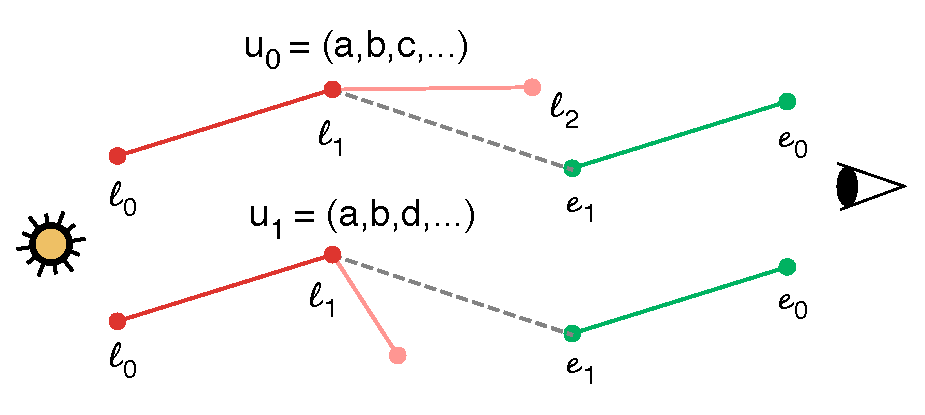
\includegraphics[width=0.65\textwidth]{figures/mlt/mis-weight}
	\caption{通过原采样空间的随机数转换为一条路径,多个具有相同前缀的原采样空间随机数$u_0,u_1,\cdots$会产生一条相同的子路径,因此其路径的概率密度计算变得复杂}
	\label{f:mlt-mis-weight}
\end{figure}

%原始的PSSMLT算法忽略了$p_{\mathcal{U}_c({x})}$而直接使用$p_t({x})$路径的概率密度来近似最终概率密度,即$\hat{p}_t({x})\approx p_t({x})$,虽然这样是不正确的,但是由于计算

\begin{comment}
	

\begin{equation}
	\hat{p}_t({x})=p_t({x}){\rm \int}_{\mathcal{U}_{{x}}}\frac{{\rm d}\pi_{{x}}(u)}{b_{\text{vis}}}\frac{p_t{{x}}}{b\text{vis}}
\end{equation}

\end{comment}


































